\documentclass[twoside]{book}

% Packages required by doxygen
\usepackage{fixltx2e}
\usepackage{calc}
\usepackage{doxygen}
\usepackage[export]{adjustbox} % also loads graphicx
\usepackage{graphicx}
\usepackage[utf8]{inputenc}
\usepackage{makeidx}
\usepackage{multicol}
\usepackage{multirow}
\PassOptionsToPackage{warn}{textcomp}
\usepackage{textcomp}
\usepackage[nointegrals]{wasysym}
\usepackage[table]{xcolor}

% NLS support packages
\usepackage[spanish]{babel}
% Font selection
\usepackage[T1]{fontenc}
\usepackage[scaled=.90]{helvet}
\usepackage{courier}
\usepackage{amssymb}
\usepackage{sectsty}
\renewcommand{\familydefault}{\sfdefault}
\allsectionsfont{%
  \fontseries{bc}\selectfont%
  \color{darkgray}%
}
\renewcommand{\DoxyLabelFont}{%
  \fontseries{bc}\selectfont%
  \color{darkgray}%
}
\newcommand{\+}{\discretionary{\mbox{\scriptsize$\hookleftarrow$}}{}{}}

% Page & text layout
\usepackage{geometry}
\geometry{%
  a4paper,%
  top=2.5cm,%
  bottom=2.5cm,%
  left=2.5cm,%
  right=2.5cm%
}
\tolerance=750
\hfuzz=15pt
\hbadness=750
\setlength{\emergencystretch}{15pt}
\setlength{\parindent}{0cm}
\setlength{\parskip}{3ex plus 2ex minus 2ex}
\makeatletter
\renewcommand{\paragraph}{%
  \@startsection{paragraph}{4}{0ex}{-1.0ex}{1.0ex}{%
    \normalfont\normalsize\bfseries\SS@parafont%
  }%
}
\renewcommand{\subparagraph}{%
  \@startsection{subparagraph}{5}{0ex}{-1.0ex}{1.0ex}{%
    \normalfont\normalsize\bfseries\SS@subparafont%
  }%
}
\makeatother

% Headers & footers
\usepackage{fancyhdr}
\pagestyle{fancyplain}
\fancyhead[LE]{\fancyplain{}{\bfseries\thepage}}
\fancyhead[CE]{\fancyplain{}{}}
\fancyhead[RE]{\fancyplain{}{\bfseries\leftmark}}
\fancyhead[LO]{\fancyplain{}{\bfseries\rightmark}}
\fancyhead[CO]{\fancyplain{}{}}
\fancyhead[RO]{\fancyplain{}{\bfseries\thepage}}
\fancyfoot[LE]{\fancyplain{}{}}
\fancyfoot[CE]{\fancyplain{}{}}
\fancyfoot[RE]{\fancyplain{}{\bfseries\scriptsize Generado por Doxygen }}
\fancyfoot[LO]{\fancyplain{}{\bfseries\scriptsize Generado por Doxygen }}
\fancyfoot[CO]{\fancyplain{}{}}
\fancyfoot[RO]{\fancyplain{}{}}
\renewcommand{\footrulewidth}{0.4pt}
\renewcommand{\chaptermark}[1]{%
  \markboth{#1}{}%
}
\renewcommand{\sectionmark}[1]{%
  \markright{\thesection\ #1}%
}

% Indices & bibliography
\usepackage{natbib}
\usepackage[titles]{tocloft}
\setcounter{tocdepth}{3}
\setcounter{secnumdepth}{5}
\makeindex

% Hyperlinks (required, but should be loaded last)
\usepackage{ifpdf}
\ifpdf
  \usepackage[pdftex,pagebackref=true]{hyperref}
\else
  \usepackage[ps2pdf,pagebackref=true]{hyperref}
\fi
\hypersetup{%
  colorlinks=true,%
  linkcolor=blue,%
  citecolor=blue,%
  unicode%
}

% Custom commands
\newcommand{\clearemptydoublepage}{%
  \newpage{\pagestyle{empty}\cleardoublepage}%
}

\usepackage{caption}
\captionsetup{labelsep=space,justification=centering,font={bf},singlelinecheck=off,skip=4pt,position=top}

%===== C O N T E N T S =====

\begin{document}

% Titlepage & ToC
\hypersetup{pageanchor=false,
             bookmarksnumbered=true,
             pdfencoding=unicode
            }
\pagenumbering{alph}
\begin{titlepage}
\vspace*{7cm}
\begin{center}%
{\Large U\+N\+Virtual\+Lab }\\
\vspace*{1cm}
{\large Generado por Doxygen 1.8.13}\\
\end{center}
\end{titlepage}
\clearemptydoublepage
\pagenumbering{roman}
\tableofcontents
\clearemptydoublepage
\pagenumbering{arabic}
\hypersetup{pageanchor=true}

%--- Begin generated contents ---
\chapter{Indice jerárquico}
\section{Jerarquía de la clase}
Esta lista de herencias esta ordenada aproximadamente por orden alfabético\+:\begin{DoxyCompactList}
\item \contentsline{section}{block}{\pageref{classblock}}{}
\begin{DoxyCompactList}
\item \contentsline{section}{abouttable}{\pageref{classabouttable}}{}
\item \contentsline{section}{adminblock}{\pageref{classadminblock}}{}
\begin{DoxyCompactList}
\item \contentsline{section}{admin2danim}{\pageref{classadmin2danim}}{}
\item \contentsline{section}{admin2deffect}{\pageref{classadmin2deffect}}{}
\item \contentsline{section}{admincontrol}{\pageref{classadmincontrol}}{}
\item \contentsline{section}{adminlogin}{\pageref{classadminlogin}}{}
\item \contentsline{section}{adminlogout}{\pageref{classadminlogout}}{}
\item \contentsline{section}{adminmodel}{\pageref{classadminmodel}}{}
\item \contentsline{section}{adminplot}{\pageref{classadminplot}}{}
\item \contentsline{section}{adminpractice}{\pageref{classadminpractice}}{}
\item \contentsline{section}{adminsection}{\pageref{classadminsection}}{}
\item \contentsline{section}{session\+Manager}{\pageref{classsessionManager}}{}
\end{DoxyCompactList}
\item \contentsline{section}{adminmodelfiles}{\pageref{classadminmodelfiles}}{}
\item \contentsline{section}{anim2d}{\pageref{classanim2d}}{}
\item \contentsline{section}{controls}{\pageref{classcontrols}}{}
\item \contentsline{section}{credits}{\pageref{classcredits}}{}
\item \contentsline{section}{databasemanager}{\pageref{classdatabasemanager}}{}
\item \contentsline{section}{documentation}{\pageref{classdocumentation}}{}
\item \contentsline{section}{erase}{\pageref{classerase}}{}
\item \contentsline{section}{launch}{\pageref{classlaunch}}{}
\item \contentsline{section}{logo}{\pageref{classlogo}}{}
\item \contentsline{section}{menu}{\pageref{classmenu}}{}
\item \contentsline{section}{menuadmin}{\pageref{classmenuadmin}}{}
\item \contentsline{section}{My\+Xml}{\pageref{classMyXml}}{}
\begin{DoxyCompactList}
\item \contentsline{section}{animation2d\+S\+VG}{\pageref{classanimation2dSVG}}{}
\end{DoxyCompactList}
\item \contentsline{section}{outputs}{\pageref{classoutputs}}{}
\item \contentsline{section}{plots}{\pageref{classplots}}{}
\item \contentsline{section}{simulator}{\pageref{classsimulator}}{}
\item \contentsline{section}{S\+V\+Gplot}{\pageref{classSVGplot}}{}
\item \contentsline{section}{tables}{\pageref{classtables}}{}
\item \contentsline{section}{title}{\pageref{classtitle}}{}
\end{DoxyCompactList}
\item \contentsline{section}{configuration}{\pageref{classconfiguration}}{}
\item \contentsline{section}{csvreader}{\pageref{classcsvreader}}{}
\item \contentsline{section}{export}{\pageref{classexport}}{}
\item \contentsline{section}{import}{\pageref{classimport}}{}
\item \contentsline{section}{tlistemysql}{\pageref{classtlistemysql}}{}
\item \contentsline{section}{X\+M\+L\+Thing}{\pageref{classXMLThing}}{}
\end{DoxyCompactList}

\chapter{Índice de clases}
\section{\-Lista de clases}
\-Lista de las clases, estructuras, uniones e interfaces con una breve descripción\-:\begin{DoxyCompactList}
\item\contentsline{section}{\hyperlink{classabouttable}{abouttable} }{\pageref{classabouttable}}{}
\item\contentsline{section}{\hyperlink{classadmin2danim}{admin2danim} }{\pageref{classadmin2danim}}{}
\item\contentsline{section}{\hyperlink{classadmin2deffect}{admin2deffect} }{\pageref{classadmin2deffect}}{}
\item\contentsline{section}{\hyperlink{classadminblock}{adminblock} }{\pageref{classadminblock}}{}
\item\contentsline{section}{\hyperlink{classadmincontrol}{admincontrol} }{\pageref{classadmincontrol}}{}
\item\contentsline{section}{\hyperlink{classadminlogin}{adminlogin} }{\pageref{classadminlogin}}{}
\item\contentsline{section}{\hyperlink{classadminlogout}{adminlogout} }{\pageref{classadminlogout}}{}
\item\contentsline{section}{\hyperlink{classadminmodel}{adminmodel} }{\pageref{classadminmodel}}{}
\item\contentsline{section}{\hyperlink{classadminmodelfiles}{adminmodelfiles} }{\pageref{classadminmodelfiles}}{}
\item\contentsline{section}{\hyperlink{classadminplot}{adminplot} }{\pageref{classadminplot}}{}
\item\contentsline{section}{\hyperlink{classadminpractice}{adminpractice} }{\pageref{classadminpractice}}{}
\item\contentsline{section}{\hyperlink{classadminsection}{adminsection} }{\pageref{classadminsection}}{}
\item\contentsline{section}{\hyperlink{classanim2d}{anim2d} }{\pageref{classanim2d}}{}
\item\contentsline{section}{\hyperlink{classanimation2dSVG}{animation2d\-S\-V\-G} }{\pageref{classanimation2dSVG}}{}
\item\contentsline{section}{\hyperlink{classblock}{block} }{\pageref{classblock}}{}
\item\contentsline{section}{\hyperlink{classconfiguration}{configuration} }{\pageref{classconfiguration}}{}
\item\contentsline{section}{\hyperlink{classcontrols}{controls} }{\pageref{classcontrols}}{}
\item\contentsline{section}{\hyperlink{classcredits}{credits} }{\pageref{classcredits}}{}
\item\contentsline{section}{\hyperlink{classcsvreader}{csvreader} }{\pageref{classcsvreader}}{}
\item\contentsline{section}{\hyperlink{classdatabasemanager}{databasemanager} }{\pageref{classdatabasemanager}}{}
\item\contentsline{section}{\hyperlink{classdocumentation}{documentation} }{\pageref{classdocumentation}}{}
\item\contentsline{section}{\hyperlink{classerase}{erase} }{\pageref{classerase}}{}
\item\contentsline{section}{\hyperlink{classexport}{export} }{\pageref{classexport}}{}
\item\contentsline{section}{\hyperlink{classimport}{import} }{\pageref{classimport}}{}
\item\contentsline{section}{\hyperlink{classlogo}{logo} }{\pageref{classlogo}}{}
\item\contentsline{section}{\hyperlink{classmenu}{menu} }{\pageref{classmenu}}{}
\item\contentsline{section}{\hyperlink{classmenuadmin}{menuadmin} }{\pageref{classmenuadmin}}{}
\item\contentsline{section}{\hyperlink{classMyXml}{\-My\-Xml} }{\pageref{classMyXml}}{}
\item\contentsline{section}{\hyperlink{classoutputs}{outputs} }{\pageref{classoutputs}}{}
\item\contentsline{section}{\hyperlink{classplots}{plots} }{\pageref{classplots}}{}
\item\contentsline{section}{\hyperlink{classsessionManager}{session\-Manager} }{\pageref{classsessionManager}}{}
\item\contentsline{section}{\hyperlink{classsimulator}{simulator} }{\pageref{classsimulator}}{}
\item\contentsline{section}{\hyperlink{classSVGplot}{\-S\-V\-Gplot} }{\pageref{classSVGplot}}{}
\item\contentsline{section}{\hyperlink{classtables}{tables} }{\pageref{classtables}}{}
\item\contentsline{section}{\hyperlink{classtitle}{title} }{\pageref{classtitle}}{}
\item\contentsline{section}{\hyperlink{classtlistemysql}{tlistemysql} }{\pageref{classtlistemysql}}{}
\item\contentsline{section}{\hyperlink{classXMLThing}{\-X\-M\-L\-Thing} }{\pageref{classXMLThing}}{}
\end{DoxyCompactList}

\chapter{Documentación de las clases}
\hypertarget{classabouttable}{}\section{Referencia de la Clase abouttable}
\label{classabouttable}\index{abouttable@{abouttable}}
Diagrama de herencias de abouttable\begin{figure}[H]
\begin{center}
\leavevmode
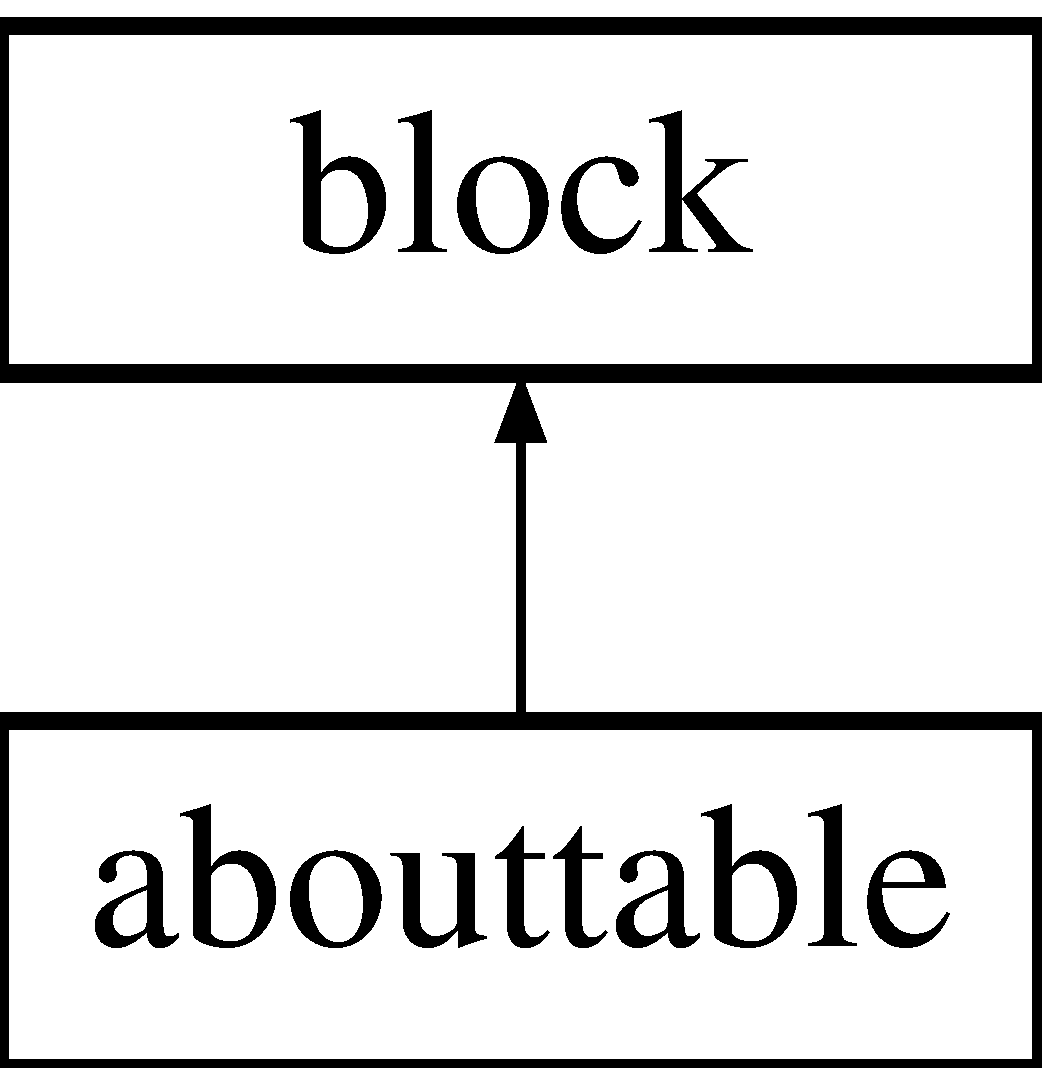
\includegraphics[height=2.000000cm]{classabouttable}
\end{center}
\end{figure}
\subsection*{Métodos públicos}
\begin{DoxyCompactItemize}
\item 
\mbox{\Hypertarget{classabouttable_ac0f2c0d925796601544d584613e05e47}\label{classabouttable_ac0f2c0d925796601544d584613e05e47}} 
{\bfseries display} ()
\item 
\mbox{\Hypertarget{classabouttable_a97836320a206e585f3e682fa570a55b3}\label{classabouttable_a97836320a206e585f3e682fa570a55b3}} 
{\bfseries display\+Model} ()
\item 
\mbox{\Hypertarget{classabouttable_a175c3aa085ab45e2783ee0f5e7929c30}\label{classabouttable_a175c3aa085ab45e2783ee0f5e7929c30}} 
{\bfseries display\+Modellers} ()
\item 
\mbox{\Hypertarget{classabouttable_aea286997a07d462392d4124cb11c38fe}\label{classabouttable_aea286997a07d462392d4124cb11c38fe}} 
{\bfseries display\+Files} ()
\item 
\mbox{\Hypertarget{classabouttable_a53647b9d4cec21fea7c3c5a591561d17}\label{classabouttable_a53647b9d4cec21fea7c3c5a591561d17}} 
{\bfseries display\+Embed\+Links} ()
\item 
\mbox{\Hypertarget{classabouttable_a783812e4a907615c4d195905f695e170}\label{classabouttable_a783812e4a907615c4d195905f695e170}} 
{\bfseries display\+Practices} ()
\end{DoxyCompactItemize}
\subsection*{Otros miembros heredados}


\subsection{Descripción detallada}


Definición en la línea 4 del archivo about.\+php.



La documentación para esta clase fue generada a partir del siguiente fichero\+:\begin{DoxyCompactItemize}
\item 
/home/ogduartev/public\+\_\+html/unvl-\/\+Git\+Hub/\+U\+N\+Virtual\+Lab/about.\+php\end{DoxyCompactItemize}

\hypertarget{classadmin2danim}{}\section{Referencia de la Clase admin2danim}
\label{classadmin2danim}\index{admin2danim@{admin2danim}}
Diagrama de herencias de admin2danim\begin{figure}[H]
\begin{center}
\leavevmode
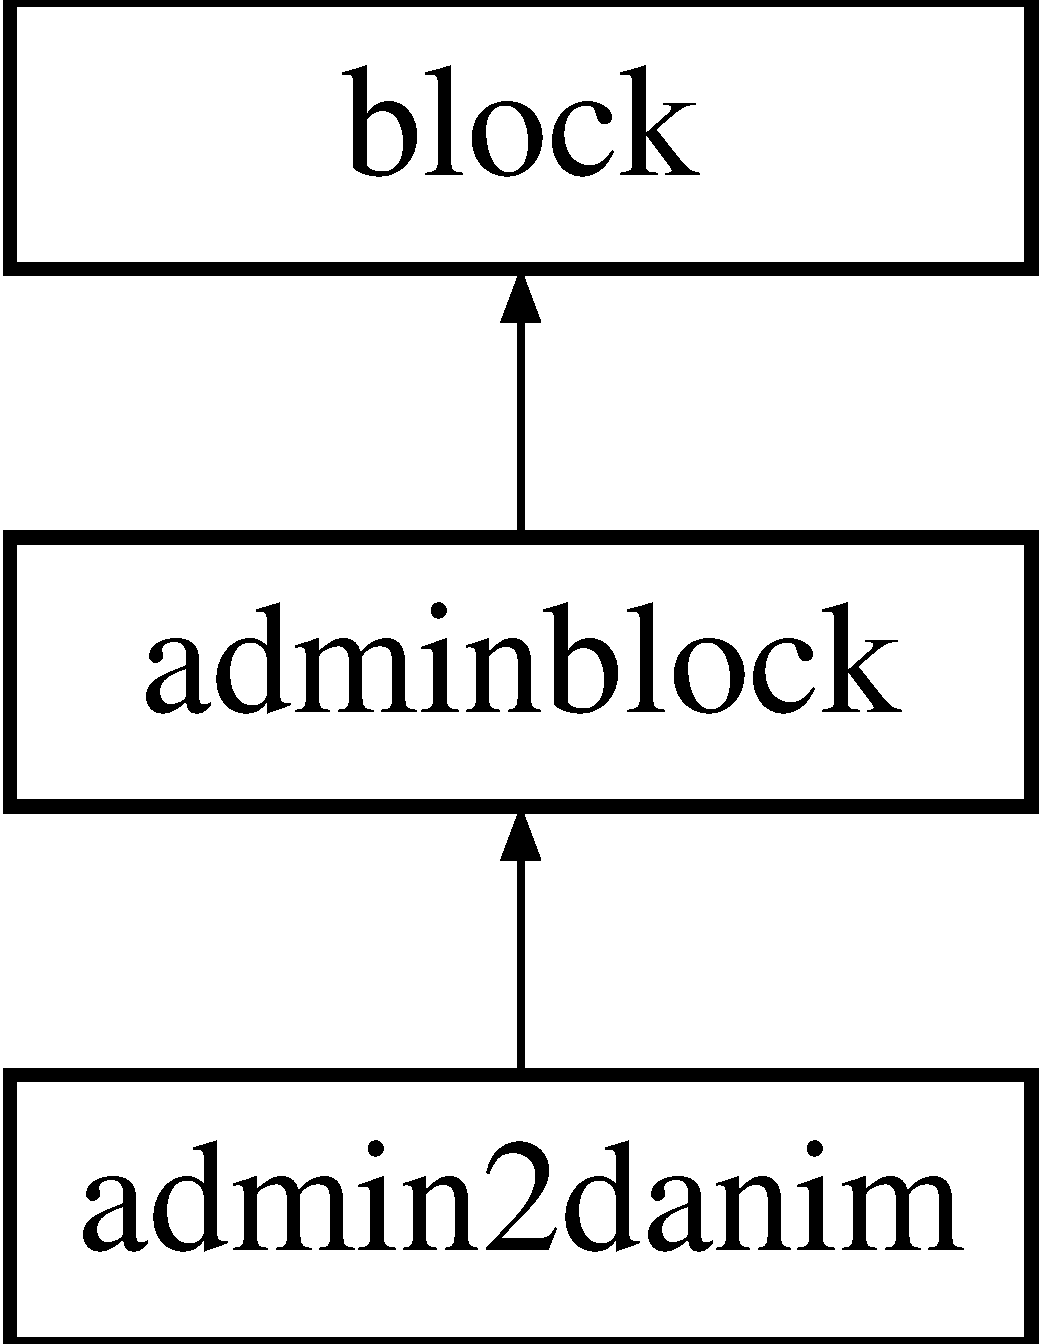
\includegraphics[height=3.000000cm]{classadmin2danim}
\end{center}
\end{figure}
\subsection*{Métodos públicos}
\begin{DoxyCompactItemize}
\item 
\mbox{\Hypertarget{classadmin2danim_a236816c06411884f994a70c97c8f3a71}\label{classadmin2danim_a236816c06411884f994a70c97c8f3a71}} 
{\bfseries create\+Fields} ()
\item 
\mbox{\Hypertarget{classadmin2danim_a3abf1a2202ba64cd5148c8ce93aa60b3}\label{classadmin2danim_a3abf1a2202ba64cd5148c8ce93aa60b3}} 
{\bfseries create\+Relations1N} ()
\item 
\mbox{\Hypertarget{classadmin2danim_aed4665b024fe1b09404d2ad47444f4cf}\label{classadmin2danim_aed4665b024fe1b09404d2ad47444f4cf}} 
{\bfseries create\+Relations1\+N1N} ()
\item 
\mbox{\Hypertarget{classadmin2danim_af8b70fda0c451907be1ddabaf757cd92}\label{classadmin2danim_af8b70fda0c451907be1ddabaf757cd92}} 
{\bfseries find\+Model\+Id} ()
\item 
\mbox{\Hypertarget{classadmin2danim_a047496fc7a4c63d403f2a9aeba9bb0cc}\label{classadmin2danim_a047496fc7a4c63d403f2a9aeba9bb0cc}} 
{\bfseries upload} ()
\item 
\mbox{\Hypertarget{classadmin2danim_a950abe5065035087fa8e9c7478a90482}\label{classadmin2danim_a950abe5065035087fa8e9c7478a90482}} 
{\bfseries display\+Post\+Own} ()
\item 
\mbox{\Hypertarget{classadmin2danim_a04b458e682b3a76d062bc3b686fe4a08}\label{classadmin2danim_a04b458e682b3a76d062bc3b686fe4a08}} 
{\bfseries display\+Anim} ()
\end{DoxyCompactItemize}
\subsection*{Otros miembros heredados}


\subsection{Descripción detallada}


Definición en la línea 5 del archivo admin2danim.\+php.



La documentación para esta clase fue generada a partir del siguiente fichero\+:\begin{DoxyCompactItemize}
\item 
/home/ogduartev/public\+\_\+html/unvl-\/\+Git\+Hub/\+U\+N\+Virtual\+Lab/admin/admin2danim.\+php\end{DoxyCompactItemize}

\hypertarget{classadmin2deffect}{\section{\-Referencia de la \-Clase admin2deffect}
\label{classadmin2deffect}\index{admin2deffect@{admin2deffect}}
}
\-Diagrama de herencias de admin2deffect\begin{figure}[H]
\begin{center}
\leavevmode
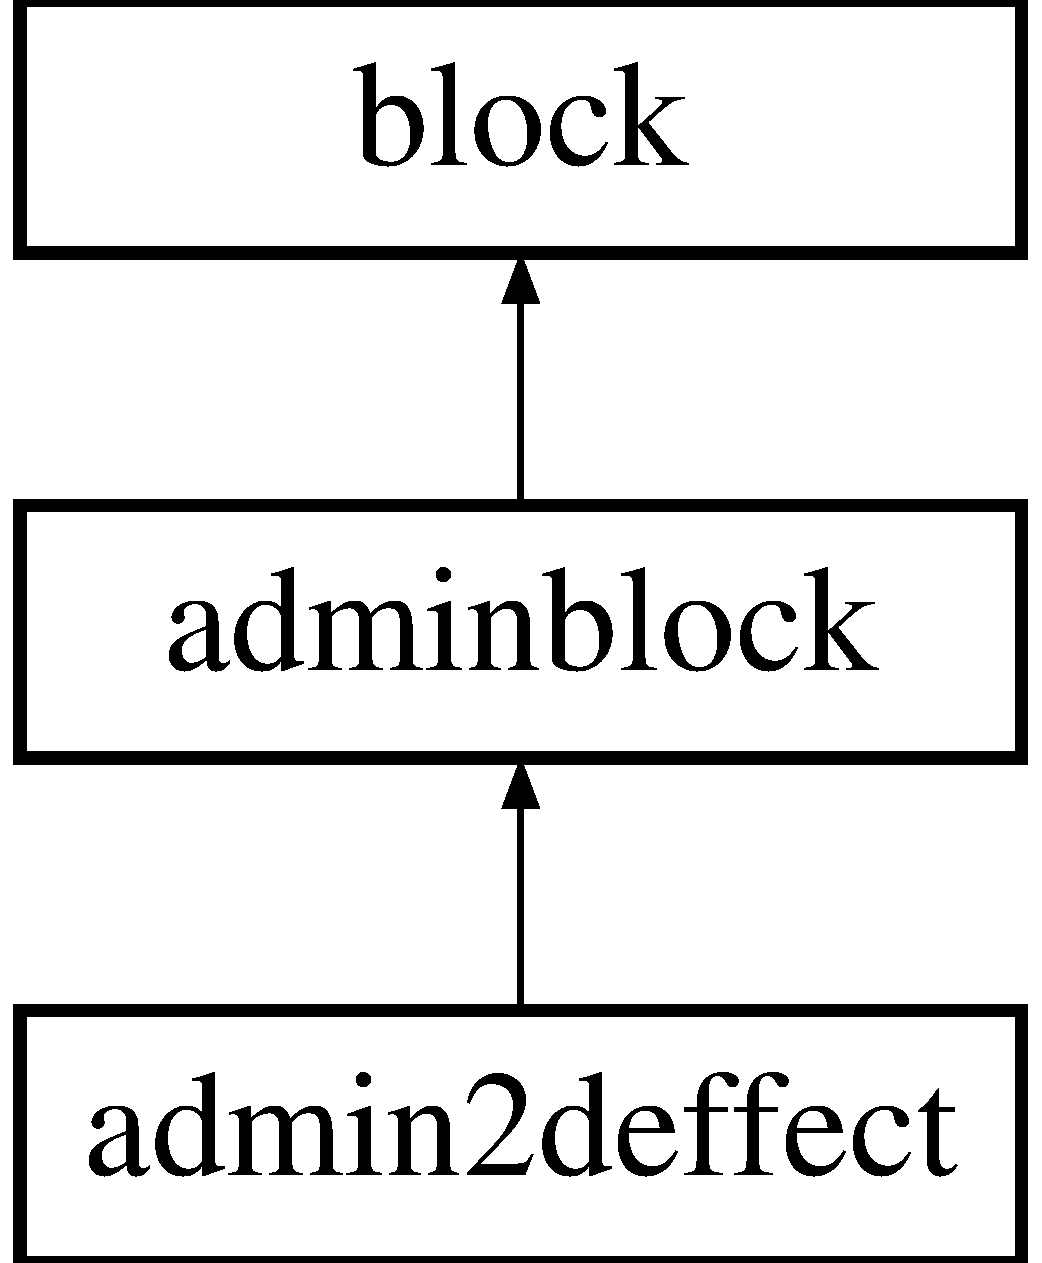
\includegraphics[height=3.000000cm]{classadmin2deffect}
\end{center}
\end{figure}
\subsection*{\-Métodos públicos}
\begin{DoxyCompactItemize}
\item 
\hypertarget{classadmin2deffect_a53778a0feb5e76953729f6d462a60a6d}{{\bfseries create\-Fields} ()}\label{classadmin2deffect_a53778a0feb5e76953729f6d462a60a6d}

\item 
\hypertarget{classadmin2deffect_ad419ce3181b153ff1ca5a3e9489d0d0c}{{\bfseries create\-Relations1\-N} ()}\label{classadmin2deffect_ad419ce3181b153ff1ca5a3e9489d0d0c}

\item 
\hypertarget{classadmin2deffect_a248fde2f295d2f474d17cdb8687db3e9}{{\bfseries create\-Relations1\-N1\-N} ()}\label{classadmin2deffect_a248fde2f295d2f474d17cdb8687db3e9}

\item 
\hypertarget{classadmin2deffect_aa7719143b1c8117347888897aa8e91de}{{\bfseries find\-Model\-Id} ()}\label{classadmin2deffect_aa7719143b1c8117347888897aa8e91de}

\end{DoxyCompactItemize}


\subsection{\-Descripción detallada}


\-Definición en la línea 5 del archivo admin2deffect.\-php.



\-La documentación para esta clase fue generada a partir del siguiente fichero\-:\begin{DoxyCompactItemize}
\item 
admin/admin2deffect.\-php\end{DoxyCompactItemize}

\hypertarget{classadminblock}{}\section{Referencia de la Clase adminblock}
\label{classadminblock}\index{adminblock@{adminblock}}
Diagrama de herencias de adminblock\begin{figure}[H]
\begin{center}
\leavevmode
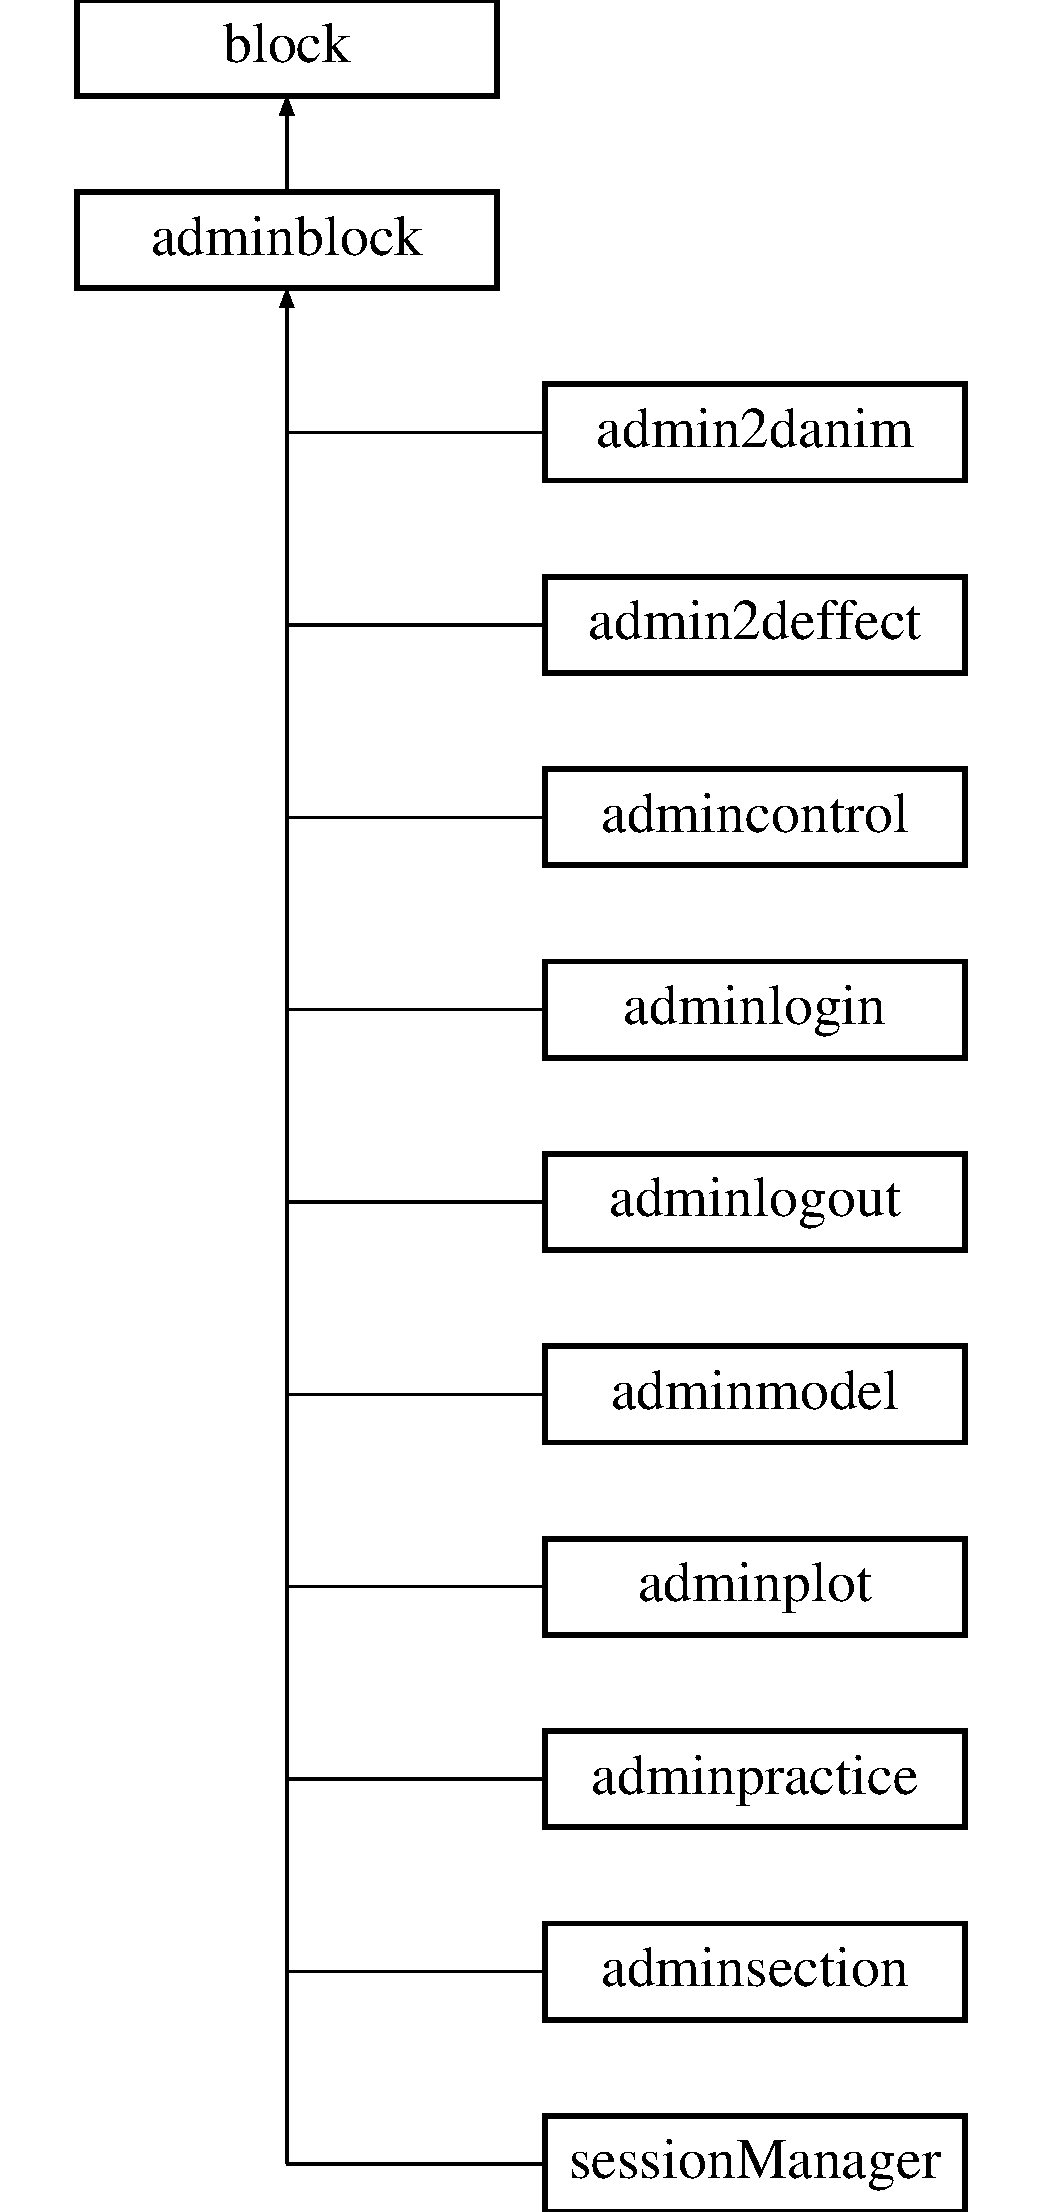
\includegraphics[height=12.000000cm]{classadminblock}
\end{center}
\end{figure}
\subsection*{Métodos públicos}
\begin{DoxyCompactItemize}
\item 
\mbox{\Hypertarget{classadminblock_a5a9c45c8bdb32b8cb34341c0651e8970}\label{classadminblock_a5a9c45c8bdb32b8cb34341c0651e8970}} 
{\bfseries select\+Section} (\$level, \$section\+\_\+sql, \$section\+\_\+id)
\item 
\mbox{\Hypertarget{classadminblock_a799a5af3e9759b2a1b6f110940fd03cf}\label{classadminblock_a799a5af3e9759b2a1b6f110940fd03cf}} 
{\bfseries select\+From\+Table} (\$table, \$model\+\_\+id, \$variable\+\_\+id)
\item 
\mbox{\Hypertarget{classadminblock_a37317b2ea7f1da508d561befcc232af7}\label{classadminblock_a37317b2ea7f1da508d561befcc232af7}} 
{\bfseries select\+Options} (\$F, \$id)
\item 
\mbox{\Hypertarget{classadminblock_ada80fd6066d96b488861e47485db043f}\label{classadminblock_ada80fd6066d96b488861e47485db043f}} 
{\bfseries display\+One\+Field} (\$data, \$F, \$class)
\item 
\mbox{\Hypertarget{classadminblock_a7bb1e8f357803f17830becbd417588ae}\label{classadminblock_a7bb1e8f357803f17830becbd417588ae}} 
{\bfseries display\+Fields} (\$data)
\item 
\mbox{\Hypertarget{classadminblock_a2aaea9bf7d5956dfb59322a7009b2538}\label{classadminblock_a2aaea9bf7d5956dfb59322a7009b2538}} 
{\bfseries update} ()
\item 
\mbox{\Hypertarget{classadminblock_ab7be1803fca03951754c864962aa072d}\label{classadminblock_ab7be1803fca03951754c864962aa072d}} 
{\bfseries update1\+N\+N1} ()
\item 
\mbox{\Hypertarget{classadminblock_a6c3808e99afabab0fb51663ea7a972a4}\label{classadminblock_a6c3808e99afabab0fb51663ea7a972a4}} 
{\bfseries insert} ()
\item 
\mbox{\Hypertarget{classadminblock_a85f955923111d4f0096b183a35bd10f2}\label{classadminblock_a85f955923111d4f0096b183a35bd10f2}} 
{\bfseries insert1\+N\+N1} ()
\item 
\mbox{\Hypertarget{classadminblock_a7951b7fba32a86503b434b99b926b16c}\label{classadminblock_a7951b7fba32a86503b434b99b926b16c}} 
{\bfseries delete} ()
\item 
\mbox{\Hypertarget{classadminblock_a410e2d751c1c7237f844d5e8f58e8fb6}\label{classadminblock_a410e2d751c1c7237f844d5e8f58e8fb6}} 
{\bfseries delete1\+N\+N1} ()
\item 
\mbox{\Hypertarget{classadminblock_a34b581b03da821f3729ee1ba01f43fdb}\label{classadminblock_a34b581b03da821f3729ee1ba01f43fdb}} 
{\bfseries create\+Relations1N} ()
\item 
\mbox{\Hypertarget{classadminblock_aede90fd2d786dd82337633d4db7e96f2}\label{classadminblock_aede90fd2d786dd82337633d4db7e96f2}} 
{\bfseries create\+Relations1\+N1N} ()
\item 
\mbox{\Hypertarget{classadminblock_ae33dcdb42cc7447da90720aa43de43dd}\label{classadminblock_ae33dcdb42cc7447da90720aa43de43dd}} 
{\bfseries create\+Relations1\+N\+N1} ()
\item 
\mbox{\Hypertarget{classadminblock_a3030ee20a0832cb36962eb61d1e54f1c}\label{classadminblock_a3030ee20a0832cb36962eb61d1e54f1c}} 
{\bfseries display\+Own} ()
\item 
\mbox{\Hypertarget{classadminblock_aedb5144f1e277464380c13f20dbd77e3}\label{classadminblock_aedb5144f1e277464380c13f20dbd77e3}} 
{\bfseries display\+One\+Relation1N} (\$rel)
\item 
\mbox{\Hypertarget{classadminblock_ae9f1ab4b65679f7ac9389b96aa5f09d9}\label{classadminblock_ae9f1ab4b65679f7ac9389b96aa5f09d9}} 
{\bfseries display\+Relations1N} ()
\item 
\mbox{\Hypertarget{classadminblock_a79090e871858d6fb698b50b193563de8}\label{classadminblock_a79090e871858d6fb698b50b193563de8}} 
{\bfseries display\+One\+Relation1\+N1N} (\$rel)
\item 
\mbox{\Hypertarget{classadminblock_a70b65d53f785e095f0e5266aaa0b3c87}\label{classadminblock_a70b65d53f785e095f0e5266aaa0b3c87}} 
{\bfseries display\+Relations1\+N1N} ()
\item 
\mbox{\Hypertarget{classadminblock_aca1a65edd3e33238a64ea979431e3e4b}\label{classadminblock_aca1a65edd3e33238a64ea979431e3e4b}} 
{\bfseries display\+One\+Relation1\+N\+N1} (\$rel)
\item 
\mbox{\Hypertarget{classadminblock_a8aa7529d8e7e8e8db8bd792eb5803852}\label{classadminblock_a8aa7529d8e7e8e8db8bd792eb5803852}} 
{\bfseries display\+Relations1\+N\+N1} ()
\item 
\mbox{\Hypertarget{classadminblock_aa65d7b380b388ce3f6269b3b2bd1f640}\label{classadminblock_aa65d7b380b388ce3f6269b3b2bd1f640}} 
{\bfseries create\+Fields\+And\+Relations} ()
\item 
\mbox{\Hypertarget{classadminblock_a9f67e700a2b2002b4985118de36a10f3}\label{classadminblock_a9f67e700a2b2002b4985118de36a10f3}} 
{\bfseries display\+Post\+Own} ()
\item 
\mbox{\Hypertarget{classadminblock_ac5a1c7c515e5e60b07092ecb37515c73}\label{classadminblock_ac5a1c7c515e5e60b07092ecb37515c73}} 
{\bfseries display\+All} ()
\item 
\mbox{\Hypertarget{classadminblock_a1823f78aa77cbf1e12b631ce5adae860}\label{classadminblock_a1823f78aa77cbf1e12b631ce5adae860}} 
{\bfseries display} ()
\end{DoxyCompactItemize}
\subsection*{Atributos públicos}
\begin{DoxyCompactItemize}
\item 
\mbox{\Hypertarget{classadminblock_a86efd09cdc94c3fdaa3b5abbfc74fbef}\label{classadminblock_a86efd09cdc94c3fdaa3b5abbfc74fbef}} 
{\bfseries \$fields}
\item 
\mbox{\Hypertarget{classadminblock_aff6ad656e948f5a333e940e59cc923b2}\label{classadminblock_aff6ad656e948f5a333e940e59cc923b2}} 
{\bfseries \$table}
\item 
\mbox{\Hypertarget{classadminblock_a65a19960858ea506655592cb1fc5bb0e}\label{classadminblock_a65a19960858ea506655592cb1fc5bb0e}} 
{\bfseries \$sectionidname}
\item 
\mbox{\Hypertarget{classadminblock_a61b563c0dfeec8a659713b5db1ac3b0b}\label{classadminblock_a61b563c0dfeec8a659713b5db1ac3b0b}} 
{\bfseries \$idname}
\item 
\mbox{\Hypertarget{classadminblock_a193ac3c47d509ca1464480c73b7dac7b}\label{classadminblock_a193ac3c47d509ca1464480c73b7dac7b}} 
{\bfseries \$idvalue}
\item 
\mbox{\Hypertarget{classadminblock_a114998a4cea5bc508c8787af12f525ed}\label{classadminblock_a114998a4cea5bc508c8787af12f525ed}} 
{\bfseries \$blockname}
\item 
\mbox{\Hypertarget{classadminblock_a8aff2f80ea6041741f0aff93b5f86e3e}\label{classadminblock_a8aff2f80ea6041741f0aff93b5f86e3e}} 
{\bfseries \$relations1N}
\item 
\mbox{\Hypertarget{classadminblock_a4da890b0eaa88cf3c3214ea4cb0c2d9c}\label{classadminblock_a4da890b0eaa88cf3c3214ea4cb0c2d9c}} 
{\bfseries \$relations1\+N1N}
\item 
\mbox{\Hypertarget{classadminblock_a92be1741e34afc7c85f574e557b4fca2}\label{classadminblock_a92be1741e34afc7c85f574e557b4fca2}} 
{\bfseries \$relations1\+N\+N1}
\end{DoxyCompactItemize}


\subsection{Descripción detallada}


Definición en la línea 5 del archivo adminblock.\+php.



La documentación para esta clase fue generada a partir del siguiente fichero\+:\begin{DoxyCompactItemize}
\item 
/home/ogduartev/public\+\_\+html/unvl-\/\+Git\+Hub/\+U\+N\+Virtual\+Lab/admin/adminblock.\+php\end{DoxyCompactItemize}

\hypertarget{classadmincontrol}{\section{\-Referencia de la \-Clase admincontrol}
\label{classadmincontrol}\index{admincontrol@{admincontrol}}
}
\-Diagrama de herencias de admincontrol\begin{figure}[H]
\begin{center}
\leavevmode
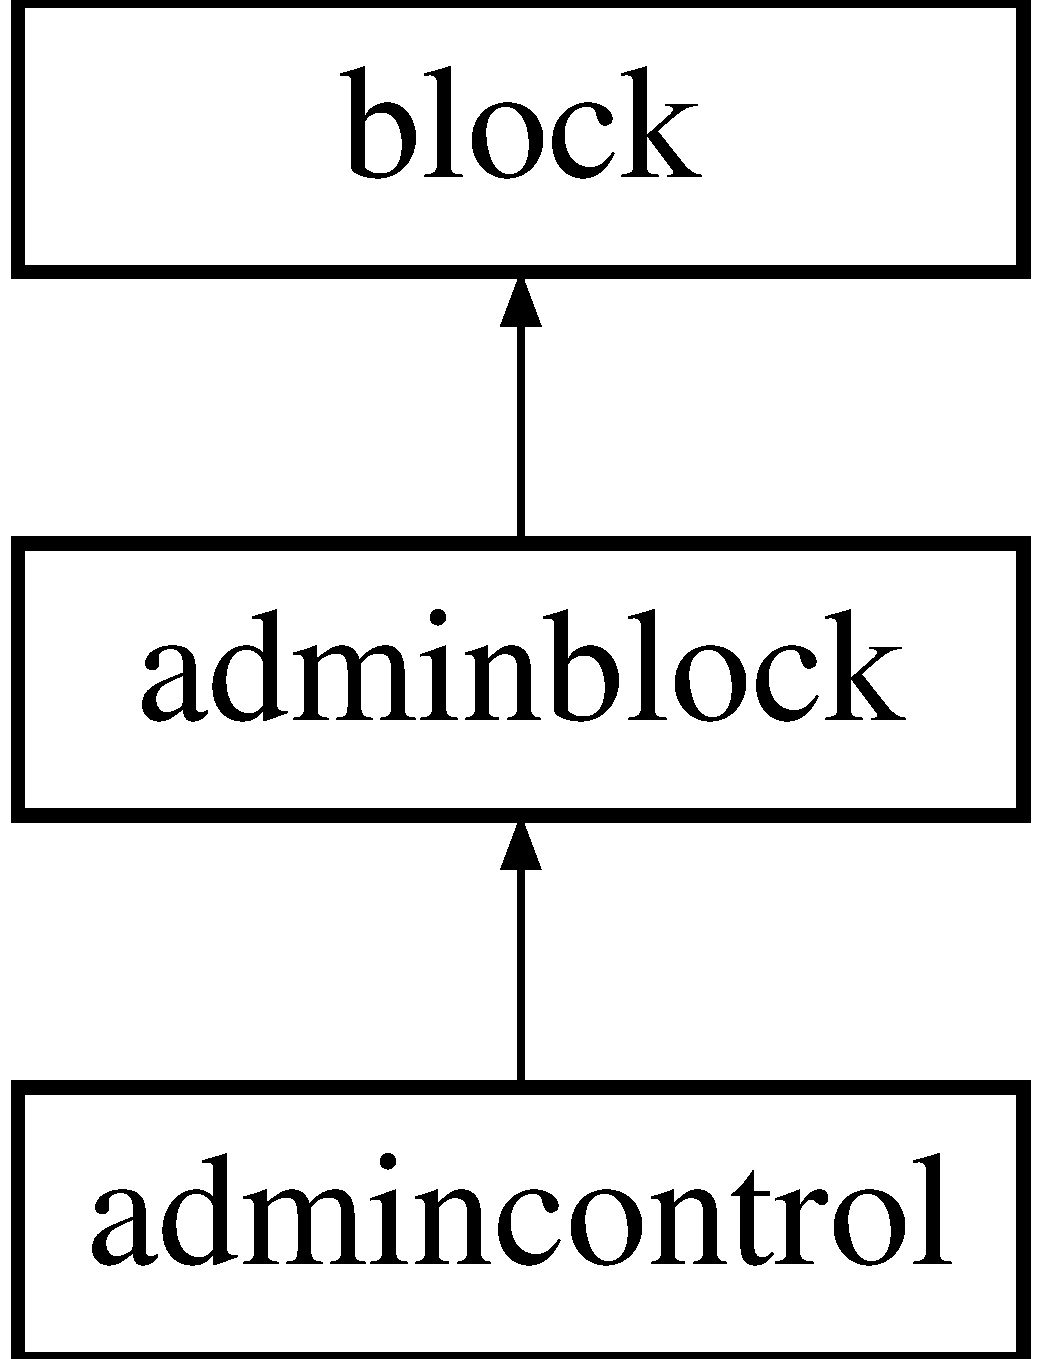
\includegraphics[height=3.000000cm]{classadmincontrol}
\end{center}
\end{figure}
\subsection*{\-Métodos públicos}
\begin{DoxyCompactItemize}
\item 
\hypertarget{classadmincontrol_a105d0b8037931db4a31acb5eb35db838}{{\bfseries create\-Fields} ()}\label{classadmincontrol_a105d0b8037931db4a31acb5eb35db838}

\item 
\hypertarget{classadmincontrol_a678192be99fa0eddbe86d999e9d573f2}{{\bfseries create\-Relations1\-N1\-N} ()}\label{classadmincontrol_a678192be99fa0eddbe86d999e9d573f2}

\item 
\hypertarget{classadmincontrol_a375df9422444a3312a77931d41e7c565}{{\bfseries find\-Model\-Id} ()}\label{classadmincontrol_a375df9422444a3312a77931d41e7c565}

\item 
\hypertarget{classadmincontrol_a8996c04e21d903aca9ad406b6d274aba}{{\bfseries update} ()}\label{classadmincontrol_a8996c04e21d903aca9ad406b6d274aba}

\end{DoxyCompactItemize}


\subsection{\-Descripción detallada}


\-Definición en la línea 4 del archivo admincontrol.\-php.



\-La documentación para esta clase fue generada a partir del siguiente fichero\-:\begin{DoxyCompactItemize}
\item 
admin/admincontrol.\-php\end{DoxyCompactItemize}

\hypertarget{classadminlogin}{\section{\-Referencia de la \-Clase adminlogin}
\label{classadminlogin}\index{adminlogin@{adminlogin}}
}
\-Diagrama de herencias de adminlogin\begin{figure}[H]
\begin{center}
\leavevmode
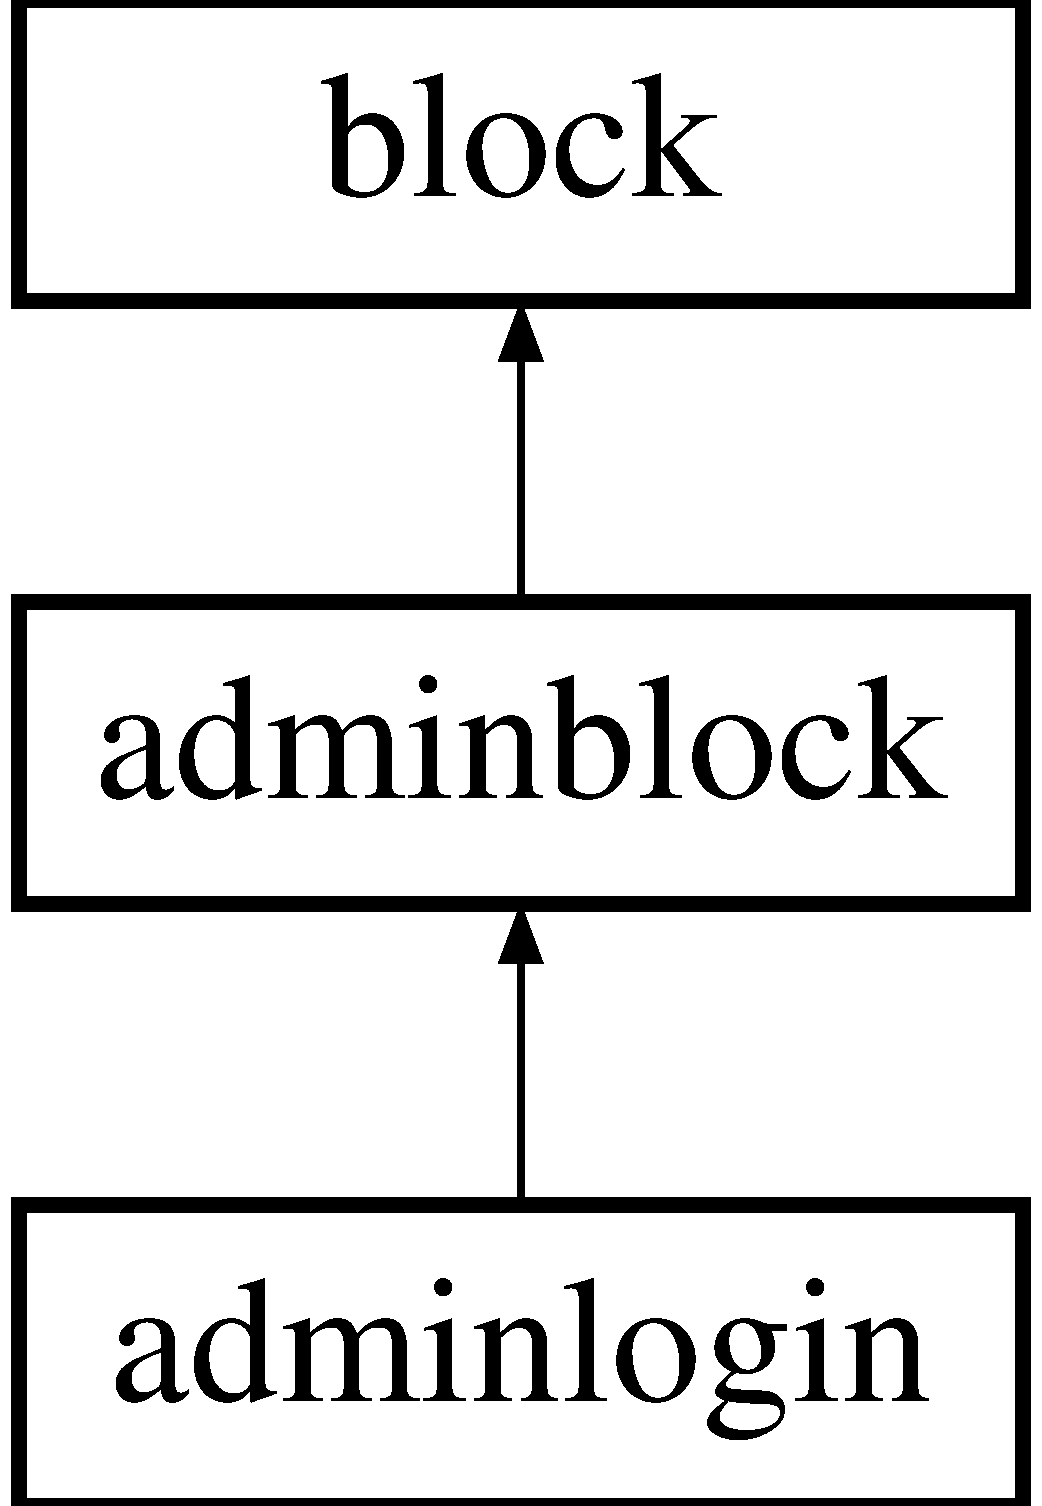
\includegraphics[height=3.000000cm]{classadminlogin}
\end{center}
\end{figure}
\subsection*{\-Métodos públicos}
\begin{DoxyCompactItemize}
\item 
\hypertarget{classadminlogin_a9413fd10c23ace3cca43c2a4919b5941}{{\bfseries show\-Message} ()}\label{classadminlogin_a9413fd10c23ace3cca43c2a4919b5941}

\item 
\hypertarget{classadminlogin_a0b0d46370f41b7d49727d69d404f7eb3}{{\bfseries show\-Buttons} ()}\label{classadminlogin_a0b0d46370f41b7d49727d69d404f7eb3}

\item 
\hypertarget{classadminlogin_a7133dff5753a8101111b6e3d4e2d6959}{{\bfseries display} ()}\label{classadminlogin_a7133dff5753a8101111b6e3d4e2d6959}

\end{DoxyCompactItemize}


\subsection{\-Descripción detallada}


\-Definición en la línea 4 del archivo adminlogin.\-php.



\-La documentación para esta clase fue generada a partir del siguiente fichero\-:\begin{DoxyCompactItemize}
\item 
admin/adminlogin.\-php\end{DoxyCompactItemize}

\hypertarget{classadminlogout}{}\section{Referencia de la Clase adminlogout}
\label{classadminlogout}\index{adminlogout@{adminlogout}}
Diagrama de herencias de adminlogout\begin{figure}[H]
\begin{center}
\leavevmode
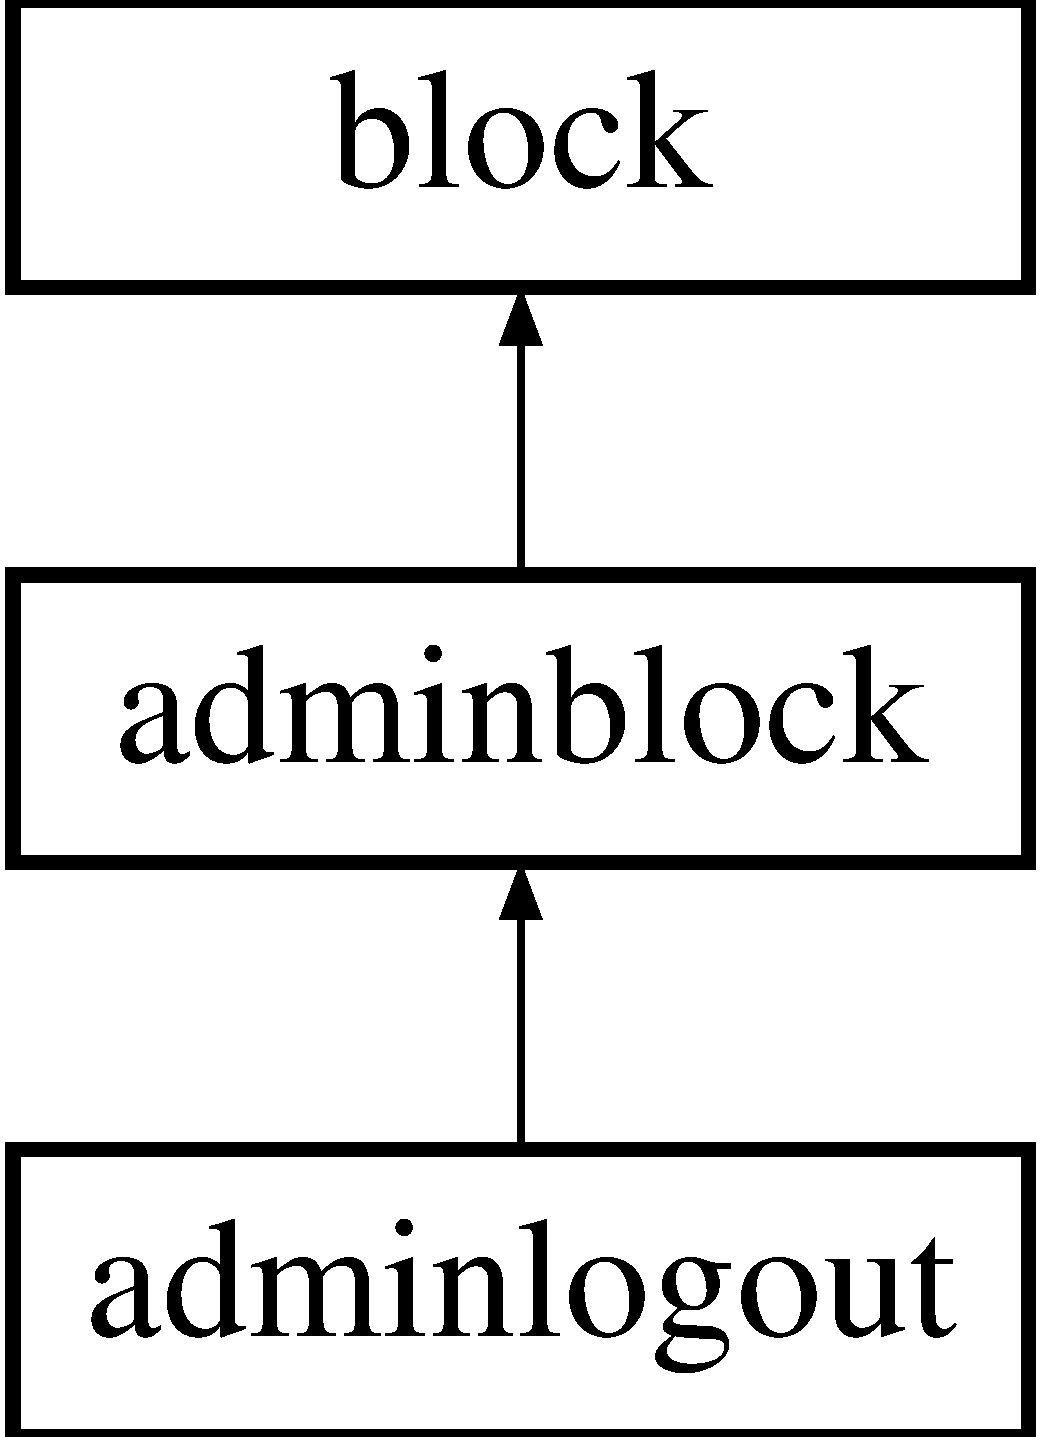
\includegraphics[height=3.000000cm]{classadminlogout}
\end{center}
\end{figure}
\subsection*{Métodos públicos}
\begin{DoxyCompactItemize}
\item 
\mbox{\Hypertarget{classadminlogout_a75f9b062b4c8cd673c544a0c2ce62034}\label{classadminlogout_a75f9b062b4c8cd673c544a0c2ce62034}} 
{\bfseries display} ()
\end{DoxyCompactItemize}
\subsection*{Otros miembros heredados}


\subsection{Descripción detallada}


Definición en la línea 4 del archivo adminlogout.\+php.



La documentación para esta clase fue generada a partir del siguiente fichero\+:\begin{DoxyCompactItemize}
\item 
/home/ogduartev/public\+\_\+html/unvl-\/\+Git\+Hub/\+U\+N\+Virtual\+Lab/admin/adminlogout.\+php\end{DoxyCompactItemize}

\hypertarget{classadminmodel}{}\section{Referencia de la Clase adminmodel}
\label{classadminmodel}\index{adminmodel@{adminmodel}}
Diagrama de herencias de adminmodel\begin{figure}[H]
\begin{center}
\leavevmode
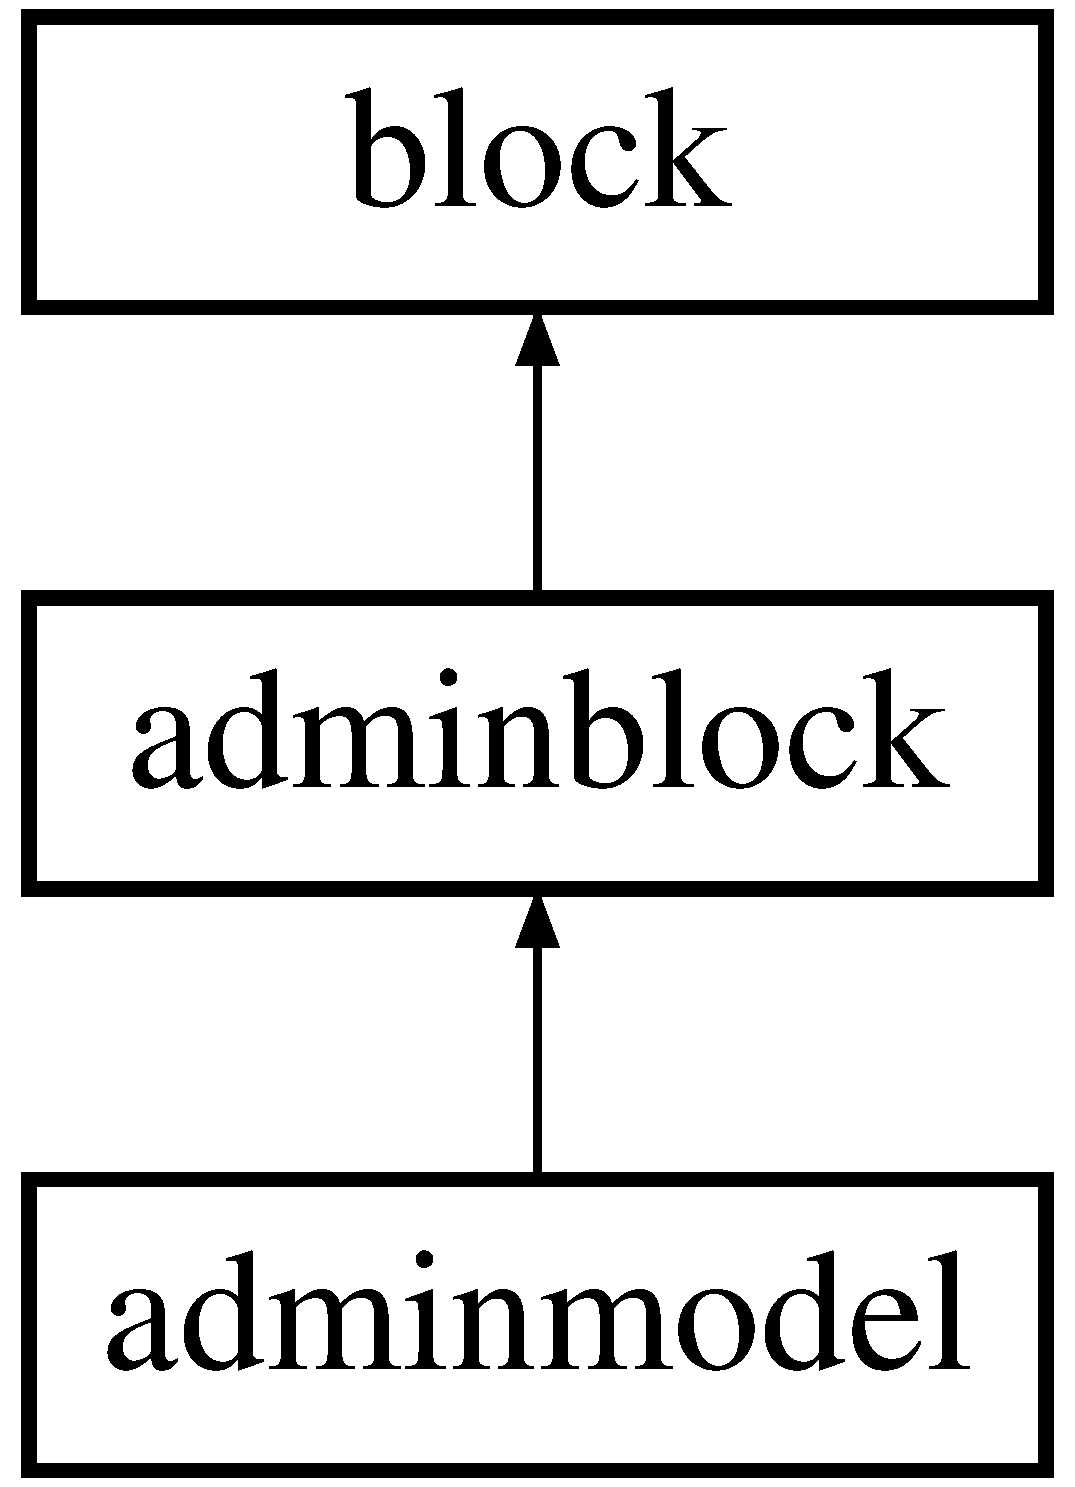
\includegraphics[height=3.000000cm]{classadminmodel}
\end{center}
\end{figure}
\subsection*{Métodos públicos}
\begin{DoxyCompactItemize}
\item 
\mbox{\Hypertarget{classadminmodel_a719d03fccd7778a3c34d485544ba60e3}\label{classadminmodel_a719d03fccd7778a3c34d485544ba60e3}} 
{\bfseries create\+Fields} ()
\item 
\mbox{\Hypertarget{classadminmodel_ae6097b00d7e11027b2de92b9da9eaa92}\label{classadminmodel_ae6097b00d7e11027b2de92b9da9eaa92}} 
{\bfseries create\+Relations1N} ()
\item 
\mbox{\Hypertarget{classadminmodel_afb87584c89afa1378abe6c72c54591a3}\label{classadminmodel_afb87584c89afa1378abe6c72c54591a3}} 
{\bfseries create\+Relations1\+N\+N1} ()
\end{DoxyCompactItemize}
\subsection*{Otros miembros heredados}


\subsection{Descripción detallada}


Definición en la línea 4 del archivo adminmodel.\+php.



La documentación para esta clase fue generada a partir del siguiente fichero\+:\begin{DoxyCompactItemize}
\item 
/home/ogduartev/public\+\_\+html/unvl-\/\+Git\+Hub/\+U\+N\+Virtual\+Lab/admin/adminmodel.\+php\end{DoxyCompactItemize}

\hypertarget{classadminmodelfiles}{\section{\-Referencia de la \-Clase adminmodelfiles}
\label{classadminmodelfiles}\index{adminmodelfiles@{adminmodelfiles}}
}
\-Diagrama de herencias de adminmodelfiles\begin{figure}[H]
\begin{center}
\leavevmode
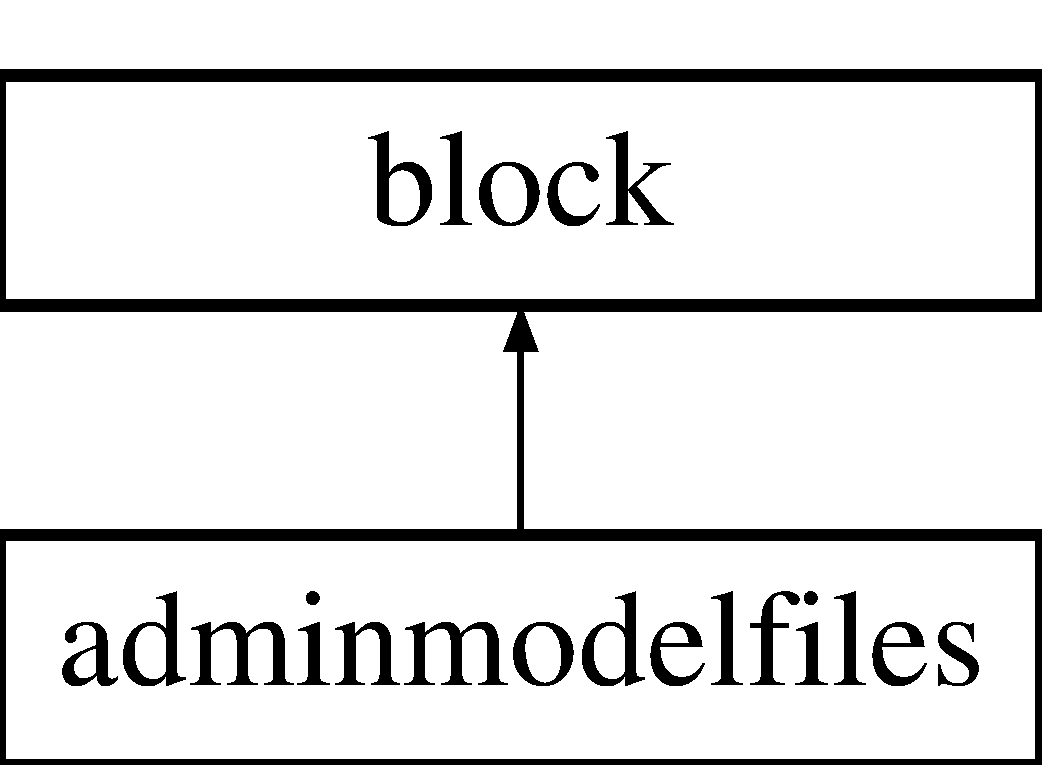
\includegraphics[height=2.000000cm]{classadminmodelfiles}
\end{center}
\end{figure}
\subsection*{\-Métodos públicos}
\begin{DoxyCompactItemize}
\item 
\hypertarget{classadminmodelfiles_ab2909af33bf70f8cdec68680ab98b0b0}{{\bfseries createdata} ()}\label{classadminmodelfiles_ab2909af33bf70f8cdec68680ab98b0b0}

\item 
\hypertarget{classadminmodelfiles_a11f958e22ba2d5ef27a4ea03314b11b4}{{\bfseries copyfile} (\$\-F\-I\-L\-E, \$\-F\-D)}\label{classadminmodelfiles_a11f958e22ba2d5ef27a4ea03314b11b4}

\item 
\hypertarget{classadminmodelfiles_a200364be0dce2f68d1d8641766323d63}{{\bfseries db\-\_\-modelica} (\$\-F\-I\-L\-E, \$\-F\-D)}\label{classadminmodelfiles_a200364be0dce2f68d1d8641766323d63}

\item 
\hypertarget{classadminmodelfiles_a257dbbccb35194e4a143a335407cd501}{{\bfseries db\-\_\-documentation} (\$\-F\-I\-L\-E, \$\-F\-D)}\label{classadminmodelfiles_a257dbbccb35194e4a143a335407cd501}

\item 
\hypertarget{classadminmodelfiles_a3c37216d53bf9ad26c522eaed996514e}{{\bfseries compile} (\$\-F\-D)}\label{classadminmodelfiles_a3c37216d53bf9ad26c522eaed996514e}

\item 
\hypertarget{classadminmodelfiles_a5084adb76dcf35dc888280a7312014b9}{{\bfseries db\-\_\-executable} (\$\-F\-I\-L\-E, \$\-F\-D)}\label{classadminmodelfiles_a5084adb76dcf35dc888280a7312014b9}

\item 
\hypertarget{classadminmodelfiles_afa448154eccb7ec943cf393dfa542241}{{\bfseries read\-Init\-Xml} (\$fn)}\label{classadminmodelfiles_afa448154eccb7ec943cf393dfa542241}

\item 
\hypertarget{classadminmodelfiles_aa8e22f2bb6f92bcf8c62e2df207bc262}{{\bfseries vars\-In\-Init\-Xml} (\$fn)}\label{classadminmodelfiles_aa8e22f2bb6f92bcf8c62e2df207bc262}

\item 
\hypertarget{classadminmodelfiles_af51f1e4ae2b589ed8bb4bdc7d97111ae}{{\bfseries vars\-In\-Res\-Csv} (\$fn)}\label{classadminmodelfiles_af51f1e4ae2b589ed8bb4bdc7d97111ae}

\item 
\hypertarget{classadminmodelfiles_a9bed418a7e4ae7f28480ab6cf9767ea7}{{\bfseries in\-D\-B} (\$\-Table)}\label{classadminmodelfiles_a9bed418a7e4ae7f28480ab6cf9767ea7}

\item 
\hypertarget{classadminmodelfiles_a9ded5ca54c1ed7fe34cc831224576918}{{\bfseries update\-D\-Bvars\-And\-Pars} (\$fn)}\label{classadminmodelfiles_a9ded5ca54c1ed7fe34cc831224576918}

\item 
\hypertarget{classadminmodelfiles_aa36b9b08512d363174d08c8711576c3a}{{\bfseries compare\-Update\-X\-M\-L\-D\-B} (\$\-Xml, \$\-Table)}\label{classadminmodelfiles_aa36b9b08512d363174d08c8711576c3a}

\item 
\hypertarget{classadminmodelfiles_a75b3c881bbfa514acd88bc32597cba84}{{\bfseries upload} ()}\label{classadminmodelfiles_a75b3c881bbfa514acd88bc32597cba84}

\item 
\hypertarget{classadminmodelfiles_acd1759b4b15d819f14316280f3f87c29}{{\bfseries display\-F\-D} (\$\-F\-D)}\label{classadminmodelfiles_acd1759b4b15d819f14316280f3f87c29}

\item 
\hypertarget{classadminmodelfiles_a9aeb4f143fd7967234ac65e070baff8a}{{\bfseries display} ()}\label{classadminmodelfiles_a9aeb4f143fd7967234ac65e070baff8a}

\end{DoxyCompactItemize}
\subsection*{\-Atributos públicos}
\begin{DoxyCompactItemize}
\item 
\hypertarget{classadminmodelfiles_ac58f67d34dfa2c233883023b3787ead0}{{\bfseries \$filedata}}\label{classadminmodelfiles_ac58f67d34dfa2c233883023b3787ead0}

\end{DoxyCompactItemize}


\subsection{\-Descripción detallada}


\-Definición en la línea 4 del archivo adminmodelfiles.\-php.



\-La documentación para esta clase fue generada a partir del siguiente fichero\-:\begin{DoxyCompactItemize}
\item 
admin/adminmodelfiles.\-php\end{DoxyCompactItemize}

\hypertarget{classadminplot}{\section{\-Referencia de la \-Clase adminplot}
\label{classadminplot}\index{adminplot@{adminplot}}
}
\-Diagrama de herencias de adminplot\begin{figure}[H]
\begin{center}
\leavevmode
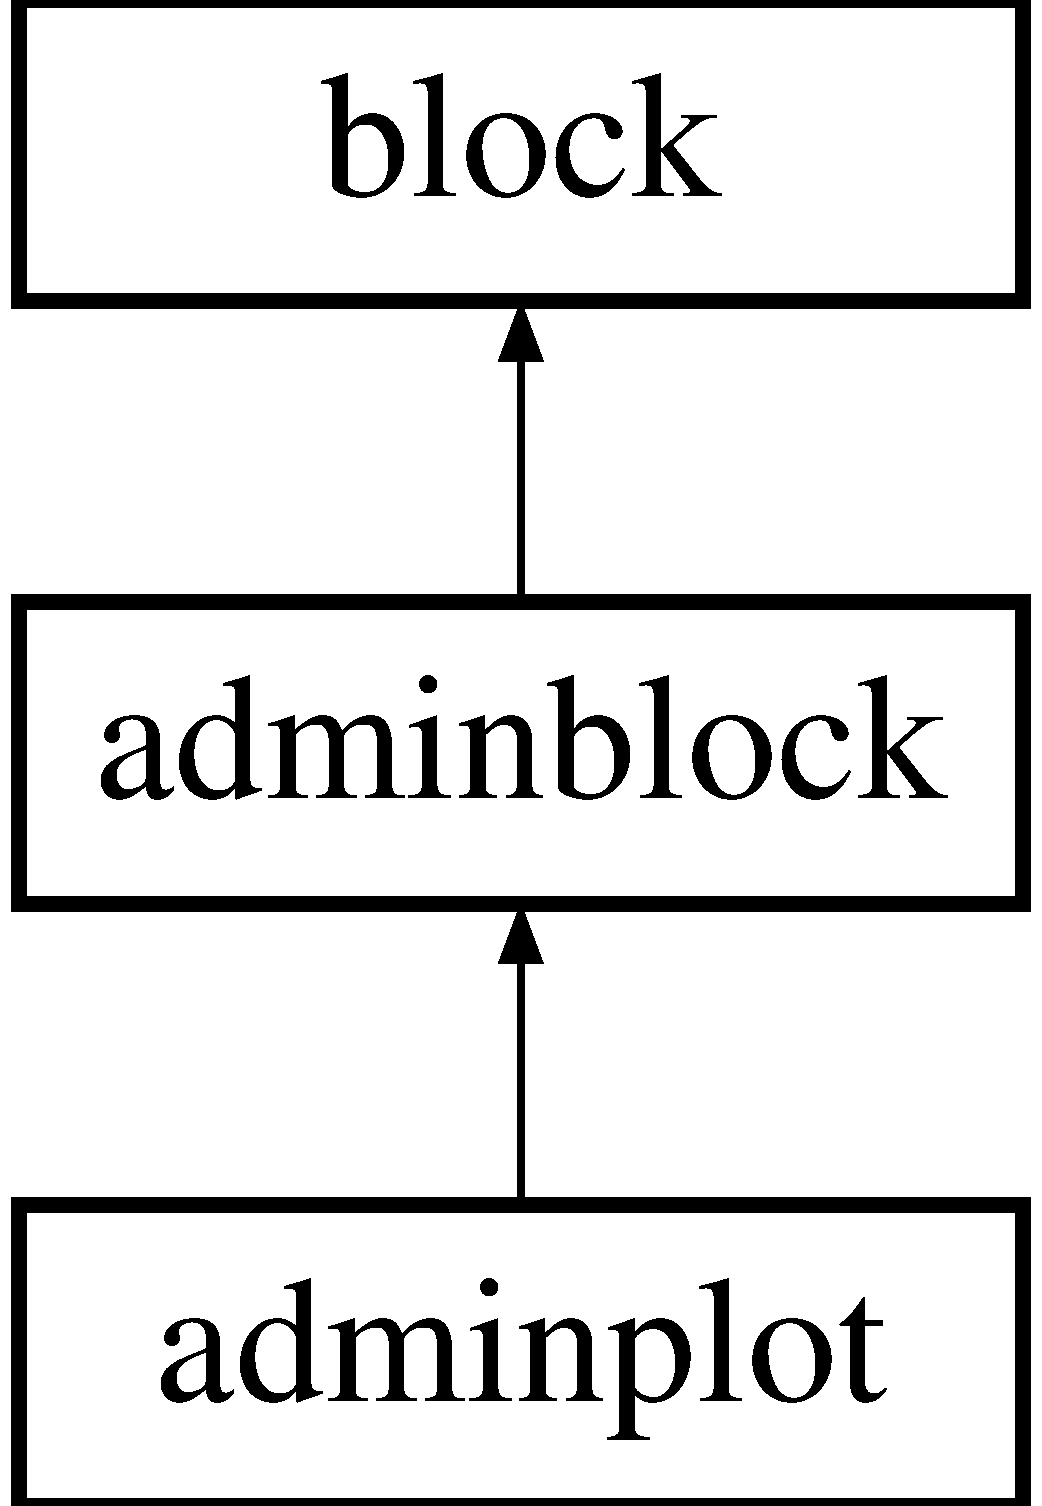
\includegraphics[height=3.000000cm]{classadminplot}
\end{center}
\end{figure}
\subsection*{\-Métodos públicos}
\begin{DoxyCompactItemize}
\item 
\hypertarget{classadminplot_a2a2a481056d85edf385da065689e1e00}{{\bfseries create\-Fields} ()}\label{classadminplot_a2a2a481056d85edf385da065689e1e00}

\item 
\hypertarget{classadminplot_a76a67aa739701746ba1d7e9ebf188b8b}{{\bfseries create\-Relations1\-N1\-N} ()}\label{classadminplot_a76a67aa739701746ba1d7e9ebf188b8b}

\item 
\hypertarget{classadminplot_a93304fb59e227ce3ec988112c1e94b03}{{\bfseries find\-Model\-Id} ()}\label{classadminplot_a93304fb59e227ce3ec988112c1e94b03}

\item 
\hypertarget{classadminplot_a3c9246442bd29d4c94d4df518eaafc05}{{\bfseries find\-Autoscale} (\$axis)}\label{classadminplot_a3c9246442bd29d4c94d4df518eaafc05}

\item 
\hypertarget{classadminplot_a7243383e1e65657bca4dd7e67d2fed48}{{\bfseries display\-Post\-Own} ()}\label{classadminplot_a7243383e1e65657bca4dd7e67d2fed48}

\item 
\hypertarget{classadminplot_a14ecb192e537e9861090cb2981dd5324}{{\bfseries display\-Plot} ()}\label{classadminplot_a14ecb192e537e9861090cb2981dd5324}

\item 
\hypertarget{classadminplot_adfbbf378d38bc707699a398dd35ea2ac}{{\bfseries update} ()}\label{classadminplot_adfbbf378d38bc707699a398dd35ea2ac}

\end{DoxyCompactItemize}


\subsection{\-Descripción detallada}


\-Definición en la línea 5 del archivo adminplot.\-php.



\-La documentación para esta clase fue generada a partir del siguiente fichero\-:\begin{DoxyCompactItemize}
\item 
admin/adminplot.\-php\end{DoxyCompactItemize}

\hypertarget{classadminpractice}{}\section{Referencia de la Clase adminpractice}
\label{classadminpractice}\index{adminpractice@{adminpractice}}
Diagrama de herencias de adminpractice\begin{figure}[H]
\begin{center}
\leavevmode
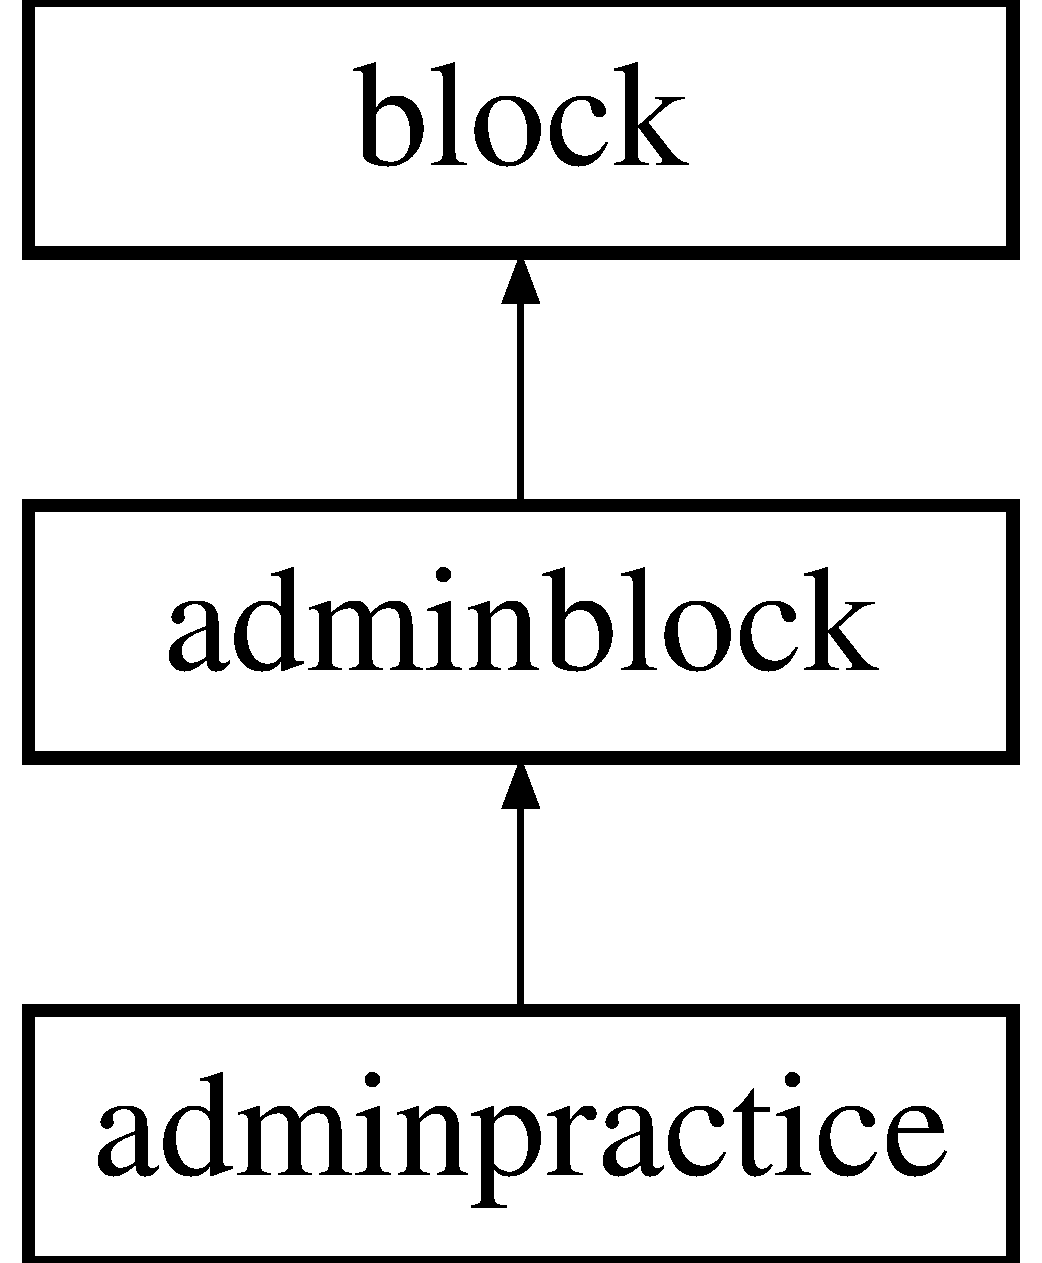
\includegraphics[height=3.000000cm]{classadminpractice}
\end{center}
\end{figure}
\subsection*{Métodos públicos}
\begin{DoxyCompactItemize}
\item 
\mbox{\Hypertarget{classadminpractice_a515878cf8a80e619382e2b0e142353db}\label{classadminpractice_a515878cf8a80e619382e2b0e142353db}} 
{\bfseries create\+Fields} ()
\end{DoxyCompactItemize}
\subsection*{Otros miembros heredados}


\subsection{Descripción detallada}


Definición en la línea 4 del archivo adminpractice.\+php.



La documentación para esta clase fue generada a partir del siguiente fichero\+:\begin{DoxyCompactItemize}
\item 
/home/ogduartev/public\+\_\+html/unvl-\/\+Git\+Hub/\+U\+N\+Virtual\+Lab/admin/adminpractice.\+php\end{DoxyCompactItemize}

\hypertarget{classadminsection}{}\section{Referencia de la Clase adminsection}
\label{classadminsection}\index{adminsection@{adminsection}}
Diagrama de herencias de adminsection\begin{figure}[H]
\begin{center}
\leavevmode
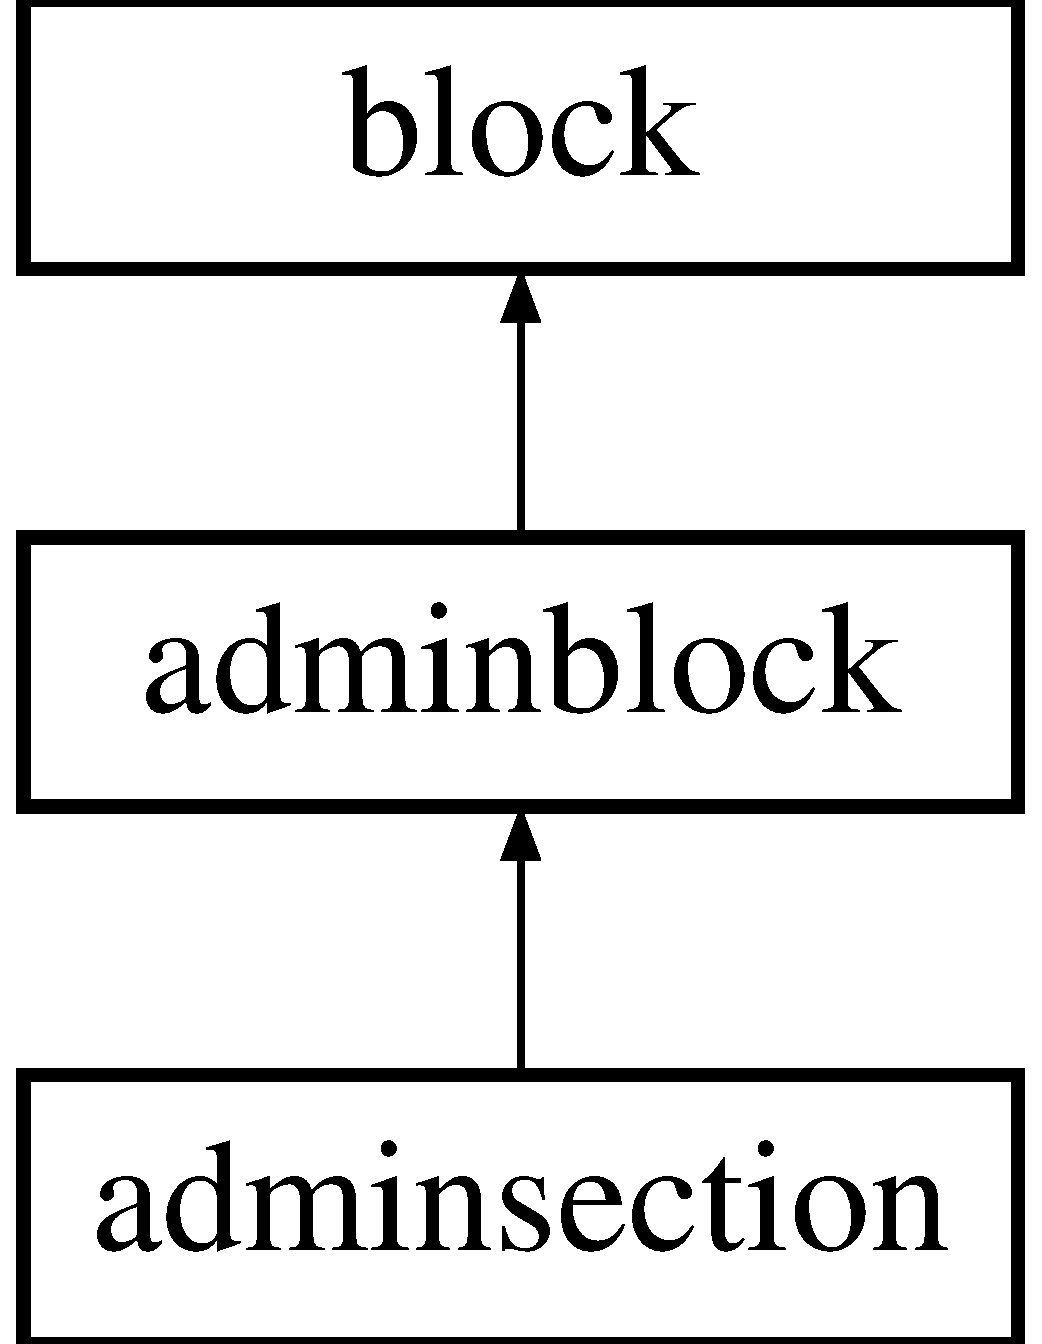
\includegraphics[height=3.000000cm]{classadminsection}
\end{center}
\end{figure}
\subsection*{Métodos públicos}
\begin{DoxyCompactItemize}
\item 
\mbox{\Hypertarget{classadminsection_a0a7554bf943204d3ff77514ea9f1a46c}\label{classadminsection_a0a7554bf943204d3ff77514ea9f1a46c}} 
{\bfseries create\+Fields} ()
\item 
\mbox{\Hypertarget{classadminsection_af74be6a7666ed8b360ed86f193a96e33}\label{classadminsection_af74be6a7666ed8b360ed86f193a96e33}} 
{\bfseries create\+Relations1N} ()
\end{DoxyCompactItemize}
\subsection*{Otros miembros heredados}


\subsection{Descripción detallada}


Definición en la línea 4 del archivo adminsection.\+php.



La documentación para esta clase fue generada a partir del siguiente fichero\+:\begin{DoxyCompactItemize}
\item 
/home/ogduartev/public\+\_\+html/unvl-\/\+Git\+Hub/\+U\+N\+Virtual\+Lab/admin/adminsection.\+php\end{DoxyCompactItemize}

\hypertarget{classanim2d}{\section{\-Referencia de la \-Clase anim2d}
\label{classanim2d}\index{anim2d@{anim2d}}
}
\-Diagrama de herencias de anim2d\begin{figure}[H]
\begin{center}
\leavevmode
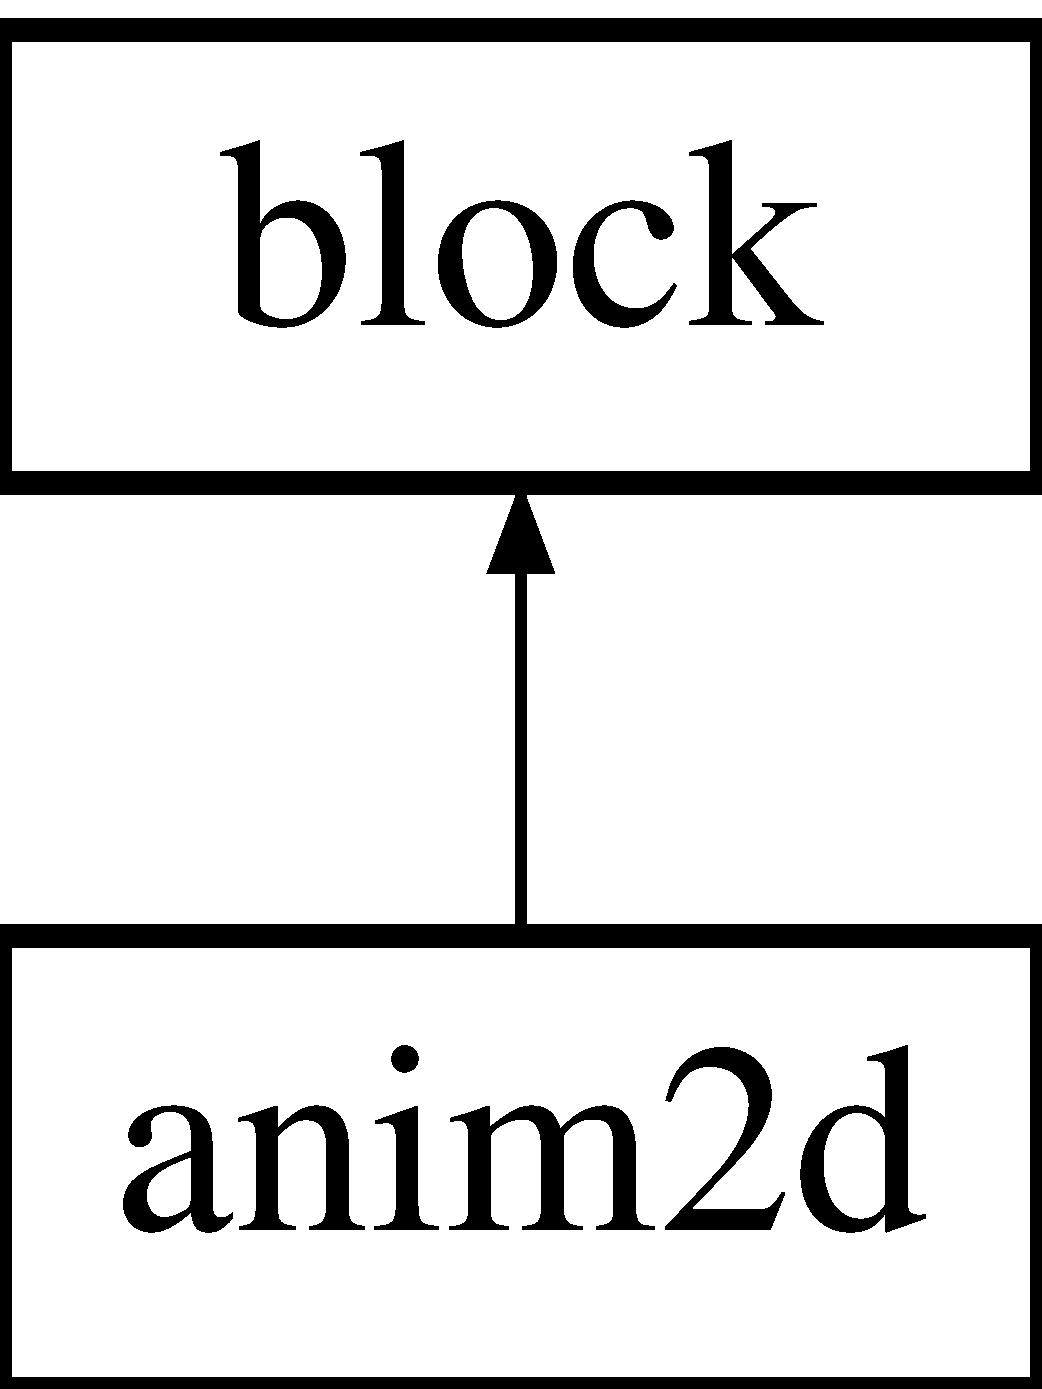
\includegraphics[height=2.000000cm]{classanim2d}
\end{center}
\end{figure}
\subsection*{\-Métodos públicos}
\begin{DoxyCompactItemize}
\item 
\hypertarget{classanim2d_a790ab010b1ab2211bf6fcbd8312b311c}{{\bfseries display\-Anim2d} (\$animation2d)}\label{classanim2d_a790ab010b1ab2211bf6fcbd8312b311c}

\item 
\hypertarget{classanim2d_ac75636f962552bb25edd7e31e8c8a07c}{{\bfseries display} ()}\label{classanim2d_ac75636f962552bb25edd7e31e8c8a07c}

\end{DoxyCompactItemize}


\subsection{\-Descripción detallada}


\-Definición en la línea 6 del archivo anim2d.\-php.



\-La documentación para esta clase fue generada a partir del siguiente fichero\-:\begin{DoxyCompactItemize}
\item 
anim2d.\-php\end{DoxyCompactItemize}

\hypertarget{classanimation2dSVG}{}\section{Referencia de la Clase animation2d\+S\+VG}
\label{classanimation2dSVG}\index{animation2d\+S\+VG@{animation2d\+S\+VG}}
Diagrama de herencias de animation2d\+S\+VG\begin{figure}[H]
\begin{center}
\leavevmode
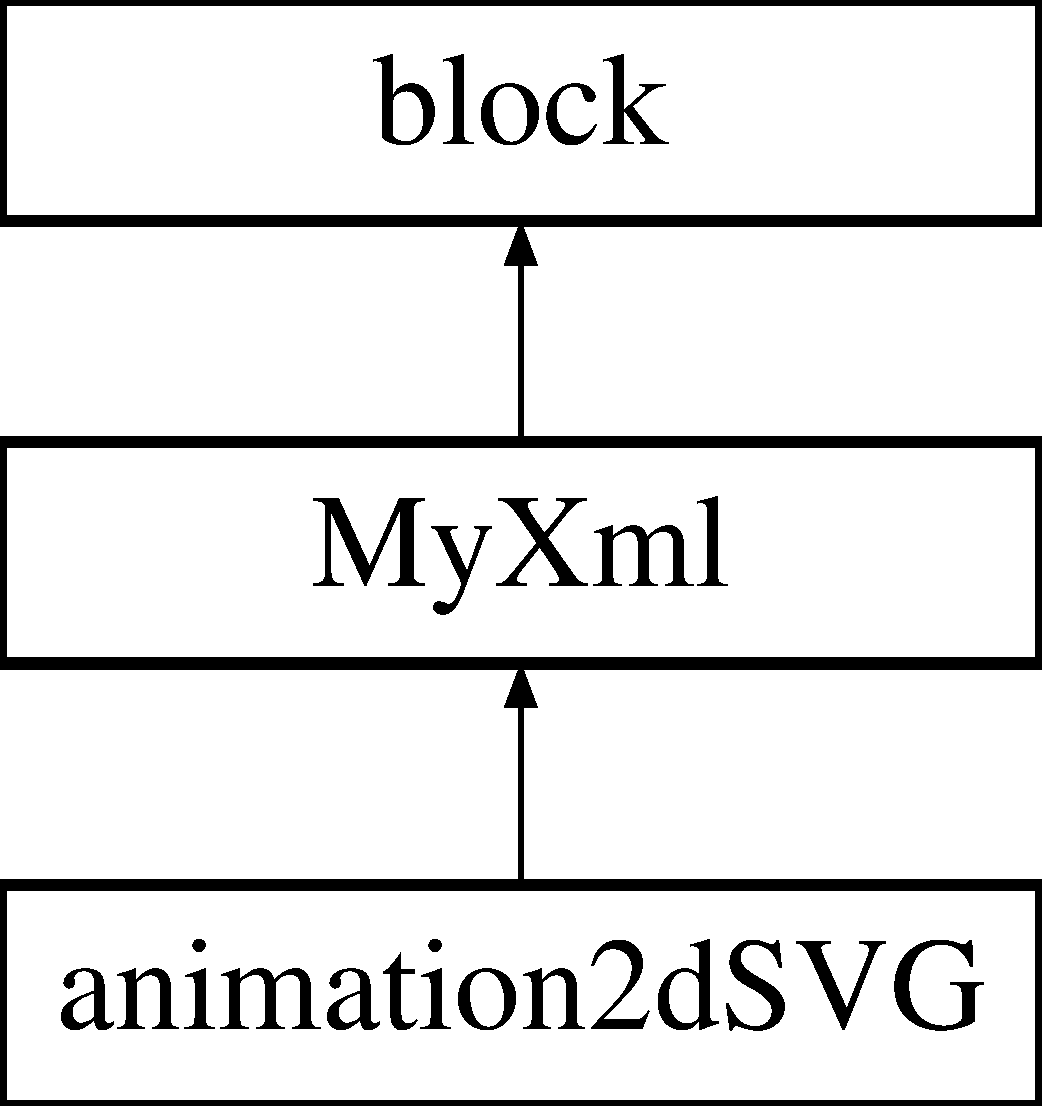
\includegraphics[height=3.000000cm]{classanimation2dSVG}
\end{center}
\end{figure}
\subsection*{Métodos públicos}
\begin{DoxyCompactItemize}
\item 
\mbox{\Hypertarget{classanimation2dSVG_a68840e06d9ee91727b58fb24d4895a76}\label{classanimation2dSVG_a68840e06d9ee91727b58fb24d4895a76}} 
{\bfseries animation2d\+S\+VG} ()
\item 
\mbox{\Hypertarget{classanimation2dSVG_a67a7d085dc5539985c51b47462c1bacb}\label{classanimation2dSVG_a67a7d085dc5539985c51b47462c1bacb}} 
{\bfseries insert\+Animation} (\&\$node, \$subtype, \$modification, \$subnode, \$number)
\item 
\mbox{\Hypertarget{classanimation2dSVG_a7e22d227c8cea32004cafcb402ea5801}\label{classanimation2dSVG_a7e22d227c8cea32004cafcb402ea5801}} 
{\bfseries modify\+Xml} (\&\$node, \$modification)
\item 
\mbox{\Hypertarget{classanimation2dSVG_a2bc54dba4115d1f3a42a8cddd0e6c911}\label{classanimation2dSVG_a2bc54dba4115d1f3a42a8cddd0e6c911}} 
{\bfseries color\+Scale} (\$value, \$effect)
\item 
\mbox{\Hypertarget{classanimation2dSVG_a60d4e6ce688357f0fe9d687422f21de5}\label{classanimation2dSVG_a60d4e6ce688357f0fe9d687422f21de5}} 
{\bfseries sync} (\$effect, \$animation)
\item 
\mbox{\Hypertarget{classanimation2dSVG_a689f583016a3bc58880fef08f3de58f3}\label{classanimation2dSVG_a689f583016a3bc58880fef08f3de58f3}} 
{\bfseries read\+Modifications} (\$animation)
\item 
\mbox{\Hypertarget{classanimation2dSVG_aa1d3f24de8e661f2d95d719631ed3d1f}\label{classanimation2dSVG_aa1d3f24de8e661f2d95d719631ed3d1f}} 
{\bfseries modify} ()
\item 
\mbox{\Hypertarget{classanimation2dSVG_aa30d2a69e19e0b6a4473976d58a70a66}\label{classanimation2dSVG_aa30d2a69e19e0b6a4473976d58a70a66}} 
{\bfseries animate\+Object} (\$animation, \$results\+\_\+file)
\end{DoxyCompactItemize}
\subsection*{Atributos públicos}
\begin{DoxyCompactItemize}
\item 
\mbox{\Hypertarget{classanimation2dSVG_a92cc9fb81ca29815fa76edc77d08e59c}\label{classanimation2dSVG_a92cc9fb81ca29815fa76edc77d08e59c}} 
{\bfseries \$\+Modifications}
\item 
\mbox{\Hypertarget{classanimation2dSVG_a728b33062ec679ebba4d1fc087658a51}\label{classanimation2dSVG_a728b33062ec679ebba4d1fc087658a51}} 
{\bfseries \$\+Data}
\end{DoxyCompactItemize}


\subsection{Descripción detallada}


Definición en la línea 5 del archivo svganim2d.\+php.



La documentación para esta clase fue generada a partir del siguiente fichero\+:\begin{DoxyCompactItemize}
\item 
/home/ogduartev/public\+\_\+html/unvl-\/\+Git\+Hub/\+U\+N\+Virtual\+Lab/svganim2d.\+php\end{DoxyCompactItemize}

\hypertarget{classblock}{\section{\-Referencia de la \-Clase block}
\label{classblock}\index{block@{block}}
}
\-Diagrama de herencias de block\begin{figure}[H]
\begin{center}
\leavevmode
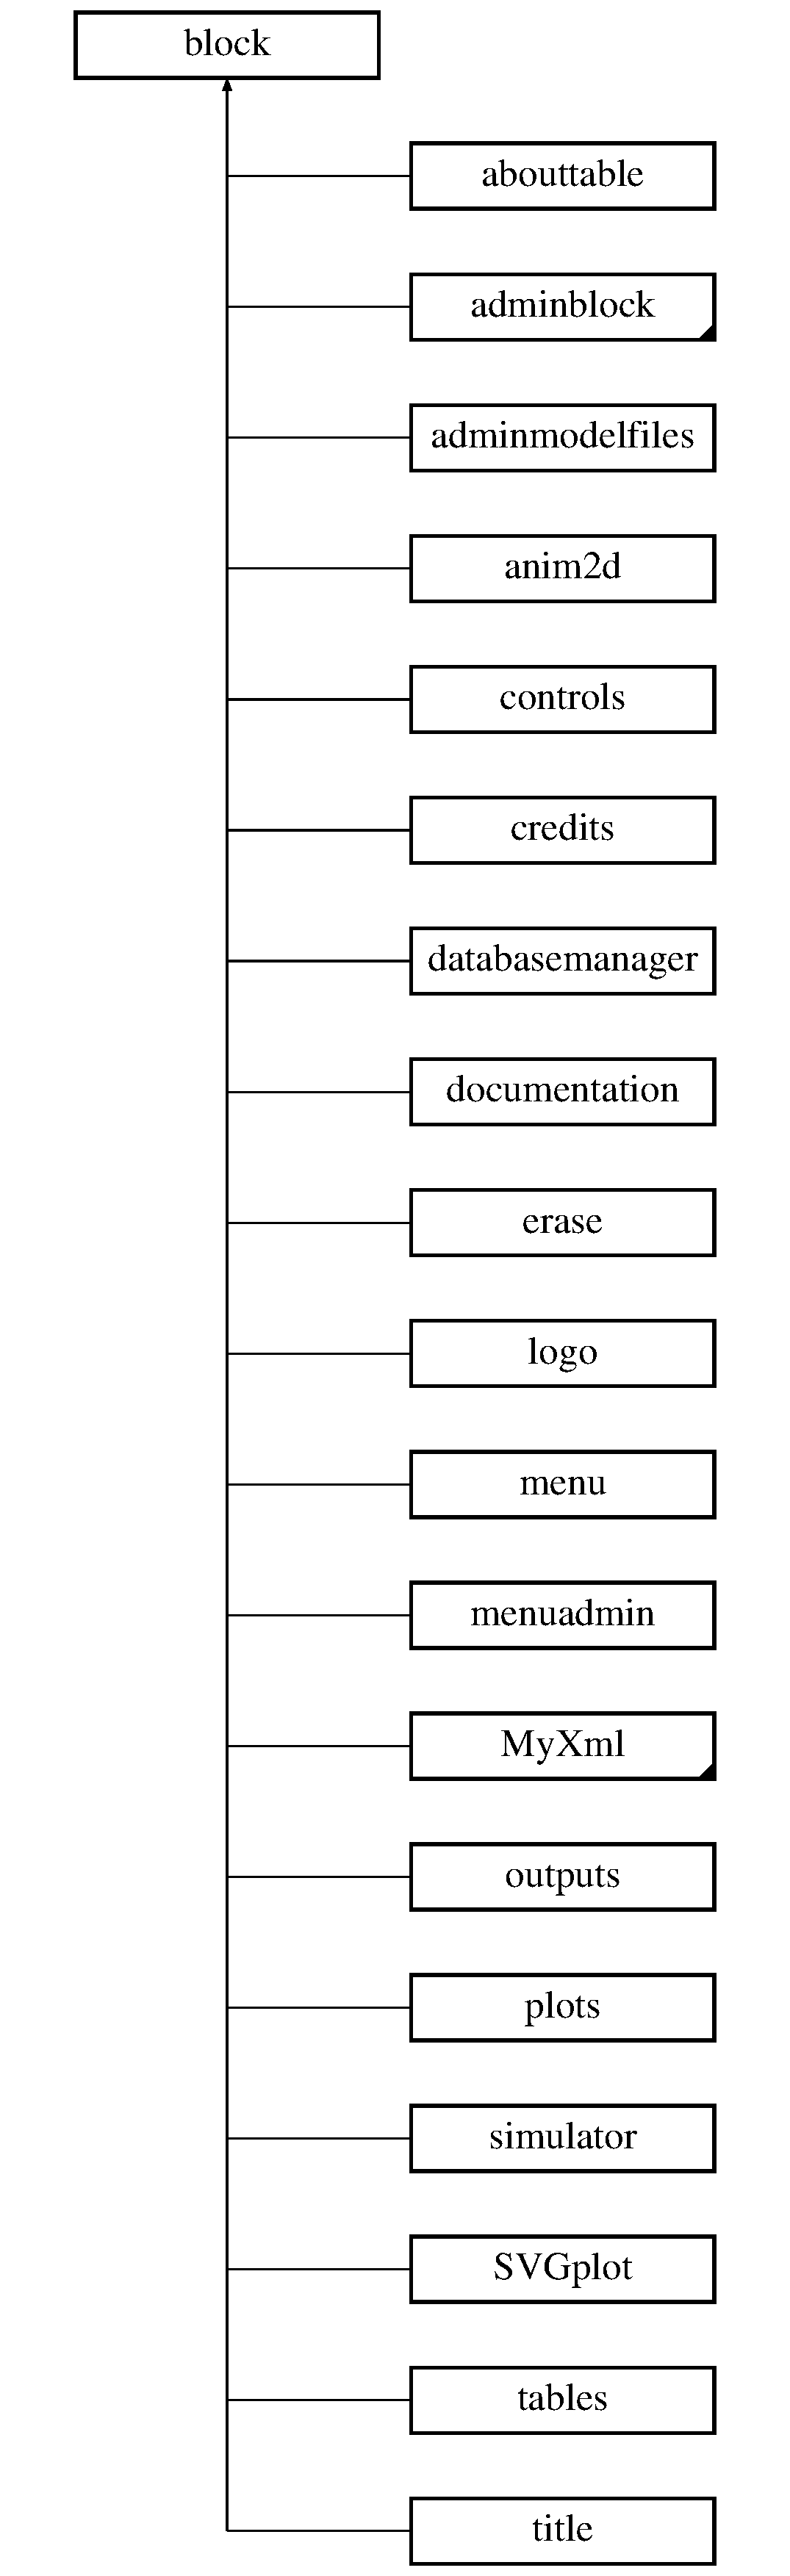
\includegraphics[height=12.000000cm]{classblock}
\end{center}
\end{figure}
\subsection*{\-Métodos públicos}
\begin{DoxyCompactItemize}
\item 
\hypertarget{classblock_a9b390283efee92f54e6eed6c281155ad}{{\bfseries block} ()}\label{classblock_a9b390283efee92f54e6eed6c281155ad}

\item 
\hypertarget{classblock_a975c7c9239a25602f4b457fdc430762f}{{\bfseries connect} ()}\label{classblock_a975c7c9239a25602f4b457fdc430762f}

\item 
\hypertarget{classblock_a079f285ef5aaeee792021a3850426879}{{\bfseries text} (\$str)}\label{classblock_a079f285ef5aaeee792021a3850426879}

\item 
\hypertarget{classblock_a0f1cfe5eb0f56e9c1b2a37c2ed64cf4b}{{\bfseries validate\-Value} (\$type, \$par\-\_\-id, \$new\-\_\-value, \$default\-\_\-value)}\label{classblock_a0f1cfe5eb0f56e9c1b2a37c2ed64cf4b}

\item 
\hypertarget{classblock_a3b3442844224e1bf4f576867bbf541e9}{{\bfseries opener} ()}\label{classblock_a3b3442844224e1bf4f576867bbf541e9}

\item 
\hypertarget{classblock_ae721cd25adbb868cb7184ccdd71c919a}{{\bfseries closer} ()}\label{classblock_ae721cd25adbb868cb7184ccdd71c919a}

\item 
\hypertarget{classblock_a40a4d88a8dd0bace93b171030a3f5379}{{\bfseries html\-Simple\-Open} (\$\-Xml, \$nivel)}\label{classblock_a40a4d88a8dd0bace93b171030a3f5379}

\item 
\hypertarget{classblock_ade8c7b59b5d23272ee5356cf804ed6fa}{{\bfseries html\-Simple\-Close} (\$\-Xml, \$nivel)}\label{classblock_ade8c7b59b5d23272ee5356cf804ed6fa}

\item 
\hypertarget{classblock_a4b7ba71e210f75b44e7f86d5948cb1af}{{\bfseries html\-Block} (\$\-Xml, \$nivel)}\label{classblock_a4b7ba71e210f75b44e7f86d5948cb1af}

\item 
\hypertarget{classblock_a97726852fcd6a5a1383fed3294abd491}{{\bfseries html} (\$xml\-F\-N)}\label{classblock_a97726852fcd6a5a1383fed3294abd491}

\item 
\hypertarget{classblock_a5759868815bd72fdd3661f9da08d1417}{{\bfseries read\-Xml} (\$fn)}\label{classblock_a5759868815bd72fdd3661f9da08d1417}

\item 
\hypertarget{classblock_aee88fc7c18e29468d15803b44020eda3}{{\bfseries enabled} (\$table)}\label{classblock_aee88fc7c18e29468d15803b44020eda3}

\item 
\hypertarget{classblock_ac64202719db0181f3f7ae8d0b200748d}{{\bfseries x\-\_\-id} (\$key)}\label{classblock_ac64202719db0181f3f7ae8d0b200748d}

\item 
\hypertarget{classblock_a1cc5bea23727f931100aae223be6fb50}{{\bfseries modeller\-\_\-id} ()}\label{classblock_a1cc5bea23727f931100aae223be6fb50}

\item 
\hypertarget{classblock_a435a58035b2fd36de73e20a62afb119d}{{\bfseries c2deffect\-\_\-id} ()}\label{classblock_a435a58035b2fd36de73e20a62afb119d}

\item 
\hypertarget{classblock_ae28a0750c95c5a9c8d32257c7e8e4cb3}{{\bfseries c2danimation\-\_\-id} ()}\label{classblock_ae28a0750c95c5a9c8d32257c7e8e4cb3}

\item 
\hypertarget{classblock_ad2e5d2a9c0f265168608d809e8434769}{{\bfseries control\-\_\-id} ()}\label{classblock_ad2e5d2a9c0f265168608d809e8434769}

\item 
\hypertarget{classblock_abb00b6e42531fc704f1e4cc73d4ff55b}{{\bfseries practice\-\_\-id} ()}\label{classblock_abb00b6e42531fc704f1e4cc73d4ff55b}

\item 
\hypertarget{classblock_a055d9a000b949c39e4f235d2d95df209}{{\bfseries control\-\_\-group\-\_\-id} ()}\label{classblock_a055d9a000b949c39e4f235d2d95df209}

\item 
\hypertarget{classblock_af5ed792d253caab1dc6c87bbdb812103}{{\bfseries curve\-\_\-id} ()}\label{classblock_af5ed792d253caab1dc6c87bbdb812103}

\item 
\hypertarget{classblock_aa28baa9be3ba32284dbb684b2a7dad25}{{\bfseries plot\-\_\-id} ()}\label{classblock_aa28baa9be3ba32284dbb684b2a7dad25}

\item 
\hypertarget{classblock_a11c3a1c6c6ab19d00a291d6dedcadcfb}{{\bfseries model\-\_\-id} ()}\label{classblock_a11c3a1c6c6ab19d00a291d6dedcadcfb}

\item 
\hypertarget{classblock_a5b4e278984fb6f58474ba1318e473655}{{\bfseries section\-\_\-id} ()}\label{classblock_a5b4e278984fb6f58474ba1318e473655}

\item 
\hypertarget{classblock_afff17cca8d1e2ec77ae40b6867eaa7fe}{{\bfseries display} ()}\label{classblock_afff17cca8d1e2ec77ae40b6867eaa7fe}

\end{DoxyCompactItemize}
\subsection*{\-Atributos públicos}
\begin{DoxyCompactItemize}
\item 
\hypertarget{classblock_a1c94cbb3bc0af9407e08d5bf372c1a45}{{\bfseries \$\-Xml}}\label{classblock_a1c94cbb3bc0af9407e08d5bf372c1a45}

\item 
\hypertarget{classblock_a253606399d635e084dee7745be77f925}{{\bfseries \$strings}}\label{classblock_a253606399d635e084dee7745be77f925}

\item 
\hypertarget{classblock_a7793d302164a793a4b94620e90f019f1}{{\bfseries \$configuration\-Settings}}\label{classblock_a7793d302164a793a4b94620e90f019f1}

\end{DoxyCompactItemize}


\subsection{\-Descripción detallada}


\-Definición en la línea 5 del archivo block.\-php.



\-La documentación para esta clase fue generada a partir del siguiente fichero\-:\begin{DoxyCompactItemize}
\item 
block.\-php\end{DoxyCompactItemize}

\hypertarget{classconfiguration}{\section{\-Referencia de la \-Clase configuration}
\label{classconfiguration}\index{configuration@{configuration}}
}
\subsection*{\-Métodos públicos}
\begin{DoxyCompactItemize}
\item 
\hypertarget{classconfiguration_a67baa5b1b19e6ab5b7d99d3704804f30}{{\bfseries readconfig} (\$configfile)}\label{classconfiguration_a67baa5b1b19e6ab5b7d99d3704804f30}

\item 
\hypertarget{classconfiguration_ac2a22ec1c4e26f015276561876d2e48f}{{\bfseries writeconfig} (\$configfile, \$changes)}\label{classconfiguration_ac2a22ec1c4e26f015276561876d2e48f}

\end{DoxyCompactItemize}


\subsection{\-Descripción detallada}


\-Definición en la línea 2 del archivo config.\-class.\-php.



\-La documentación para esta clase fue generada a partir del siguiente fichero\-:\begin{DoxyCompactItemize}
\item 
config/config.\-class.\-php\end{DoxyCompactItemize}

\hypertarget{classcontrols}{}\section{Referencia de la Clase controls}
\label{classcontrols}\index{controls@{controls}}
Diagrama de herencias de controls\begin{figure}[H]
\begin{center}
\leavevmode
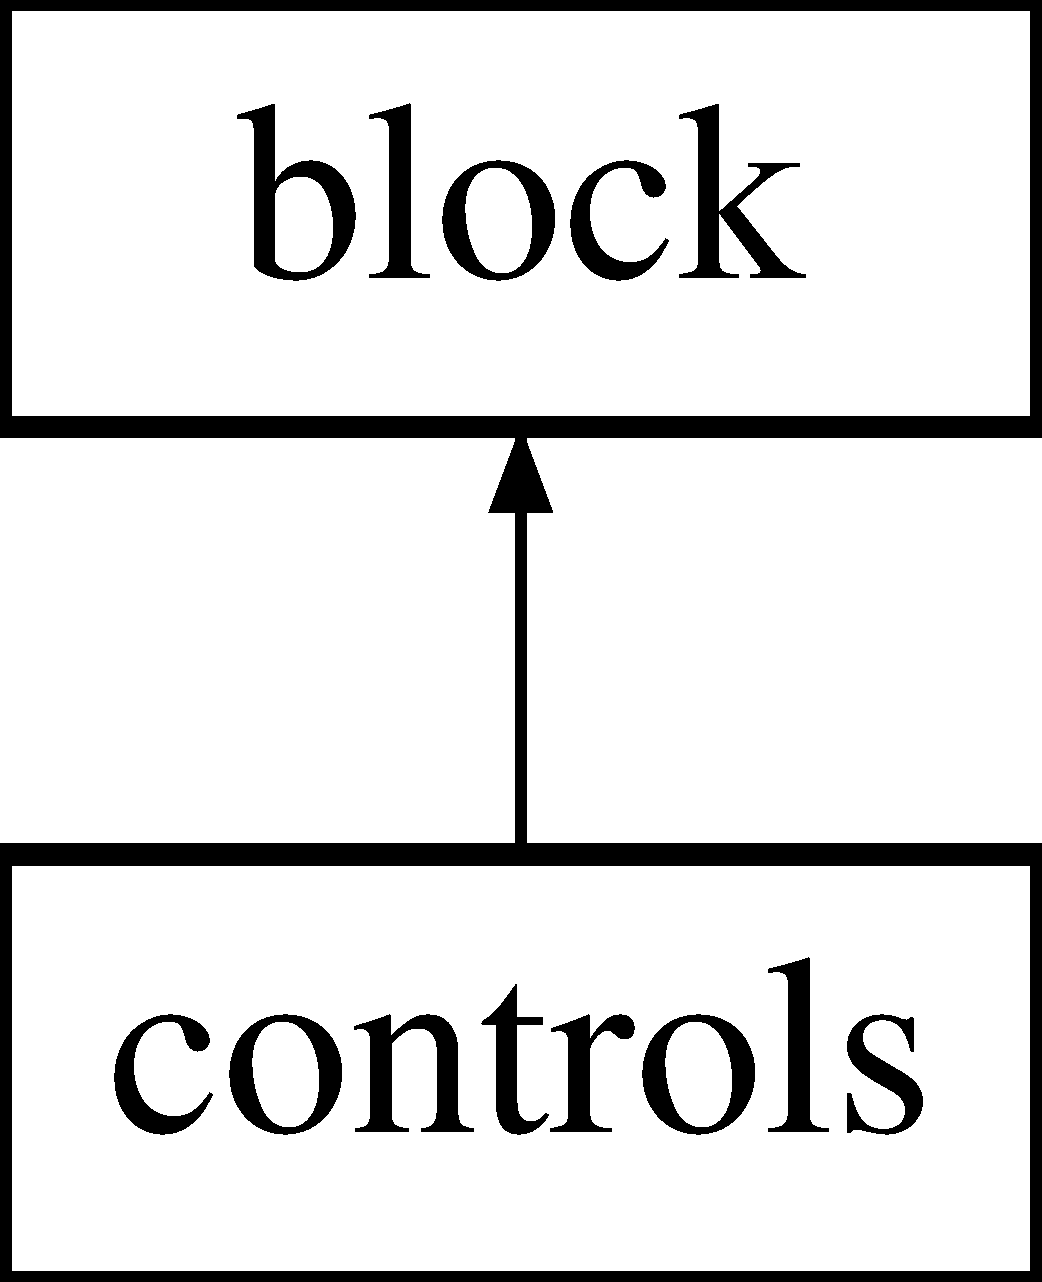
\includegraphics[height=2.000000cm]{classcontrols}
\end{center}
\end{figure}
\subsection*{Métodos públicos}
\begin{DoxyCompactItemize}
\item 
\mbox{\Hypertarget{classcontrols_a04cc5e8f1b02044b282605cc3ec3618b}\label{classcontrols_a04cc5e8f1b02044b282605cc3ec3618b}} 
{\bfseries display\+Control} (\$data)
\item 
\mbox{\Hypertarget{classcontrols_a8f5e4c575408639040ae2ed3b0e5d48d}\label{classcontrols_a8f5e4c575408639040ae2ed3b0e5d48d}} 
{\bfseries display\+Select} (\$data)
\item 
\mbox{\Hypertarget{classcontrols_abeb2846c5ecd32ab5bfcb2769564854d}\label{classcontrols_abeb2846c5ecd32ab5bfcb2769564854d}} 
{\bfseries display\+Controls} (\$control\+\_\+group\+\_\+id)
\item 
\mbox{\Hypertarget{classcontrols_aa7b6356102da29a6789c8d22b0f41d40}\label{classcontrols_aa7b6356102da29a6789c8d22b0f41d40}} 
{\bfseries datos} (\$model\+\_\+id)
\item 
\mbox{\Hypertarget{classcontrols_adcf32ff72657c72dbcb1416b62f2c30b}\label{classcontrols_adcf32ff72657c72dbcb1416b62f2c30b}} 
{\bfseries javascript} ()
\item 
\mbox{\Hypertarget{classcontrols_a96d2e836bcf5c210d1231f289917f037}\label{classcontrols_a96d2e836bcf5c210d1231f289917f037}} 
{\bfseries ecmascript} ()
\item 
\mbox{\Hypertarget{classcontrols_a0dc99645804c3ffe83de9d175b5ccfb1}\label{classcontrols_a0dc99645804c3ffe83de9d175b5ccfb1}} 
{\bfseries display} ()
\end{DoxyCompactItemize}
\subsection*{Atributos públicos}
\begin{DoxyCompactItemize}
\item 
\mbox{\Hypertarget{classcontrols_abda28107af4943a229e1346924684183}\label{classcontrols_abda28107af4943a229e1346924684183}} 
{\bfseries \$datos}
\end{DoxyCompactItemize}


\subsection{Descripción detallada}


Definición en la línea 4 del archivo controls.\+php.



La documentación para esta clase fue generada a partir del siguiente fichero\+:\begin{DoxyCompactItemize}
\item 
/home/ogduartev/public\+\_\+html/unvl-\/\+Git\+Hub/\+U\+N\+Virtual\+Lab/controls.\+php\end{DoxyCompactItemize}

\hypertarget{classcredits}{}\section{Referencia de la Clase credits}
\label{classcredits}\index{credits@{credits}}
Diagrama de herencias de credits\begin{figure}[H]
\begin{center}
\leavevmode
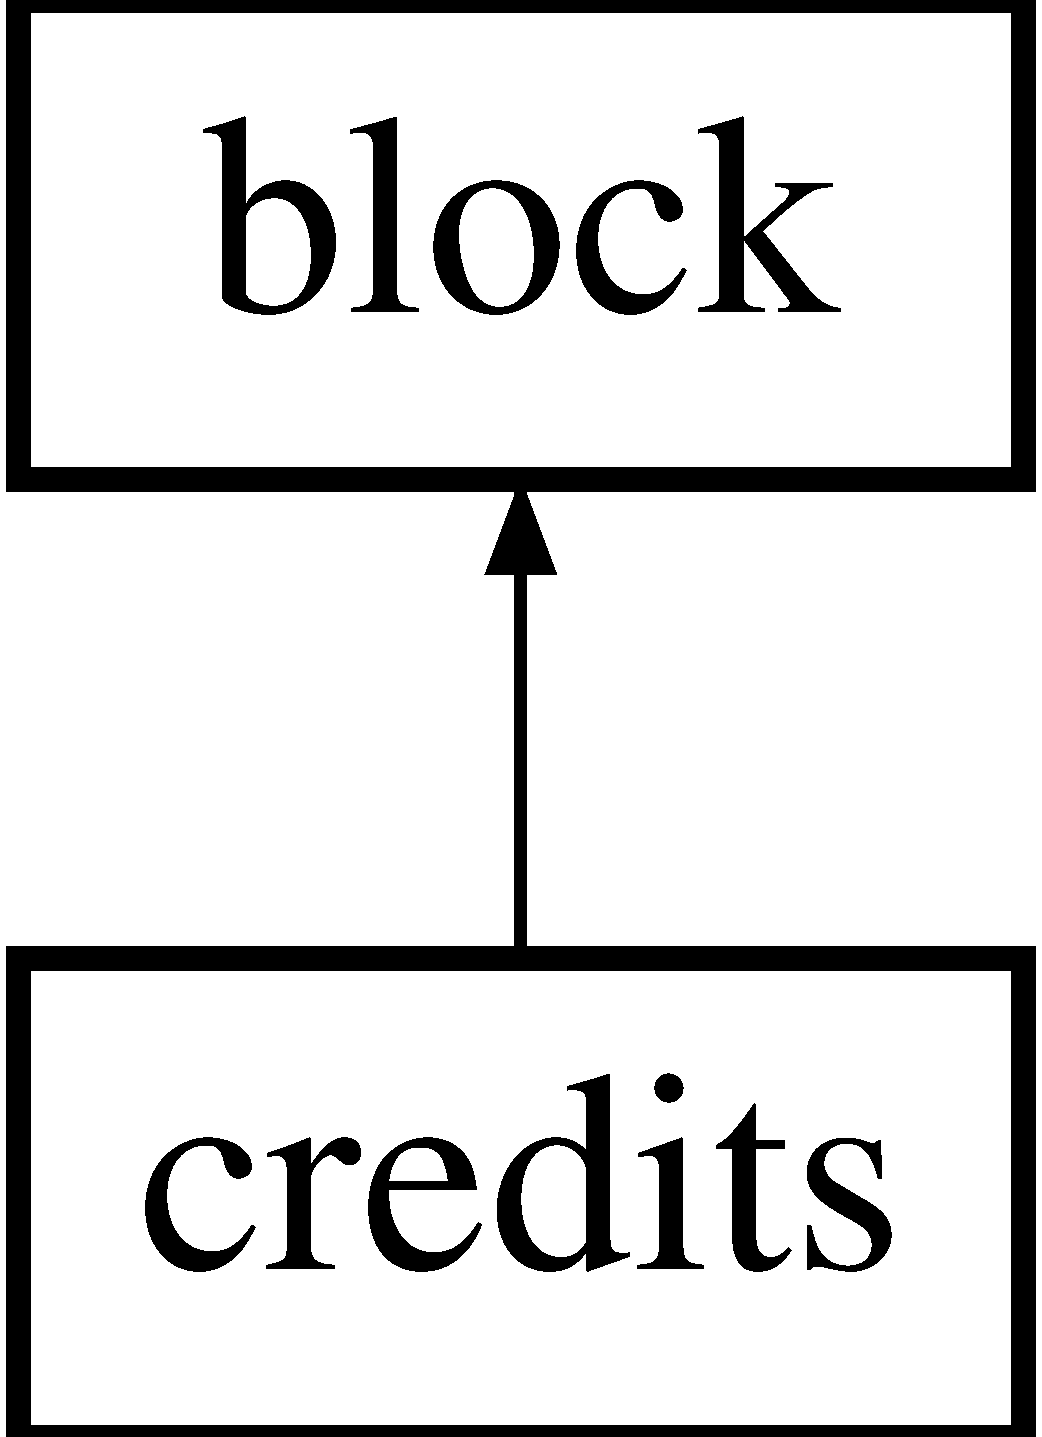
\includegraphics[height=2.000000cm]{classcredits}
\end{center}
\end{figure}
\subsection*{Métodos públicos}
\begin{DoxyCompactItemize}
\item 
\mbox{\Hypertarget{classcredits_aed4f2bfc57e15cd9e2749ff7411a9be6}\label{classcredits_aed4f2bfc57e15cd9e2749ff7411a9be6}} 
{\bfseries display} ()
\end{DoxyCompactItemize}
\subsection*{Otros miembros heredados}


\subsection{Descripción detallada}


Definición en la línea 4 del archivo credits.\+php.



La documentación para esta clase fue generada a partir del siguiente fichero\+:\begin{DoxyCompactItemize}
\item 
/home/ogduartev/public\+\_\+html/unvl-\/\+Git\+Hub/\+U\+N\+Virtual\+Lab/credits.\+php\end{DoxyCompactItemize}

\hypertarget{classcsvreader}{\section{\-Referencia de la \-Clase csvreader}
\label{classcsvreader}\index{csvreader@{csvreader}}
}
\subsection*{\-Métodos públicos}
\begin{DoxyCompactItemize}
\item 
\hypertarget{classcsvreader_aa452a501204476ec83163c625a75e709}{{\bfseries read\-Csv} (\$fn)}\label{classcsvreader_aa452a501204476ec83163c625a75e709}

\item 
\hypertarget{classcsvreader_a0dcd4aba99b7cfc585420b96bc3e8618}{{\bfseries read\-Sync} (\$fn)}\label{classcsvreader_a0dcd4aba99b7cfc585420b96bc3e8618}

\end{DoxyCompactItemize}


\subsection{\-Descripción detallada}


\-Definición en la línea 3 del archivo csvreader.\-php.



\-La documentación para esta clase fue generada a partir del siguiente fichero\-:\begin{DoxyCompactItemize}
\item 
csvreader.\-php\end{DoxyCompactItemize}

\hypertarget{classdatabasemanager}{\section{\-Referencia de la \-Clase databasemanager}
\label{classdatabasemanager}\index{databasemanager@{databasemanager}}
}
\-Diagrama de herencias de databasemanager\begin{figure}[H]
\begin{center}
\leavevmode
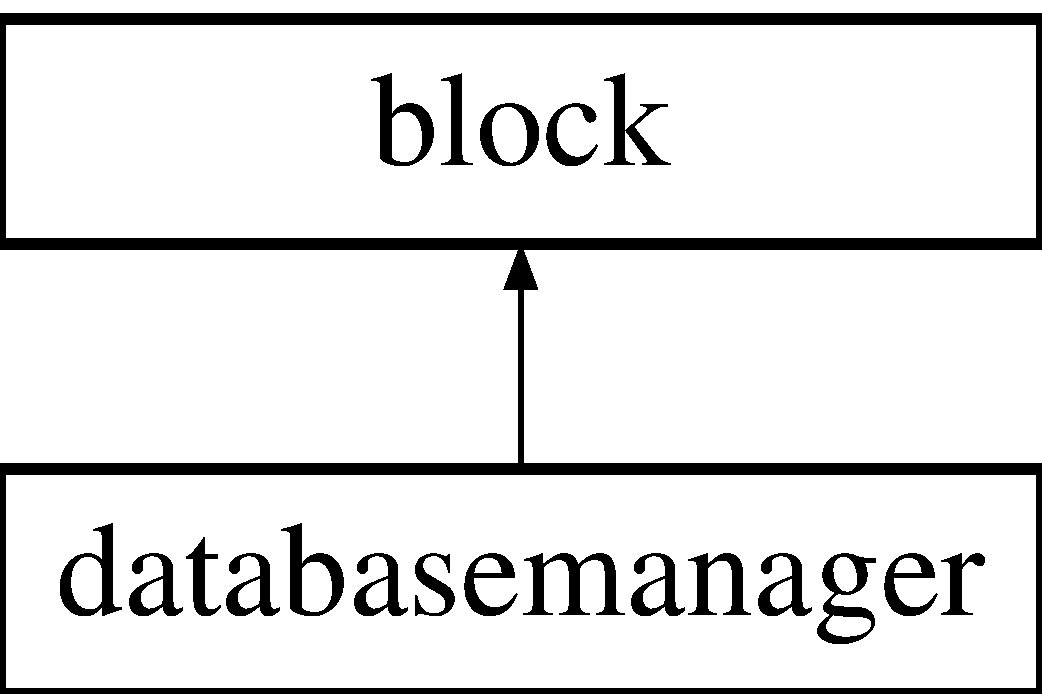
\includegraphics[height=2.000000cm]{classdatabasemanager}
\end{center}
\end{figure}
\subsection*{\-Métodos públicos}
\begin{DoxyCompactItemize}
\item 
\hypertarget{classdatabasemanager_a23e8b4bd50cb6cae2007eb148f5e99ab}{{\bfseries update} (\$table, \$idname, \$idvalue)}\label{classdatabasemanager_a23e8b4bd50cb6cae2007eb148f5e99ab}

\item 
\hypertarget{classdatabasemanager_adb5e50ea96be1714588592eb5024f0b3}{{\bfseries update1\-N\-N1} (\$idvalue)}\label{classdatabasemanager_adb5e50ea96be1714588592eb5024f0b3}

\item 
\hypertarget{classdatabasemanager_ac215ce5b47d2f5bfa36621fe45b3eedf}{{\bfseries insert} ()}\label{classdatabasemanager_ac215ce5b47d2f5bfa36621fe45b3eedf}

\item 
\hypertarget{classdatabasemanager_a09e06d8512461851688d5a34d5a31c1d}{{\bfseries insert1\-N\-N1} (\$idvalue)}\label{classdatabasemanager_a09e06d8512461851688d5a34d5a31c1d}

\item 
\hypertarget{classdatabasemanager_a86356dce647d0d5c74ff78276844f8ca}{{\bfseries delete} ()}\label{classdatabasemanager_a86356dce647d0d5c74ff78276844f8ca}

\item 
\hypertarget{classdatabasemanager_ac40bb924bbe6dff5aba9f0c1636a2fdd}{{\bfseries delete1\-N\-N1} (\$idvalue)}\label{classdatabasemanager_ac40bb924bbe6dff5aba9f0c1636a2fdd}

\item 
\hypertarget{classdatabasemanager_ad3462cf95718f57f3c7cc634c9d3a829}{{\bfseries create\-Directories} (\$id)}\label{classdatabasemanager_ad3462cf95718f57f3c7cc634c9d3a829}

\item 
\hypertarget{classdatabasemanager_a183c2e82b2a4d6429fea64565a723a47}{{\bfseries delete\-Dir} (\$dir)}\label{classdatabasemanager_a183c2e82b2a4d6429fea64565a723a47}

\item 
\hypertarget{classdatabasemanager_a4f77b12a19b44a980cf33c833ce27b21}{{\bfseries delete\-Directories} (\$id)}\label{classdatabasemanager_a4f77b12a19b44a980cf33c833ce27b21}

\item 
\hypertarget{classdatabasemanager_a321eb1187e03a72d03509388b3daddec}{{\bfseries display} ()}\label{classdatabasemanager_a321eb1187e03a72d03509388b3daddec}

\end{DoxyCompactItemize}


\subsection{\-Descripción detallada}


\-Definición en la línea 4 del archivo databasemanager.\-php.



\-La documentación para esta clase fue generada a partir del siguiente fichero\-:\begin{DoxyCompactItemize}
\item 
admin/databasemanager.\-php\end{DoxyCompactItemize}

\hypertarget{classdocumentation}{}\section{Referencia de la Clase documentation}
\label{classdocumentation}\index{documentation@{documentation}}
Diagrama de herencias de documentation\begin{figure}[H]
\begin{center}
\leavevmode
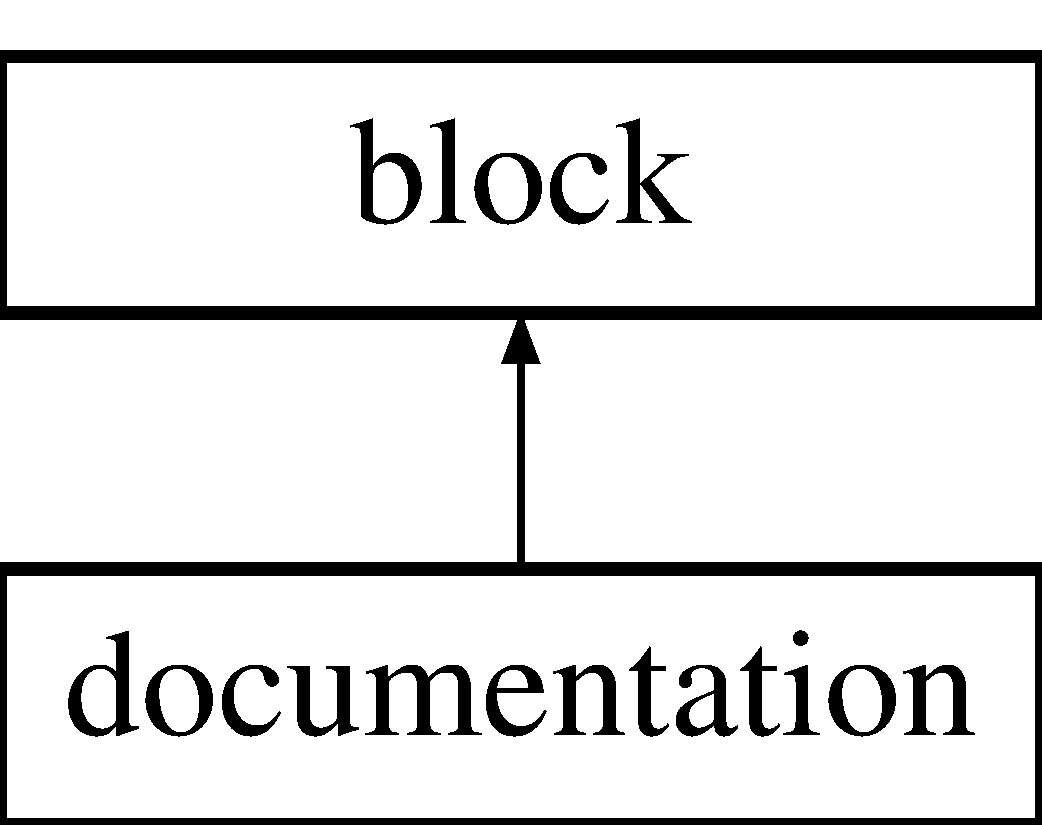
\includegraphics[height=2.000000cm]{classdocumentation}
\end{center}
\end{figure}
\subsection*{Métodos públicos}
\begin{DoxyCompactItemize}
\item 
\mbox{\Hypertarget{classdocumentation_a57d71d7b60444440fa1a4aba1135a751}\label{classdocumentation_a57d71d7b60444440fa1a4aba1135a751}} 
{\bfseries display} ()
\item 
\mbox{\Hypertarget{classdocumentation_ad83e35dbf443ee7ee2b6efafcc7f36a6}\label{classdocumentation_ad83e35dbf443ee7ee2b6efafcc7f36a6}} 
{\bfseries display\+Message} ()
\end{DoxyCompactItemize}
\subsection*{Otros miembros heredados}


\subsection{Descripción detallada}


Definición en la línea 4 del archivo documentation.\+php.



La documentación para esta clase fue generada a partir del siguiente fichero\+:\begin{DoxyCompactItemize}
\item 
/home/ogduartev/public\+\_\+html/unvl-\/\+Git\+Hub/\+U\+N\+Virtual\+Lab/documentation.\+php\end{DoxyCompactItemize}

\hypertarget{classerase}{\section{\-Referencia de la \-Clase erase}
\label{classerase}\index{erase@{erase}}
}
\-Diagrama de herencias de erase\begin{figure}[H]
\begin{center}
\leavevmode
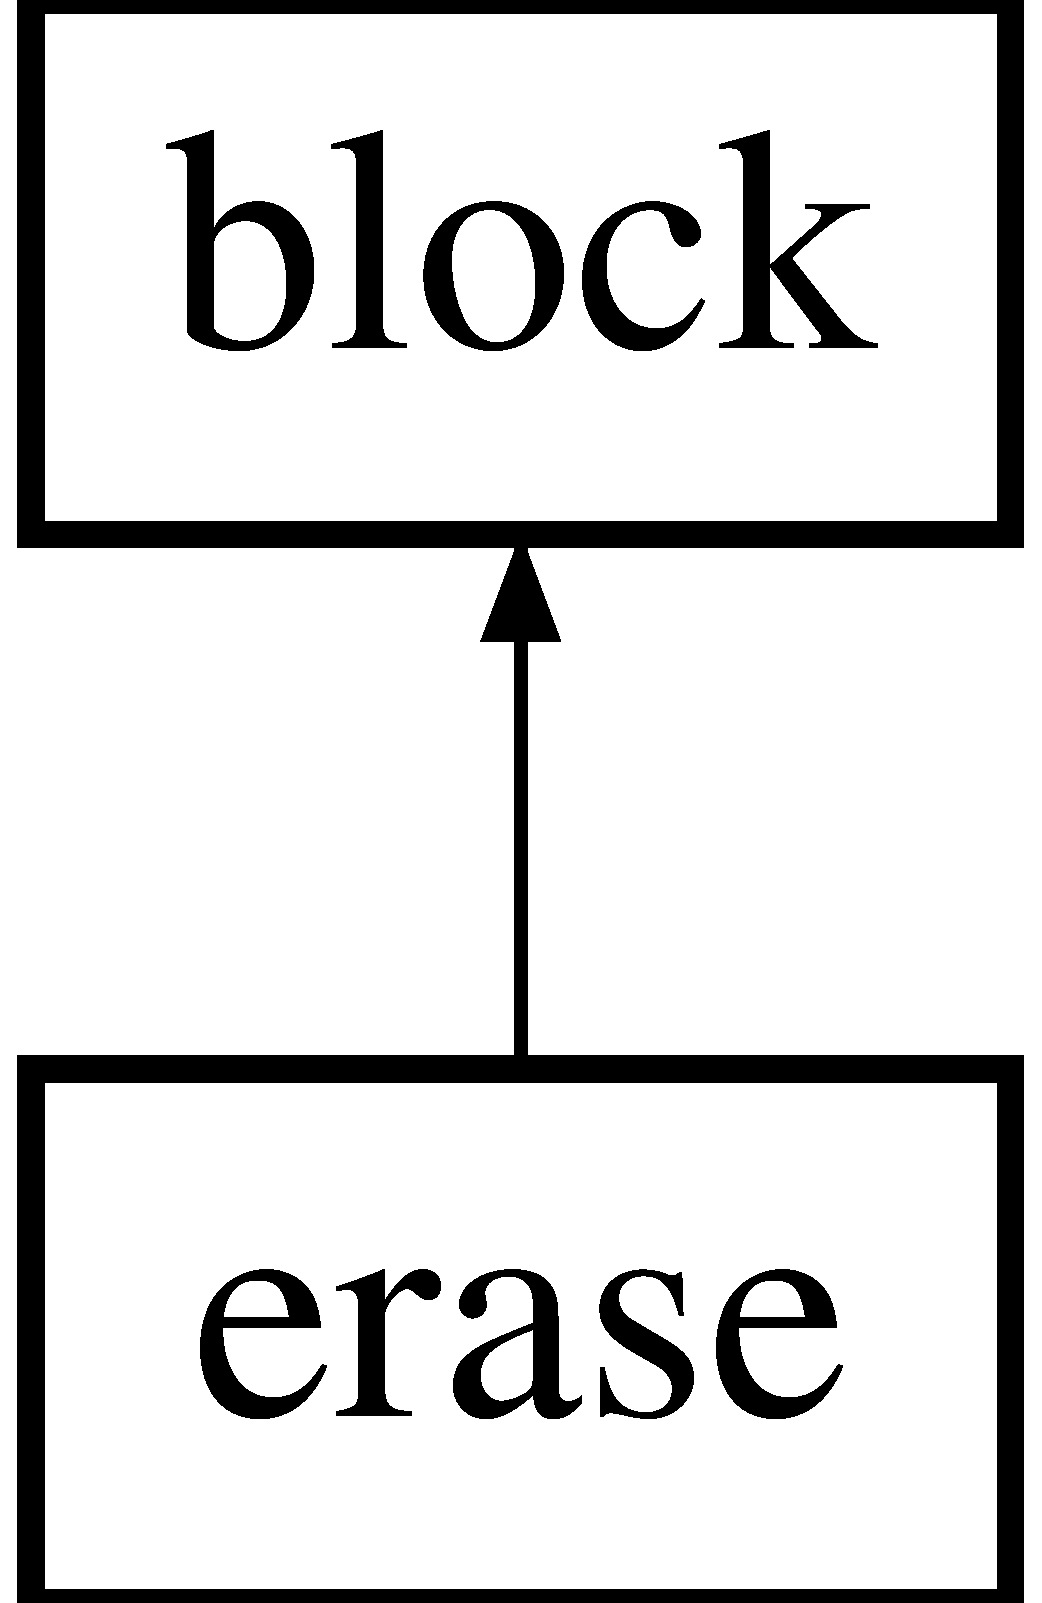
\includegraphics[height=2.000000cm]{classerase}
\end{center}
\end{figure}
\subsection*{\-Métodos públicos}
\begin{DoxyCompactItemize}
\item 
\hypertarget{classerase_a1d79faabec523c39a5662d10682acec8}{{\bfseries display} ()}\label{classerase_a1d79faabec523c39a5662d10682acec8}

\end{DoxyCompactItemize}


\subsection{\-Descripción detallada}


\-Definición en la línea 4 del archivo erase.\-php.



\-La documentación para esta clase fue generada a partir del siguiente fichero\-:\begin{DoxyCompactItemize}
\item 
erase.\-php\end{DoxyCompactItemize}

\hypertarget{classexport}{\section{\-Referencia de la \-Clase export}
\label{classexport}\index{export@{export}}
}
\subsection*{\-Métodos públicos}
\begin{DoxyCompactItemize}
\item 
\hypertarget{classexport_a6bb9adef631ba2c4e6c145c9e8f65d0e}{{\bfseries export} ()}\label{classexport_a6bb9adef631ba2c4e6c145c9e8f65d0e}

\item 
\hypertarget{classexport_a7491b9998567bd762e24f5c9be0e9a38}{{\bfseries connect} ()}\label{classexport_a7491b9998567bd762e24f5c9be0e9a38}

\item 
\hypertarget{classexport_a21bab30d532758a7a55156a4f06cb266}{{\bfseries export\-Line} (\$table, \$line)}\label{classexport_a21bab30d532758a7a55156a4f06cb266}

\item 
\hypertarget{classexport_abbd1e1328e3da9f01b20e506935722d6}{{\bfseries export\-Modellers\-Models} (\$id)}\label{classexport_abbd1e1328e3da9f01b20e506935722d6}

\item 
\hypertarget{classexport_a582ace8f99822af23299fcd2209295c9}{{\bfseries export\-Table\-Array} (\$tn, \$idn, \$id)}\label{classexport_a582ace8f99822af23299fcd2209295c9}

\item 
\hypertarget{classexport_a90fe702f9b0a74dc81c9d0986c2b23fc}{{\bfseries export\-Table} (\$tn, \$idn, \$id)}\label{classexport_a90fe702f9b0a74dc81c9d0986c2b23fc}

\item 
\hypertarget{classexport_a50fa4458dbe94ed2c6ea9e4a616728cd}{{\bfseries export\-Table2} (\$tn, \$idn, \$mid)}\label{classexport_a50fa4458dbe94ed2c6ea9e4a616728cd}

\item 
\hypertarget{classexport_a6f0205af2076d84df46cc761ec1c068b}{{\bfseries export\-Tables} (\$model\-I\-D)}\label{classexport_a6f0205af2076d84df46cc761ec1c068b}

\item 
\hypertarget{classexport_abdd608d3ef87829b0e3750fad13b10f2}{{\bfseries export\-Str} ()}\label{classexport_abdd608d3ef87829b0e3750fad13b10f2}

\end{DoxyCompactItemize}
\subsection*{\-Atributos públicos}
\begin{DoxyCompactItemize}
\item 
\hypertarget{classexport_ad82d75c031cf67d8890ffc9c9695948d}{{\bfseries \$tables}}\label{classexport_ad82d75c031cf67d8890ffc9c9695948d}

\item 
\hypertarget{classexport_a78444bac26d987c08fcdc31ef7b0088f}{{\bfseries \$configuration\-Settings}}\label{classexport_a78444bac26d987c08fcdc31ef7b0088f}

\end{DoxyCompactItemize}


\subsection{\-Descripción detallada}


\-Definición en la línea 4 del archivo export\-Model.\-php.



\-La documentación para esta clase fue generada a partir del siguiente fichero\-:\begin{DoxyCompactItemize}
\item 
samples/export\-Model.\-php\end{DoxyCompactItemize}

\hypertarget{classimport}{}\section{Referencia de la Clase import}
\label{classimport}\index{import@{import}}
\subsection*{Métodos públicos}
\begin{DoxyCompactItemize}
\item 
\mbox{\Hypertarget{classimport_a2c5438f4bf08ebd69e0675cb56f8f04e}\label{classimport_a2c5438f4bf08ebd69e0675cb56f8f04e}} 
{\bfseries import} ()
\item 
\mbox{\Hypertarget{classimport_a981c9e22a3d8c43548a62af334841e4a}\label{classimport_a981c9e22a3d8c43548a62af334841e4a}} 
{\bfseries connect} ()
\item 
\mbox{\Hypertarget{classimport_ae689e36a8b4bc859a2bdf953af65d9a4}\label{classimport_ae689e36a8b4bc859a2bdf953af65d9a4}} 
{\bfseries import\+Table} (\$tn, \$eqs)
\item 
\mbox{\Hypertarget{classimport_a79aec3c65f5939766d8bdf59de9037c7}\label{classimport_a79aec3c65f5939766d8bdf59de9037c7}} 
{\bfseries find\+Root\+Section} ()
\item 
\mbox{\Hypertarget{classimport_a4120da704a0f2ba63380c86bf5da00da}\label{classimport_a4120da704a0f2ba63380c86bf5da00da}} 
{\bfseries create\+Dirs} (\$id)
\item 
\mbox{\Hypertarget{classimport_abf37e24a7103afa8b9aa3e2ebde97d37}\label{classimport_abf37e24a7103afa8b9aa3e2ebde97d37}} 
{\bfseries import\+Tables} ()
\item 
\mbox{\Hypertarget{classimport_aee27bb889c83b03228c6c4337cdcf5de}\label{classimport_aee27bb889c83b03228c6c4337cdcf5de}} 
{\bfseries import\+Str} (\$fn)
\end{DoxyCompactItemize}
\subsection*{Atributos públicos}
\begin{DoxyCompactItemize}
\item 
\mbox{\Hypertarget{classimport_a44e9f11d7a5e167bd09b09d8fe090b1e}\label{classimport_a44e9f11d7a5e167bd09b09d8fe090b1e}} 
{\bfseries \$tables}
\item 
\mbox{\Hypertarget{classimport_a508b999d03da21afcbbe2f4a0f28a292}\label{classimport_a508b999d03da21afcbbe2f4a0f28a292}} 
{\bfseries \$id\+\_\+eq}
\item 
\mbox{\Hypertarget{classimport_a23438816c4c0d0e6aa3cd83f6224c8f1}\label{classimport_a23438816c4c0d0e6aa3cd83f6224c8f1}} 
{\bfseries \$configuration\+Settings}
\item 
\mbox{\Hypertarget{classimport_aa35f12e2cf3b02dac15d9c5f95902584}\label{classimport_aa35f12e2cf3b02dac15d9c5f95902584}} 
{\bfseries \$link}
\end{DoxyCompactItemize}


\subsection{Descripción detallada}


Definición en la línea 4 del archivo import\+Model.\+php.



La documentación para esta clase fue generada a partir del siguiente fichero\+:\begin{DoxyCompactItemize}
\item 
/home/ogduartev/public\+\_\+html/unvl-\/\+Git\+Hub/\+U\+N\+Virtual\+Lab/samples/import\+Model.\+php\end{DoxyCompactItemize}

\hypertarget{classlaunch}{}\section{Referencia de la Clase launch}
\label{classlaunch}\index{launch@{launch}}
Diagrama de herencias de launch\begin{figure}[H]
\begin{center}
\leavevmode
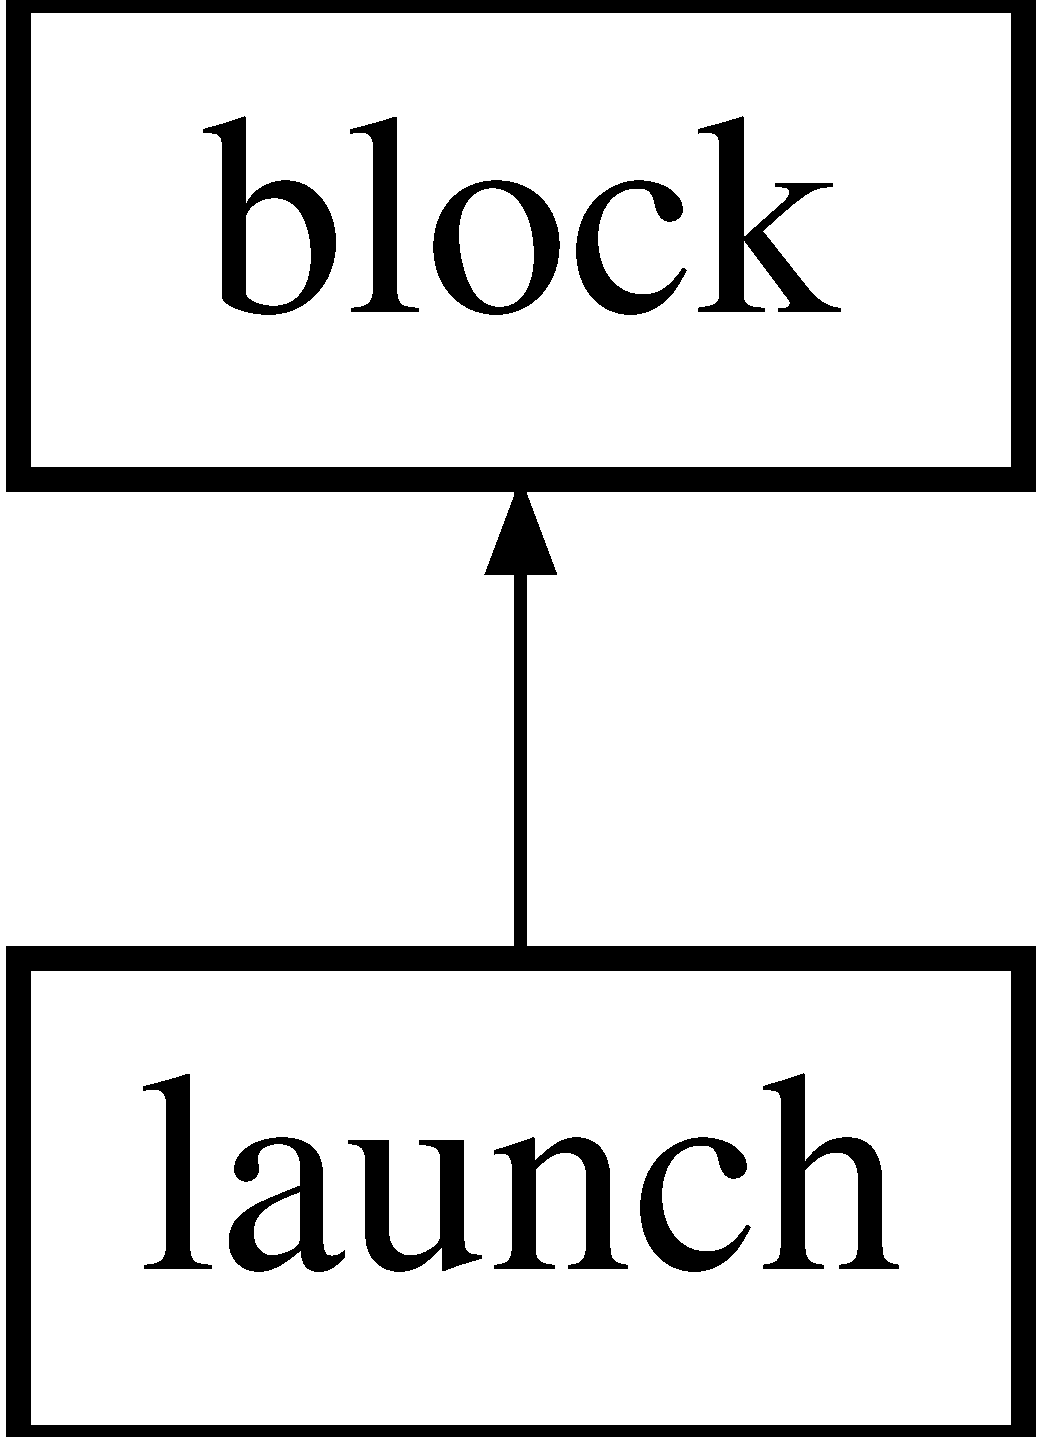
\includegraphics[height=2.000000cm]{classlaunch}
\end{center}
\end{figure}
\subsection*{Métodos públicos}
\begin{DoxyCompactItemize}
\item 
\mbox{\Hypertarget{classlaunch_adbcff964560eebe408b060ff667ff24b}\label{classlaunch_adbcff964560eebe408b060ff667ff24b}} 
{\bfseries display} ()
\end{DoxyCompactItemize}
\subsection*{Otros miembros heredados}


\subsection{Descripción detallada}


Definición en la línea 4 del archivo launch.\+php.



La documentación para esta clase fue generada a partir del siguiente fichero\+:\begin{DoxyCompactItemize}
\item 
/home/ogduartev/public\+\_\+html/unvl-\/\+Git\+Hub/\+U\+N\+Virtual\+Lab/launch.\+php\end{DoxyCompactItemize}

\hypertarget{classlogo}{\section{\-Referencia de la \-Clase logo}
\label{classlogo}\index{logo@{logo}}
}
\-Diagrama de herencias de logo\begin{figure}[H]
\begin{center}
\leavevmode
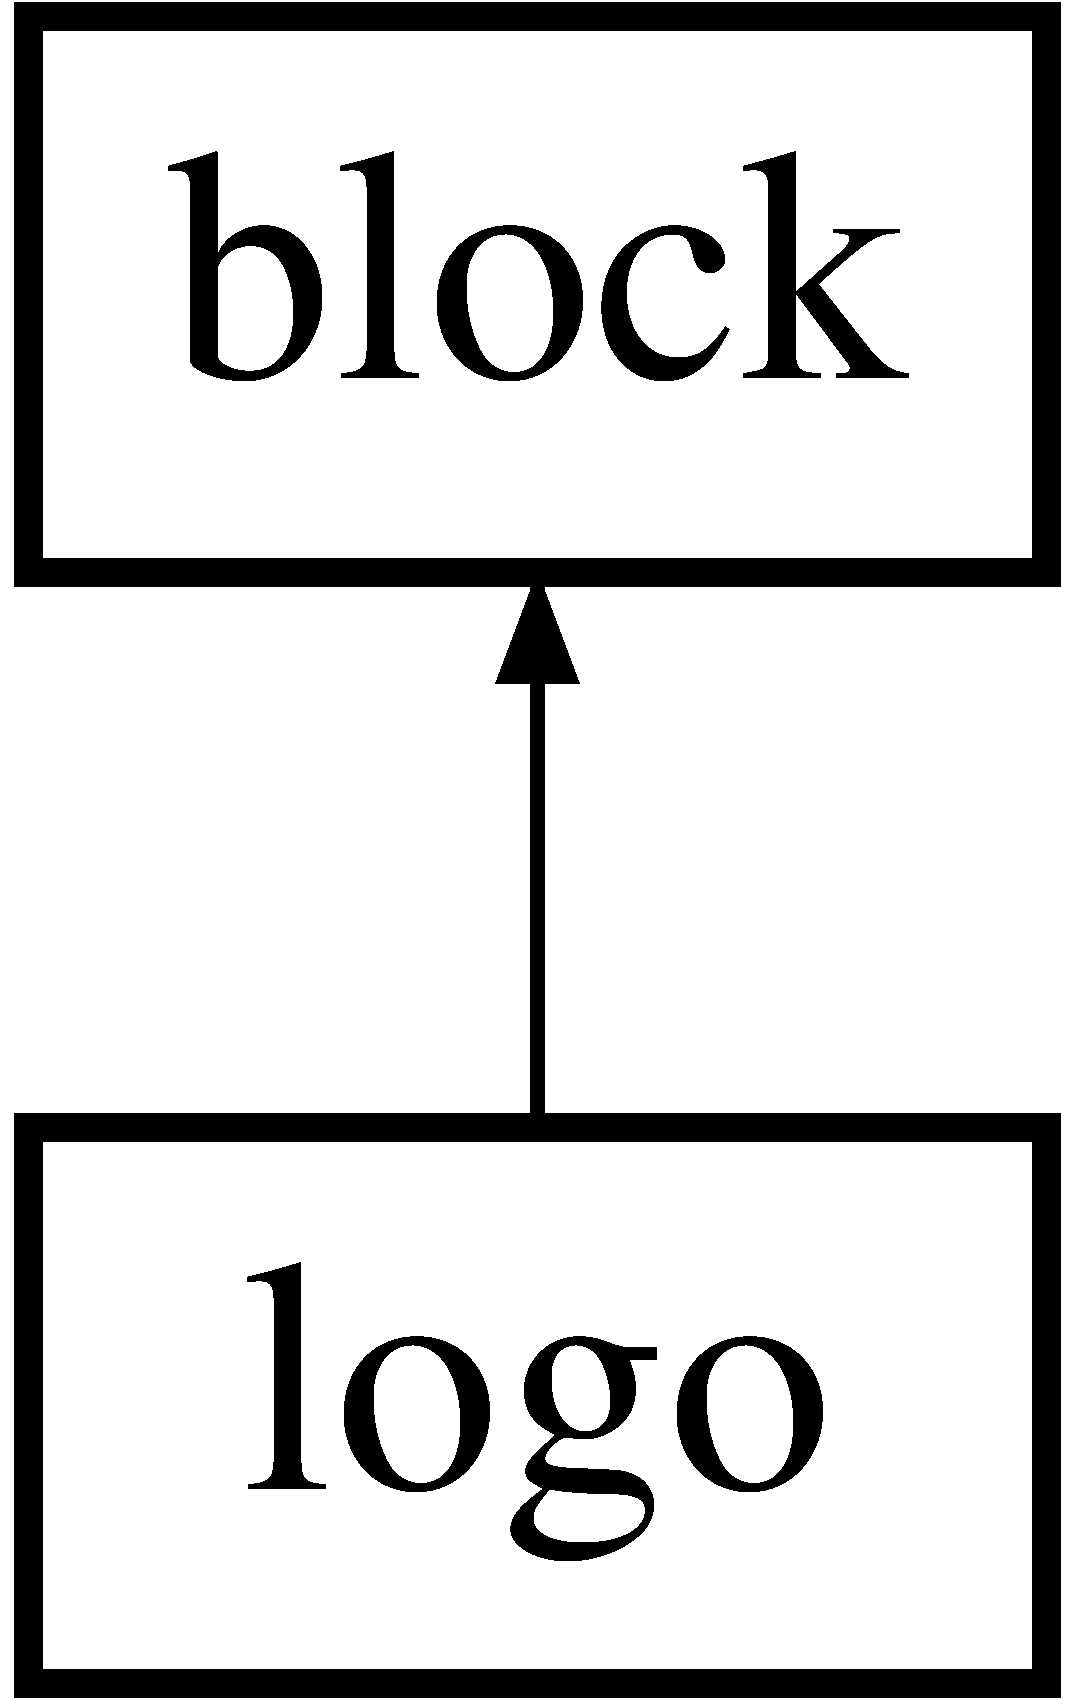
\includegraphics[height=2.000000cm]{classlogo}
\end{center}
\end{figure}
\subsection*{\-Métodos públicos}
\begin{DoxyCompactItemize}
\item 
\hypertarget{classlogo_a5dbc2e33bf0508b4ce4833f2799c1b99}{{\bfseries display} ()}\label{classlogo_a5dbc2e33bf0508b4ce4833f2799c1b99}

\end{DoxyCompactItemize}


\subsection{\-Descripción detallada}


\-Definición en la línea 4 del archivo logo.\-php.



\-La documentación para esta clase fue generada a partir del siguiente fichero\-:\begin{DoxyCompactItemize}
\item 
logo.\-php\end{DoxyCompactItemize}

\hypertarget{classmenu}{\section{\-Referencia de la \-Clase menu}
\label{classmenu}\index{menu@{menu}}
}
\-Diagrama de herencias de menu\begin{figure}[H]
\begin{center}
\leavevmode
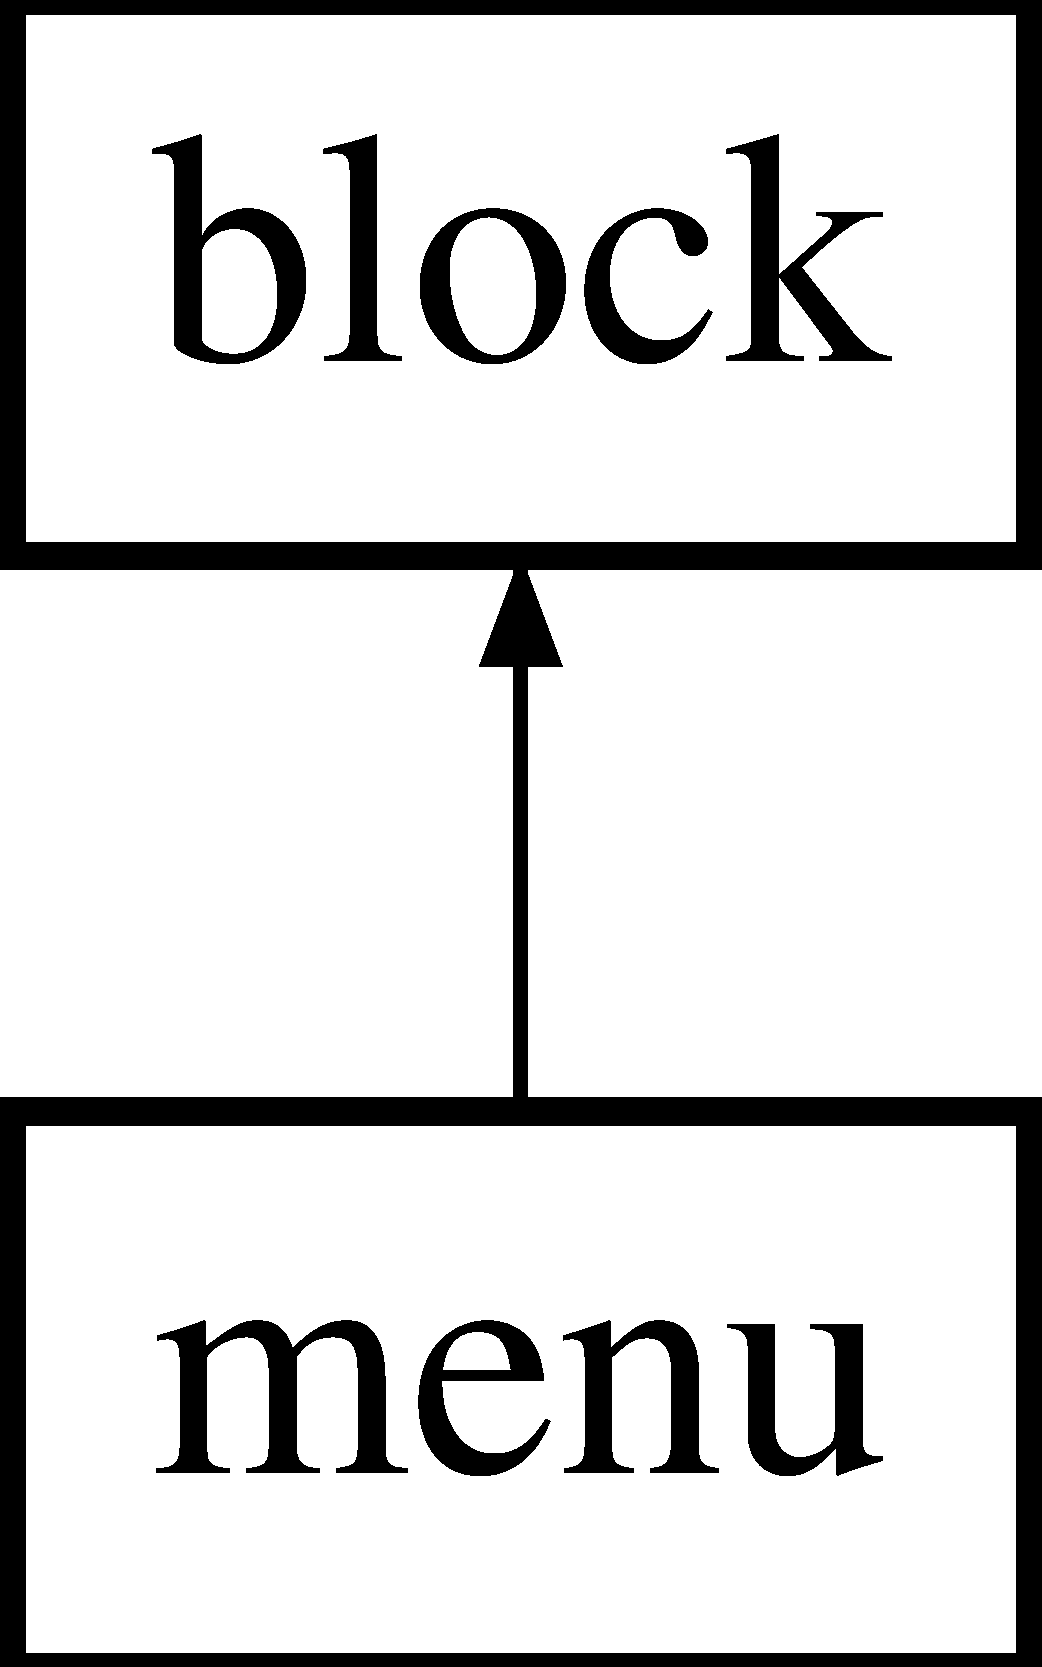
\includegraphics[height=2.000000cm]{classmenu}
\end{center}
\end{figure}
\subsection*{\-Métodos públicos}
\begin{DoxyCompactItemize}
\item 
\hypertarget{classmenu_abadf0a36d865e21da5799e2b9268edfa}{{\bfseries display} ()}\label{classmenu_abadf0a36d865e21da5799e2b9268edfa}

\end{DoxyCompactItemize}


\subsection{\-Descripción detallada}


\-Definición en la línea 5 del archivo menu.\-php.



\-La documentación para esta clase fue generada a partir del siguiente fichero\-:\begin{DoxyCompactItemize}
\item 
menu.\-php\end{DoxyCompactItemize}

\hypertarget{classmenuadmin}{\section{\-Referencia de la \-Clase menuadmin}
\label{classmenuadmin}\index{menuadmin@{menuadmin}}
}
\-Diagrama de herencias de menuadmin\begin{figure}[H]
\begin{center}
\leavevmode
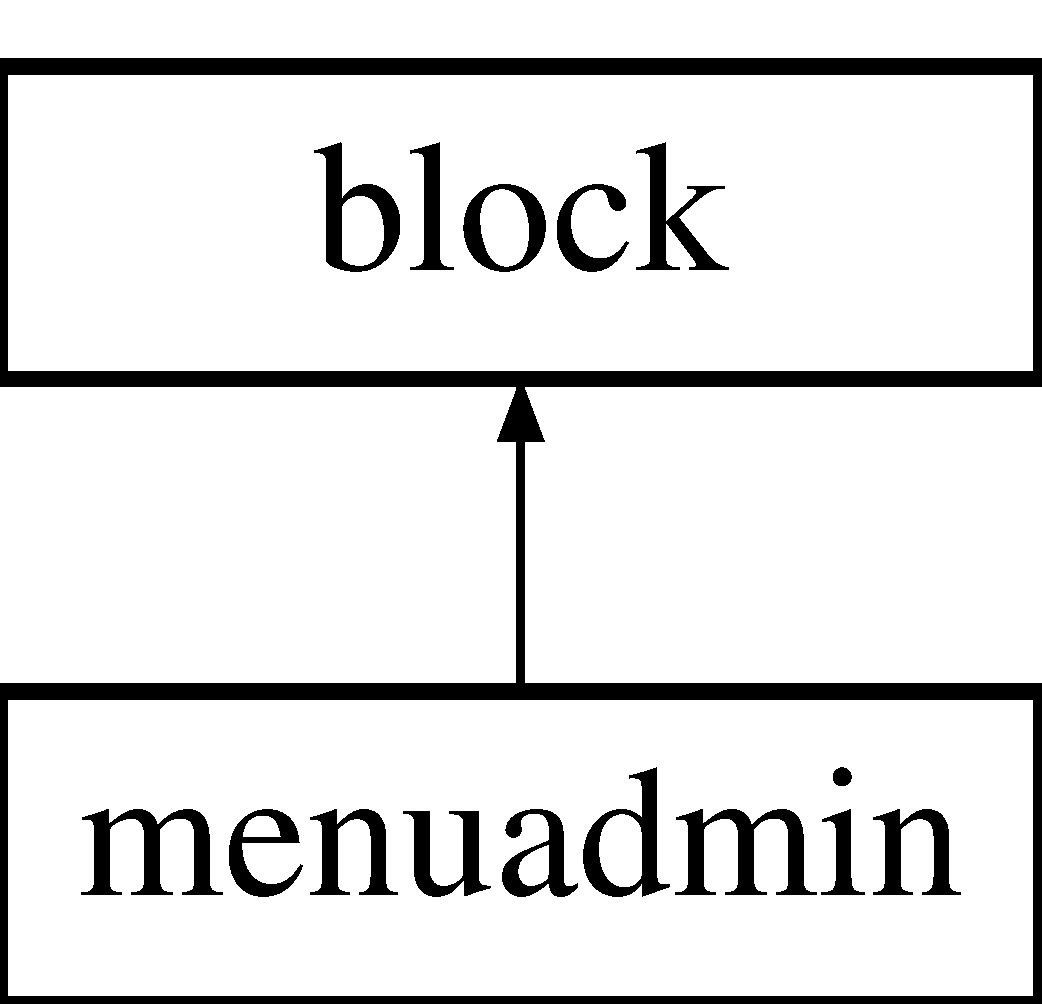
\includegraphics[height=2.000000cm]{classmenuadmin}
\end{center}
\end{figure}
\subsection*{\-Métodos públicos}
\begin{DoxyCompactItemize}
\item 
\hypertarget{classmenuadmin_a2df0d677d2ebbb3586176372ccd4b009}{{\bfseries display} ()}\label{classmenuadmin_a2df0d677d2ebbb3586176372ccd4b009}

\end{DoxyCompactItemize}


\subsection{\-Descripción detallada}


\-Definición en la línea 5 del archivo menuadmin.\-php.



\-La documentación para esta clase fue generada a partir del siguiente fichero\-:\begin{DoxyCompactItemize}
\item 
admin/menuadmin.\-php\end{DoxyCompactItemize}

\hypertarget{classMyXml}{\section{\-Referencia de la \-Clase \-My\-Xml}
\label{classMyXml}\index{\-My\-Xml@{\-My\-Xml}}
}
\-Diagrama de herencias de \-My\-Xml\begin{figure}[H]
\begin{center}
\leavevmode
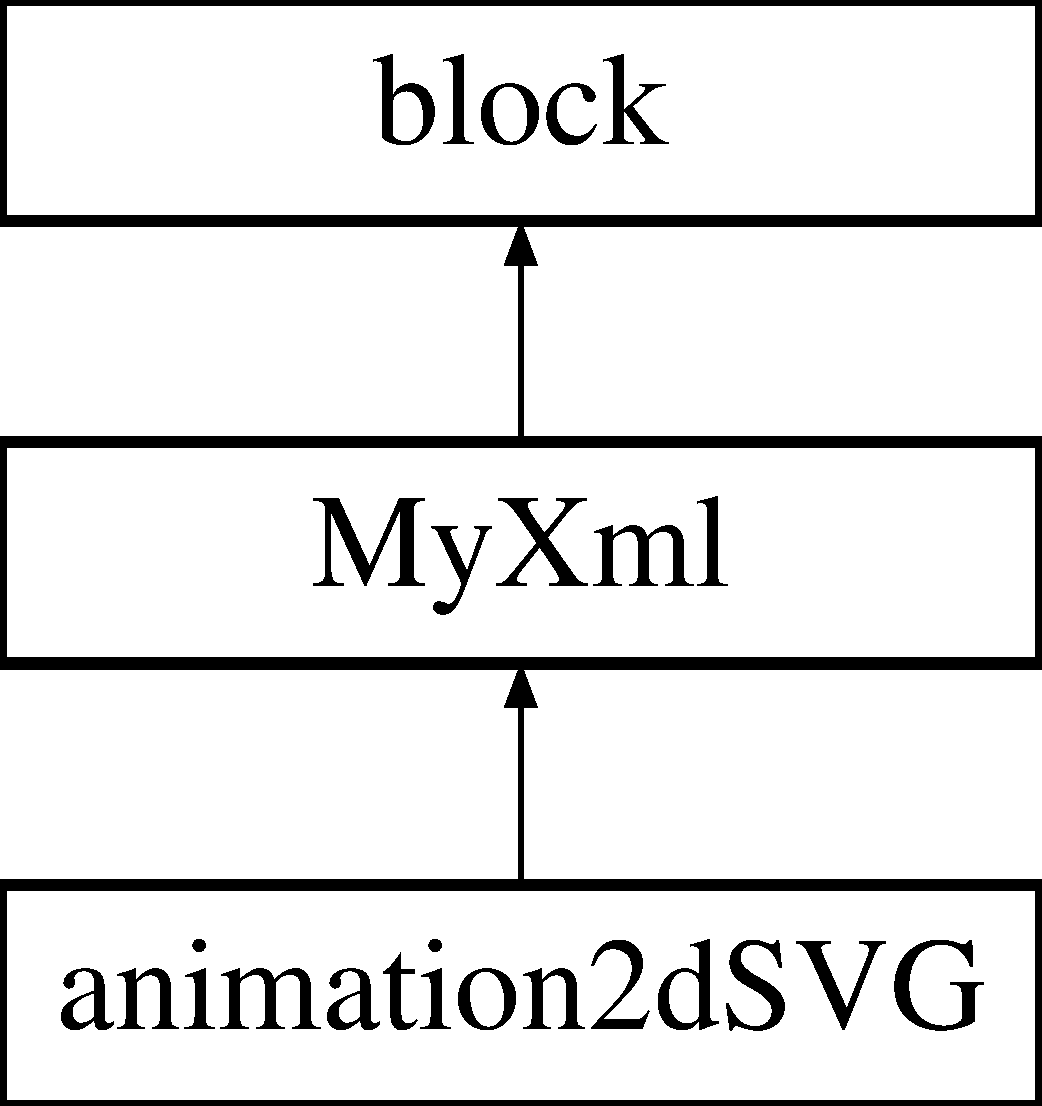
\includegraphics[height=3.000000cm]{classMyXml}
\end{center}
\end{figure}
\subsection*{\-Métodos públicos}
\begin{DoxyCompactItemize}
\item 
\hypertarget{classMyXml_a3a5ea00bcb3df045d4139e2a235f8a22}{{\bfseries read\-Xml\-File} (\$fn)}\label{classMyXml_a3a5ea00bcb3df045d4139e2a235f8a22}

\item 
\hypertarget{classMyXml_af4f787faf6b54c376a570f692c52051d}{{\bfseries read\-Xml\-String} (\$xmlstr)}\label{classMyXml_af4f787faf6b54c376a570f692c52051d}

\item 
\hypertarget{classMyXml_af11dcf960ad0c75397ebf347d879c388}{{\bfseries tab} (\$tab)}\label{classMyXml_af11dcf960ad0c75397ebf347d879c388}

\item 
\hypertarget{classMyXml_a055ad33e1423261776210b0676e09ab3}{{\bfseries write\-Xml\-File} (\$fn)}\label{classMyXml_a055ad33e1423261776210b0676e09ab3}

\item 
\hypertarget{classMyXml_a492e0260476d66ca7e2708f50c1c84da}{{\bfseries write\-Xml\-String} ()}\label{classMyXml_a492e0260476d66ca7e2708f50c1c84da}

\item 
\hypertarget{classMyXml_a276fe0044f6d61474726e3a2751908f8}{{\bfseries clean\-String} (\$strin)}\label{classMyXml_a276fe0044f6d61474726e3a2751908f8}

\item 
\hypertarget{classMyXml_afb7ddb2e7374cd53666ecf385e5d5be5}{{\bfseries write\-Node\-Attributes} (\$node, \$tab)}\label{classMyXml_afb7ddb2e7374cd53666ecf385e5d5be5}

\item 
\hypertarget{classMyXml_a7fc15bbfded7db0bd48351960e5e845d}{{\bfseries write\-Node\-Value} (\$node)}\label{classMyXml_a7fc15bbfded7db0bd48351960e5e845d}

\item 
\hypertarget{classMyXml_a76077b211289f21055bf6b3aecc0c8c8}{{\bfseries write\-Node\-String} (\$type, \$node, \$tab)}\label{classMyXml_a76077b211289f21055bf6b3aecc0c8c8}

\item 
\hypertarget{classMyXml_a5e8568f0e01d562a5e26813b46c31b2f}{{\bfseries insert\-Node} (\&\$node, \$type, \$subnode)}\label{classMyXml_a5e8568f0e01d562a5e26813b46c31b2f}

\item 
\hypertarget{classMyXml_ac6bd925dadb3166b08ac5e2cf17c59ef}{{\bfseries remove\-Node} (\&\$node, \$type, \$subnode)}\label{classMyXml_ac6bd925dadb3166b08ac5e2cf17c59ef}

\end{DoxyCompactItemize}
\subsection*{\-Atributos públicos}
\begin{DoxyCompactItemize}
\item 
\hypertarget{classMyXml_a2f675194b628cef67cea0fecbc213be5}{{\bfseries \$tree}}\label{classMyXml_a2f675194b628cef67cea0fecbc213be5}

\end{DoxyCompactItemize}


\subsection{\-Descripción detallada}


\-Definición en la línea 4 del archivo \-My\-Xml.\-php.



\-La documentación para esta clase fue generada a partir del siguiente fichero\-:\begin{DoxyCompactItemize}
\item 
\-My\-Xml.\-php\end{DoxyCompactItemize}

\hypertarget{classoutputs}{\section{\-Referencia de la \-Clase outputs}
\label{classoutputs}\index{outputs@{outputs}}
}
\-Diagrama de herencias de outputs\begin{figure}[H]
\begin{center}
\leavevmode
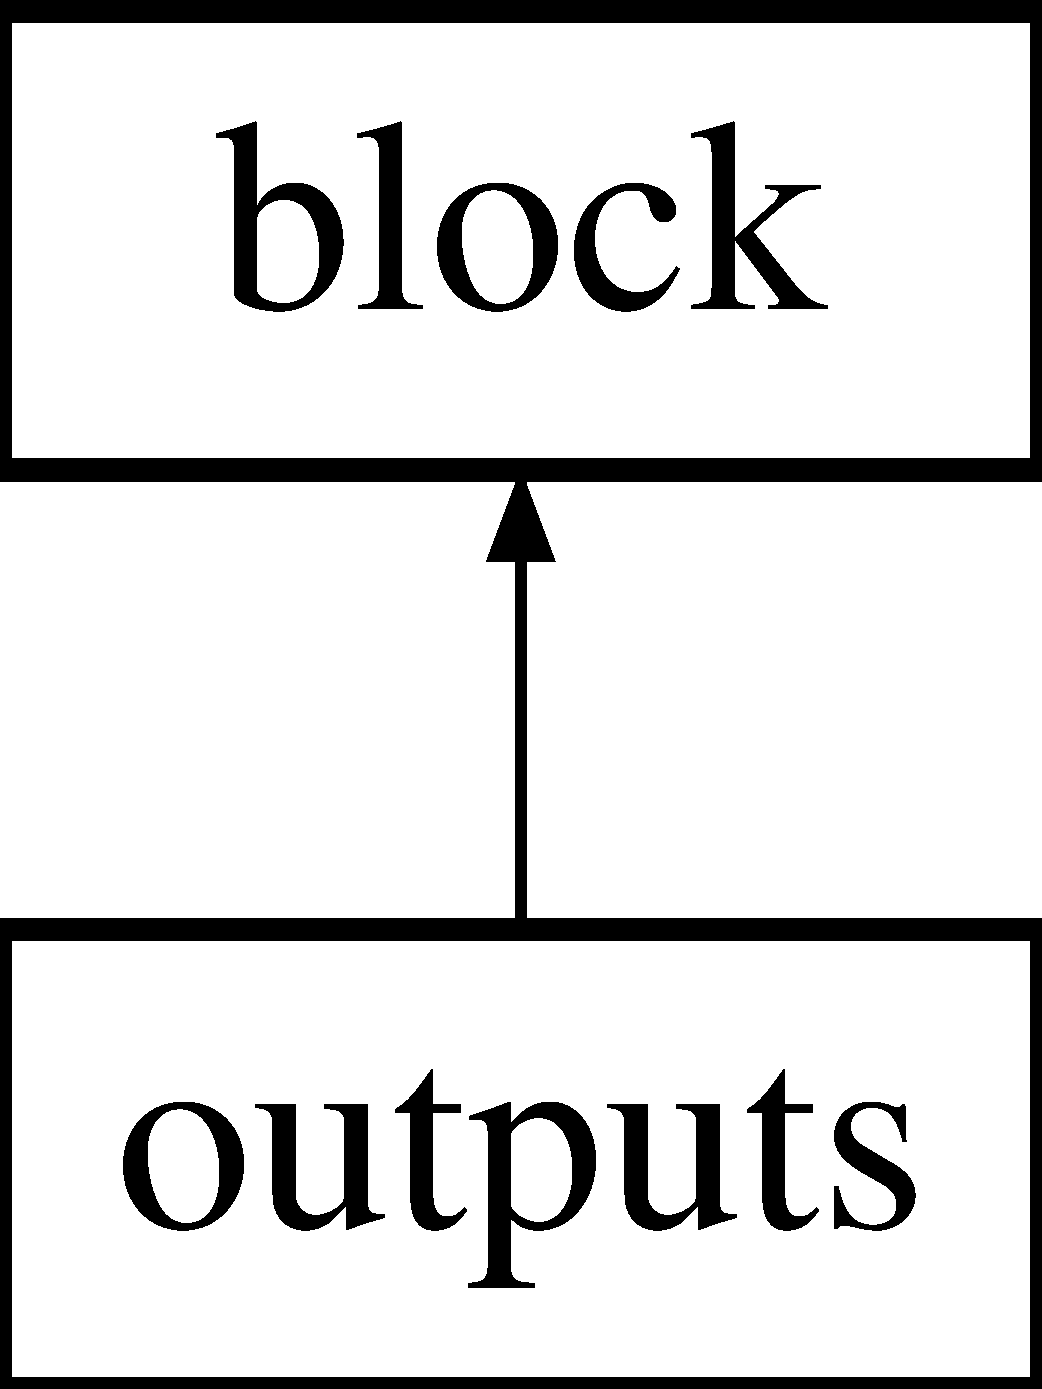
\includegraphics[height=2.000000cm]{classoutputs}
\end{center}
\end{figure}
\subsection*{\-Métodos públicos}
\begin{DoxyCompactItemize}
\item 
\hypertarget{classoutputs_ab48bb5d47938c85da5891c1250c18a5f}{{\bfseries display} ()}\label{classoutputs_ab48bb5d47938c85da5891c1250c18a5f}

\end{DoxyCompactItemize}


\subsection{\-Descripción detallada}


\-Definición en la línea 4 del archivo outputs.\-php.



\-La documentación para esta clase fue generada a partir del siguiente fichero\-:\begin{DoxyCompactItemize}
\item 
outputs.\-php\end{DoxyCompactItemize}

\hypertarget{classplots}{\section{\-Referencia de la \-Clase plots}
\label{classplots}\index{plots@{plots}}
}
\-Diagrama de herencias de plots\begin{figure}[H]
\begin{center}
\leavevmode
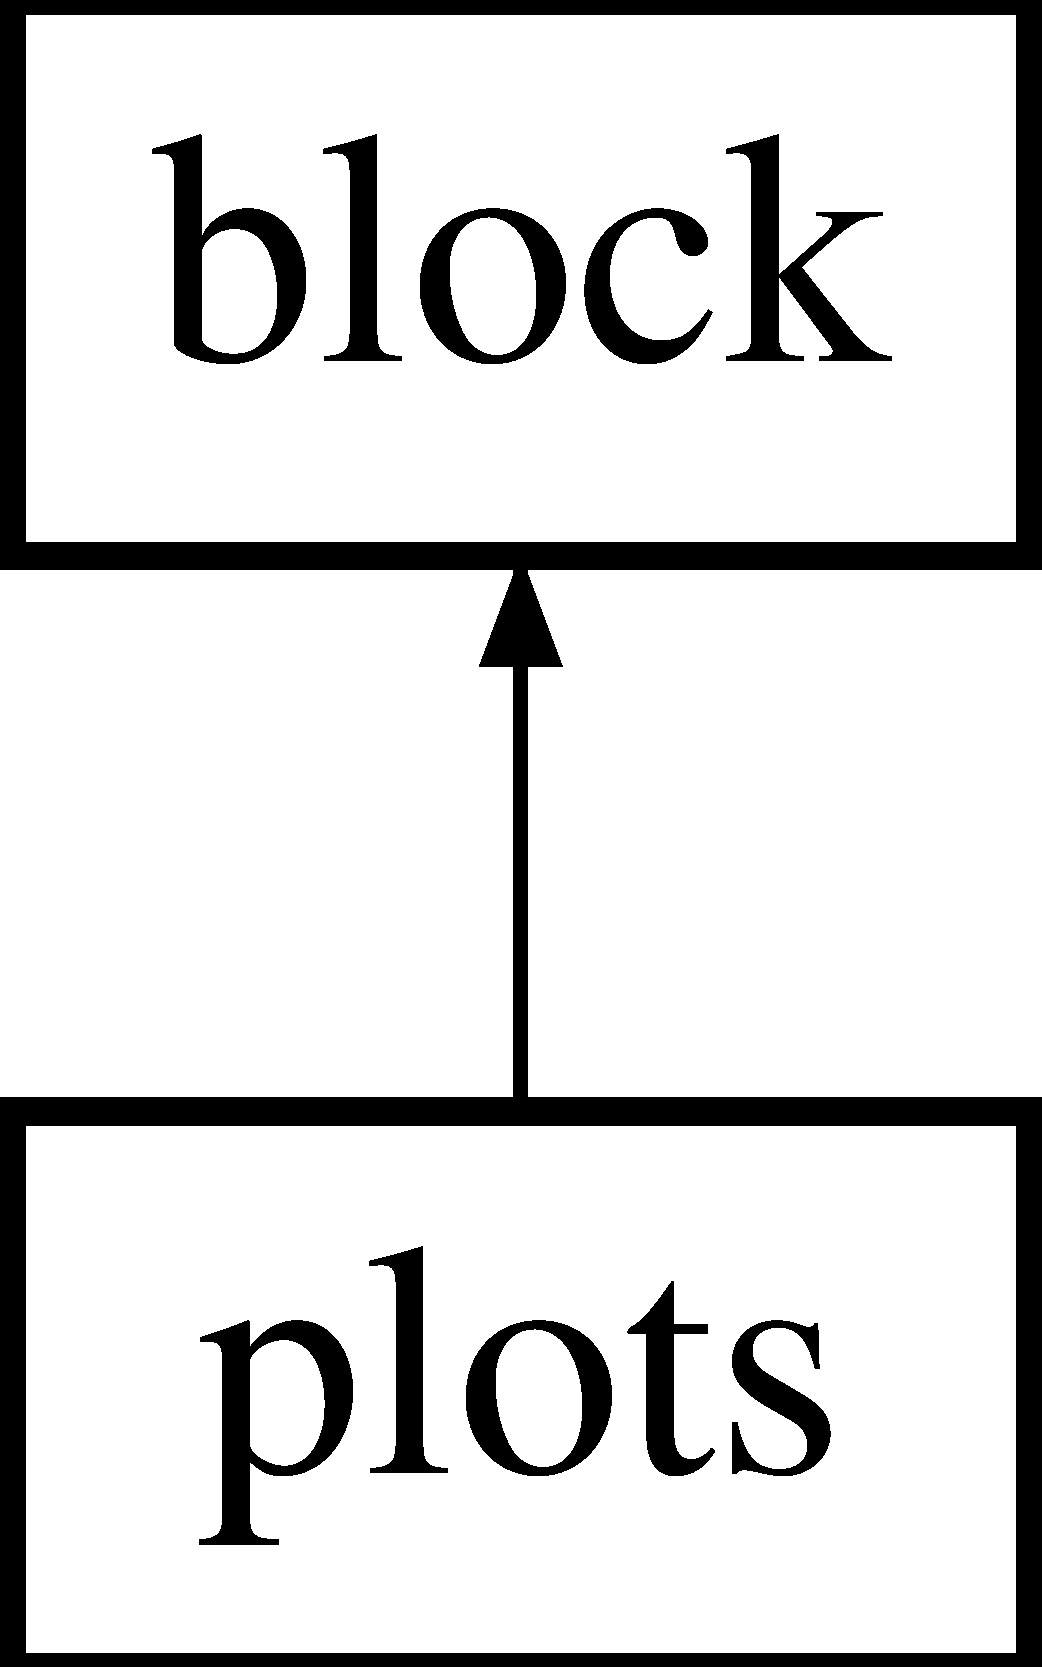
\includegraphics[height=2.000000cm]{classplots}
\end{center}
\end{figure}
\subsection*{\-Métodos públicos}
\begin{DoxyCompactItemize}
\item 
\hypertarget{classplots_a2bbdf8344df94f2b1cfb51d6144d95f7}{{\bfseries display\-Plot} (\$plot)}\label{classplots_a2bbdf8344df94f2b1cfb51d6144d95f7}

\item 
\hypertarget{classplots_a96aa342680d985e274c53cddd3e39978}{{\bfseries display} ()}\label{classplots_a96aa342680d985e274c53cddd3e39978}

\end{DoxyCompactItemize}


\subsection{\-Descripción detallada}


\-Definición en la línea 6 del archivo plots.\-php.



\-La documentación para esta clase fue generada a partir del siguiente fichero\-:\begin{DoxyCompactItemize}
\item 
plots.\-php\end{DoxyCompactItemize}

\hypertarget{classsessionManager}{}\section{Referencia de la Clase session\+Manager}
\label{classsessionManager}\index{session\+Manager@{session\+Manager}}
Diagrama de herencias de session\+Manager\begin{figure}[H]
\begin{center}
\leavevmode
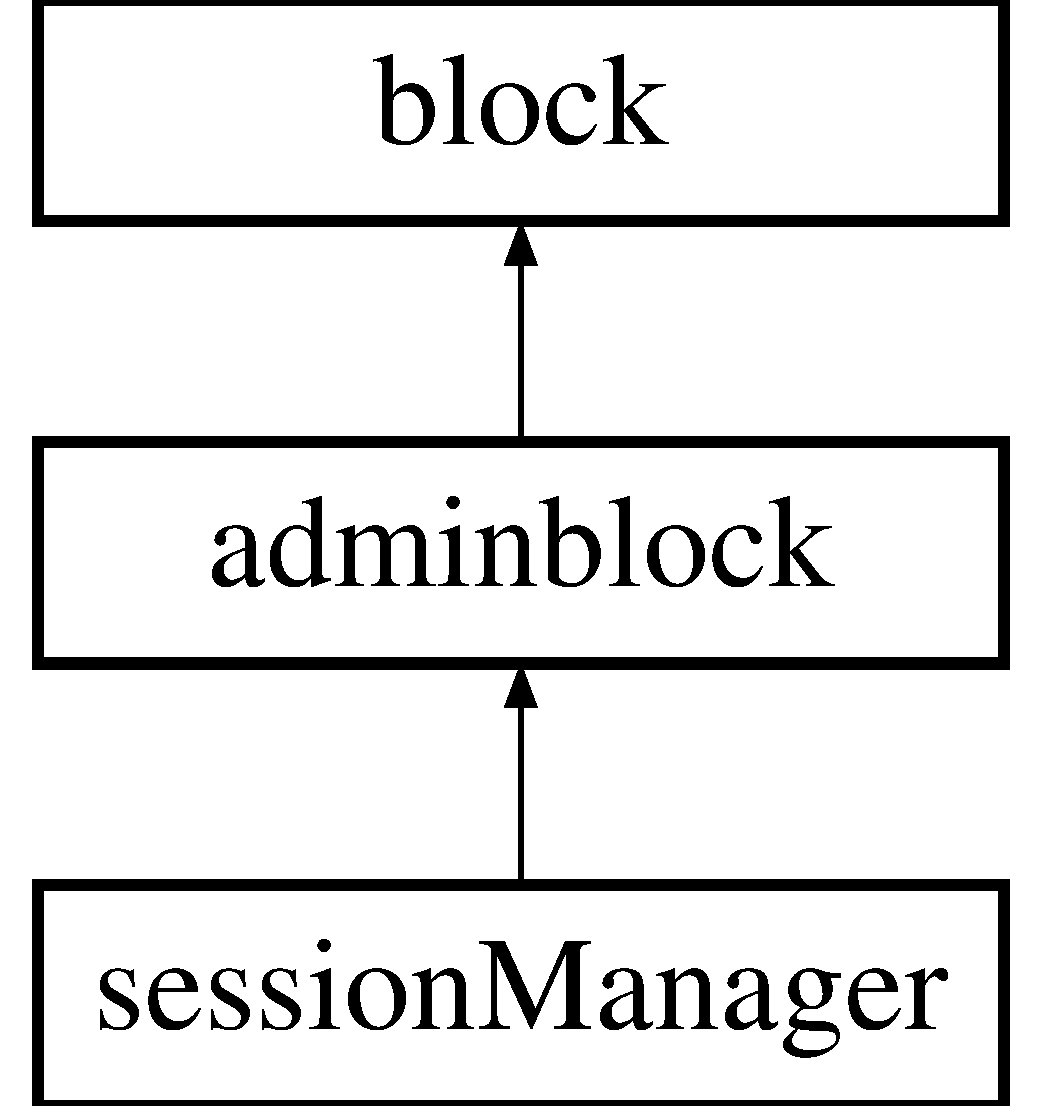
\includegraphics[height=3.000000cm]{classsessionManager}
\end{center}
\end{figure}
\subsection*{Métodos públicos}
\begin{DoxyCompactItemize}
\item 
\mbox{\Hypertarget{classsessionManager_a341e75413ef5e07e6d59f49e7b1845db}\label{classsessionManager_a341e75413ef5e07e6d59f49e7b1845db}} 
{\bfseries verify} ()
\end{DoxyCompactItemize}
\subsection*{Otros miembros heredados}


\subsection{Descripción detallada}


Definición en la línea 4 del archivo session.\+php.



La documentación para esta clase fue generada a partir del siguiente fichero\+:\begin{DoxyCompactItemize}
\item 
/home/ogduartev/public\+\_\+html/unvl-\/\+Git\+Hub/\+U\+N\+Virtual\+Lab/admin/session.\+php\end{DoxyCompactItemize}

\hypertarget{classsimulator}{}\section{Referencia de la Clase simulator}
\label{classsimulator}\index{simulator@{simulator}}
Diagrama de herencias de simulator\begin{figure}[H]
\begin{center}
\leavevmode
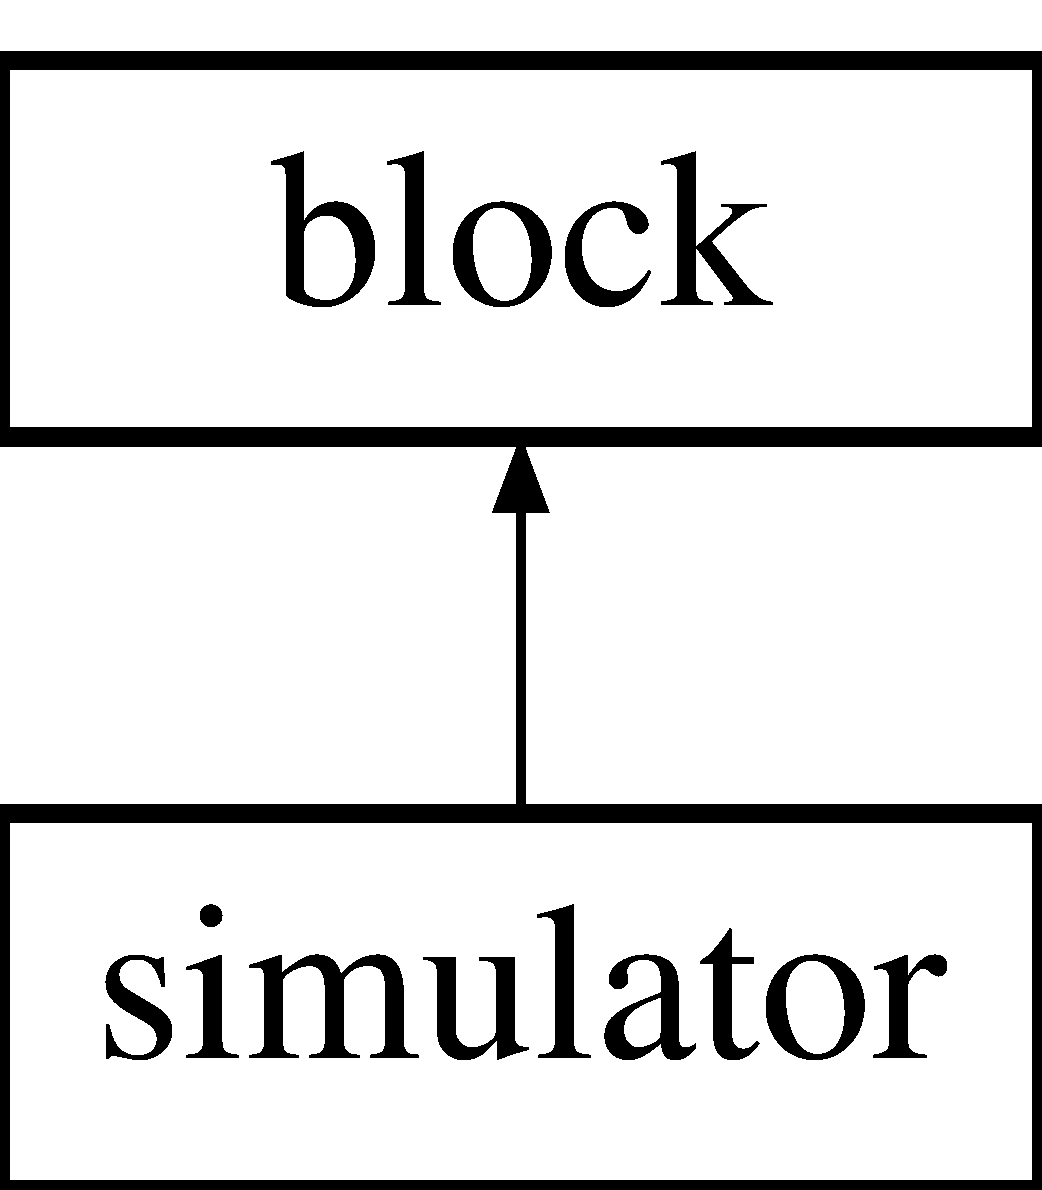
\includegraphics[height=2.000000cm]{classsimulator}
\end{center}
\end{figure}
\subsection*{Métodos públicos}
\begin{DoxyCompactItemize}
\item 
\mbox{\Hypertarget{classsimulator_a497dea92712b83b74a4b14a451a325bf}\label{classsimulator_a497dea92712b83b74a4b14a451a325bf}} 
{\bfseries exe\+File\+Name} (\$model\+\_\+id)
\item 
\mbox{\Hypertarget{classsimulator_aed1bde74d630efcdd550be8e2312f332}\label{classsimulator_aed1bde74d630efcdd550be8e2312f332}} 
{\bfseries read\+Init\+Xml} (\$fn)
\item 
\mbox{\Hypertarget{classsimulator_ad4b5ce28959a3b2d8b139de21b12e04b}\label{classsimulator_ad4b5ce28959a3b2d8b139de21b12e04b}} 
{\bfseries find\+Modelica\+Name} (\$var\+\_\+id)
\item 
\mbox{\Hypertarget{classsimulator_a6d760375c95203a02545a9c5838505ae}\label{classsimulator_a6d760375c95203a02545a9c5838505ae}} 
{\bfseries change\+Output\+Filter} (\$model\+\_\+id)
\item 
\mbox{\Hypertarget{classsimulator_a8e062f80da89131cfe9e64e91f96bc97}\label{classsimulator_a8e062f80da89131cfe9e64e91f96bc97}} 
{\bfseries change\+Values} ()
\item 
\mbox{\Hypertarget{classsimulator_a5548efec5d30fb22a9087f6f2f98b38f}\label{classsimulator_a5548efec5d30fb22a9087f6f2f98b38f}} 
{\bfseries tab} (\$tab)
\item 
\mbox{\Hypertarget{classsimulator_abac7c67e94f6f8838929470aba00b855}\label{classsimulator_abac7c67e94f6f8838929470aba00b855}} 
{\bfseries encabezado\+Xml} ()
\item 
\mbox{\Hypertarget{classsimulator_a0caf039e06db381e1ca2b333645f6289}\label{classsimulator_a0caf039e06db381e1ca2b333645f6289}} 
{\bfseries atributos\+Xml} (\$att, \$tab)
\item 
\mbox{\Hypertarget{classsimulator_ae540c1deb78b2052455f203a75b4ff20}\label{classsimulator_ae540c1deb78b2052455f203a75b4ff20}} 
{\bfseries cadena\+Tipo} (\$t, \$xml, \$tab)
\item 
\mbox{\Hypertarget{classsimulator_a71e23d57a0e055a2b6b59770271ce16f}\label{classsimulator_a71e23d57a0e055a2b6b59770271ce16f}} 
{\bfseries cadena\+Scalar\+Xml} (\$xml, \$tab)
\item 
\mbox{\Hypertarget{classsimulator_a8576fab3134387fccbd6678ebbceac47}\label{classsimulator_a8576fab3134387fccbd6678ebbceac47}} 
{\bfseries scalar\+Vars\+Xml} (\$xml, \$tab)
\item 
\mbox{\Hypertarget{classsimulator_a52f49eb756fe2ee3238fccd1017bacb1}\label{classsimulator_a52f49eb756fe2ee3238fccd1017bacb1}} 
{\bfseries cadena\+Model\+Xml} (\$xml, \$tab)
\item 
\mbox{\Hypertarget{classsimulator_a1a13b97820999ff1e9aedd046d03f8aa}\label{classsimulator_a1a13b97820999ff1e9aedd046d03f8aa}} 
{\bfseries cadena\+Exp\+Xml} (\$xml, \$tab)
\item 
\mbox{\Hypertarget{classsimulator_a5d5ccd8544c32ebd959e09ca16133a0c}\label{classsimulator_a5d5ccd8544c32ebd959e09ca16133a0c}} 
{\bfseries cadena\+Fmi\+Xml} (\$xml, \$tab)
\item 
\mbox{\Hypertarget{classsimulator_af9b860cbf6812dfb766be1bfe8b9e741}\label{classsimulator_af9b860cbf6812dfb766be1bfe8b9e741}} 
{\bfseries write\+Init\+Xml} (\$fn, \$tab)
\item 
\mbox{\Hypertarget{classsimulator_a5167700851518332f76a993b14875364}\label{classsimulator_a5167700851518332f76a993b14875364}} 
{\bfseries run\+Simulation} (\$model\+\_\+id, \$exename, \$tmp\+Init\+File)
\item 
\mbox{\Hypertarget{classsimulator_ac2a0fdfba4df28bdcd947e691e09eafd}\label{classsimulator_ac2a0fdfba4df28bdcd947e691e09eafd}} 
{\bfseries simulate} (\$model\+\_\+id)
\end{DoxyCompactItemize}
\subsection*{Atributos públicos}
\begin{DoxyCompactItemize}
\item 
\mbox{\Hypertarget{classsimulator_acab8cf77a5b3f2863119c5a96f613785}\label{classsimulator_acab8cf77a5b3f2863119c5a96f613785}} 
{\bfseries \$\+X\+ML}
\end{DoxyCompactItemize}


\subsection{Descripción detallada}


Definición en la línea 5 del archivo simulator.\+php.



La documentación para esta clase fue generada a partir del siguiente fichero\+:\begin{DoxyCompactItemize}
\item 
/home/ogduartev/public\+\_\+html/unvl-\/\+Git\+Hub/\+U\+N\+Virtual\+Lab/simulator.\+php\end{DoxyCompactItemize}

\hypertarget{classSVGplot}{}\section{Referencia de la Clase S\+V\+Gplot}
\label{classSVGplot}\index{S\+V\+Gplot@{S\+V\+Gplot}}
Diagrama de herencias de S\+V\+Gplot\begin{figure}[H]
\begin{center}
\leavevmode
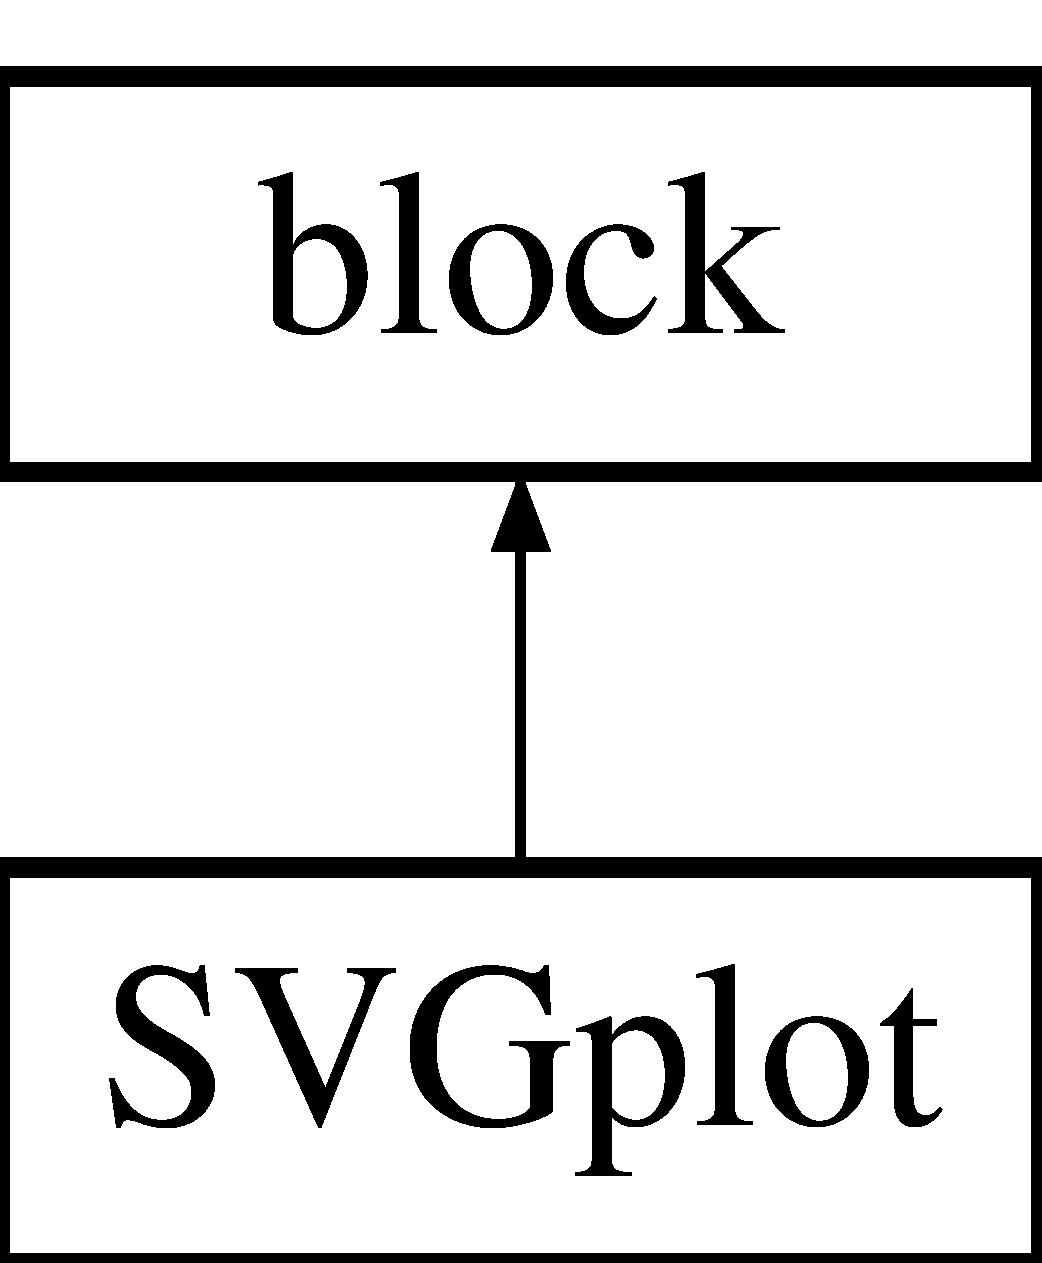
\includegraphics[height=2.000000cm]{classSVGplot}
\end{center}
\end{figure}
\subsection*{Métodos públicos}
\begin{DoxyCompactItemize}
\item 
\mbox{\Hypertarget{classSVGplot_adccc27accb9425cfd277caa7a294706f}\label{classSVGplot_adccc27accb9425cfd277caa7a294706f}} 
{\bfseries S\+V\+Gplot} ()
\item 
\mbox{\Hypertarget{classSVGplot_aaf1c0515200e6695c63c3e133d9cb043}\label{classSVGplot_aaf1c0515200e6695c63c3e133d9cb043}} 
{\bfseries settings} (\$settings)
\item 
\mbox{\Hypertarget{classSVGplot_a8462b445cdf45abf633cfcde7a9aa1d1}\label{classSVGplot_a8462b445cdf45abf633cfcde7a9aa1d1}} 
{\bfseries title} ()
\item 
\mbox{\Hypertarget{classSVGplot_aae9aad60aab30a75bb12c965a248aba5}\label{classSVGplot_aae9aad60aab30a75bb12c965a248aba5}} 
{\bfseries grid} ()
\item 
\mbox{\Hypertarget{classSVGplot_a86654740ec88200e4ea1b1b1d5c6614f}\label{classSVGplot_a86654740ec88200e4ea1b1b1d5c6614f}} 
{\bfseries curves} ()
\item 
\mbox{\Hypertarget{classSVGplot_a55a763e6eec15d62f92e3dead44a6c16}\label{classSVGplot_a55a763e6eec15d62f92e3dead44a6c16}} 
{\bfseries frame} ()
\item 
\mbox{\Hypertarget{classSVGplot_af6a5009609ae6646d09ee8dfe9613381}\label{classSVGplot_af6a5009609ae6646d09ee8dfe9613381}} 
{\bfseries str\+Num} (\$x)
\item 
\mbox{\Hypertarget{classSVGplot_a007101274ca32181ede8b05b82df39d7}\label{classSVGplot_a007101274ca32181ede8b05b82df39d7}} 
{\bfseries tagH} ()
\item 
\mbox{\Hypertarget{classSVGplot_ab0e5cad94e279789622b59ab6b89d879}\label{classSVGplot_ab0e5cad94e279789622b59ab6b89d879}} 
{\bfseries tagV} ()
\item 
\mbox{\Hypertarget{classSVGplot_aa46a4001e171f238db3c4e83359536d0}\label{classSVGplot_aa46a4001e171f238db3c4e83359536d0}} 
{\bfseries plot} ()
\item 
\mbox{\Hypertarget{classSVGplot_a8147cc7bc479c75960ba276a79376759}\label{classSVGplot_a8147cc7bc479c75960ba276a79376759}} 
{\bfseries legend} ()
\item 
\mbox{\Hypertarget{classSVGplot_af0bb4c5ecb4d048ecc0e9d7b61415a9e}\label{classSVGplot_af0bb4c5ecb4d048ecc0e9d7b61415a9e}} 
{\bfseries display} ()
\item 
\mbox{\Hypertarget{classSVGplot_a2d15939112d74e32ce1800633b3a6ebc}\label{classSVGplot_a2d15939112d74e32ce1800633b3a6ebc}} 
{\bfseries data} (\$plot, \$resfile)
\end{DoxyCompactItemize}
\subsection*{Atributos públicos}
\begin{DoxyCompactItemize}
\item 
\mbox{\Hypertarget{classSVGplot_afbdc38c2ed4d610287a5c710c8e4d94b}\label{classSVGplot_afbdc38c2ed4d610287a5c710c8e4d94b}} 
{\bfseries \$svg\+Str} =\char`\"{}\char`\"{}
\item 
\mbox{\Hypertarget{classSVGplot_ab4b92d2b39041d690561c6e252d1d809}\label{classSVGplot_ab4b92d2b39041d690561c6e252d1d809}} 
{\bfseries \$total\+Width} =300
\item 
\mbox{\Hypertarget{classSVGplot_a69a1c131f1fe715f3aba3a5518cdb243}\label{classSVGplot_a69a1c131f1fe715f3aba3a5518cdb243}} 
{\bfseries \$total\+Height} =200
\item 
\mbox{\Hypertarget{classSVGplot_ad87fa0cf5b64b9546f0698350b8200e7}\label{classSVGplot_ad87fa0cf5b64b9546f0698350b8200e7}} 
{\bfseries \$title\+Height} =10
\item 
\mbox{\Hypertarget{classSVGplot_a8727575cf82ab9edb4351ce00f502024}\label{classSVGplot_a8727575cf82ab9edb4351ce00f502024}} 
{\bfseries \$plot\+Height} =80
\item 
\mbox{\Hypertarget{classSVGplot_aca9c01c3c068bd2f9d231c281b250627}\label{classSVGplot_aca9c01c3c068bd2f9d231c281b250627}} 
{\bfseries \$legend\+Height} =5
\item 
\mbox{\Hypertarget{classSVGplot_a49f887d1455897db25d0362c9b0a3a09}\label{classSVGplot_a49f887d1455897db25d0362c9b0a3a09}} 
{\bfseries \$frame\+PositionX} =20
\item 
\mbox{\Hypertarget{classSVGplot_a0240f4bebcef331b76ed3c68cd4e7c46}\label{classSVGplot_a0240f4bebcef331b76ed3c68cd4e7c46}} 
{\bfseries \$frame\+PositionY} =5
\item 
\mbox{\Hypertarget{classSVGplot_aaa53103b66970ef7d13ee5ee15fa6f3a}\label{classSVGplot_aaa53103b66970ef7d13ee5ee15fa6f3a}} 
{\bfseries \$frame\+Width} =75
\item 
\mbox{\Hypertarget{classSVGplot_a2967f6c2f9c5070bb5723c16b53bd8cf}\label{classSVGplot_a2967f6c2f9c5070bb5723c16b53bd8cf}} 
{\bfseries \$frame\+Height} =85
\item 
\mbox{\Hypertarget{classSVGplot_a5aee502fb832abcb7ca279ac74daac3b}\label{classSVGplot_a5aee502fb832abcb7ca279ac74daac3b}} 
{\bfseries \$tag\+Height} =10
\item 
\mbox{\Hypertarget{classSVGplot_adca0e187cce2c1613aeabd0d8040d971}\label{classSVGplot_adca0e187cce2c1613aeabd0d8040d971}} 
{\bfseries \$tag\+Width} =20
\item 
\mbox{\Hypertarget{classSVGplot_a6d7b21d8825604b8c5dd543179292760}\label{classSVGplot_a6d7b21d8825604b8c5dd543179292760}} 
{\bfseries \$legend\+Separation} =20
\item 
\mbox{\Hypertarget{classSVGplot_adcb4d04fdba2845716cc063cd1c81598}\label{classSVGplot_adcb4d04fdba2845716cc063cd1c81598}} 
{\bfseries \$title} =\char`\"{}\char`\"{}
\item 
\mbox{\Hypertarget{classSVGplot_acf2db453a81de4e1aee086ccddd9053a}\label{classSVGplot_acf2db453a81de4e1aee086ccddd9053a}} 
{\bfseries \$description} =\char`\"{}\char`\"{}
\item 
\mbox{\Hypertarget{classSVGplot_a1a284a2d15bbc78f9a42ab9c02ee4405}\label{classSVGplot_a1a284a2d15bbc78f9a42ab9c02ee4405}} 
{\bfseries \$gridX} =5
\item 
\mbox{\Hypertarget{classSVGplot_a6a3da9c6b781e85dfb536a5ba0a7b4e5}\label{classSVGplot_a6a3da9c6b781e85dfb536a5ba0a7b4e5}} 
{\bfseries \$gridY} =3
\item 
\mbox{\Hypertarget{classSVGplot_a2afb9baba9be91235a417d64b626a1a8}\label{classSVGplot_a2afb9baba9be91235a417d64b626a1a8}} 
{\bfseries \$autoscaleX} =\textquotesingle{}1\textquotesingle{}
\item 
\mbox{\Hypertarget{classSVGplot_a879d5c10d138b0550206417e94ce654b}\label{classSVGplot_a879d5c10d138b0550206417e94ce654b}} 
{\bfseries \$autoscaleY} =\textquotesingle{}1\textquotesingle{}
\item 
\mbox{\Hypertarget{classSVGplot_a5eb64028c5cae66b06ce65039df3bfc7}\label{classSVGplot_a5eb64028c5cae66b06ce65039df3bfc7}} 
{\bfseries \$minX} =0.\+0
\item 
\mbox{\Hypertarget{classSVGplot_afb7089f298f05a9d9337b79a5ecbaecb}\label{classSVGplot_afb7089f298f05a9d9337b79a5ecbaecb}} 
{\bfseries \$maxX} =1.\+0
\item 
\mbox{\Hypertarget{classSVGplot_a1cf6d7665187cdcff7721f4a41b2590d}\label{classSVGplot_a1cf6d7665187cdcff7721f4a41b2590d}} 
{\bfseries \$minY} =0.\+0
\item 
\mbox{\Hypertarget{classSVGplot_a3e917ac1e30762bb7fc99ed715a36ab7}\label{classSVGplot_a3e917ac1e30762bb7fc99ed715a36ab7}} 
{\bfseries \$maxY} =1.\+0
\item 
\mbox{\Hypertarget{classSVGplot_ae31b72045889d0bf812ae835f836cdd8}\label{classSVGplot_ae31b72045889d0bf812ae835f836cdd8}} 
{\bfseries \$data}
\item 
\mbox{\Hypertarget{classSVGplot_a8dbfedecb97d3c82c30a2b43d4b57c79}\label{classSVGplot_a8dbfedecb97d3c82c30a2b43d4b57c79}} 
{\bfseries \$colors}
\item 
\mbox{\Hypertarget{classSVGplot_a8893ea8511edcdad8a90cace54db09b1}\label{classSVGplot_a8893ea8511edcdad8a90cace54db09b1}} 
{\bfseries \$legends}
\item 
\mbox{\Hypertarget{classSVGplot_a8d000e306c896835b1e8aab693e1772a}\label{classSVGplot_a8d000e306c896835b1e8aab693e1772a}} 
{\bfseries \$units}
\item 
\mbox{\Hypertarget{classSVGplot_a60a60e1c751277eb8db37bf9fdc60c79}\label{classSVGplot_a60a60e1c751277eb8db37bf9fdc60c79}} 
{\bfseries \$descriptions}
\item 
\mbox{\Hypertarget{classSVGplot_aef827b465ef1dbc6c2e3dd72496eba7e}\label{classSVGplot_aef827b465ef1dbc6c2e3dd72496eba7e}} 
{\bfseries \$legendH} =\char`\"{}\char`\"{}
\item 
\mbox{\Hypertarget{classSVGplot_a03724d0202bd3c8a1ee866deea738377}\label{classSVGplot_a03724d0202bd3c8a1ee866deea738377}} 
{\bfseries \$unitsH} =\char`\"{}\char`\"{}
\end{DoxyCompactItemize}


\subsection{Descripción detallada}


Definición en la línea 5 del archivo svgplot.\+php.



La documentación para esta clase fue generada a partir del siguiente fichero\+:\begin{DoxyCompactItemize}
\item 
/home/ogduartev/public\+\_\+html/unvl-\/\+Git\+Hub/\+U\+N\+Virtual\+Lab/svgplot.\+php\end{DoxyCompactItemize}

\hypertarget{classtables}{\section{\-Referencia de la \-Clase tables}
\label{classtables}\index{tables@{tables}}
}
\-Diagrama de herencias de tables\begin{figure}[H]
\begin{center}
\leavevmode
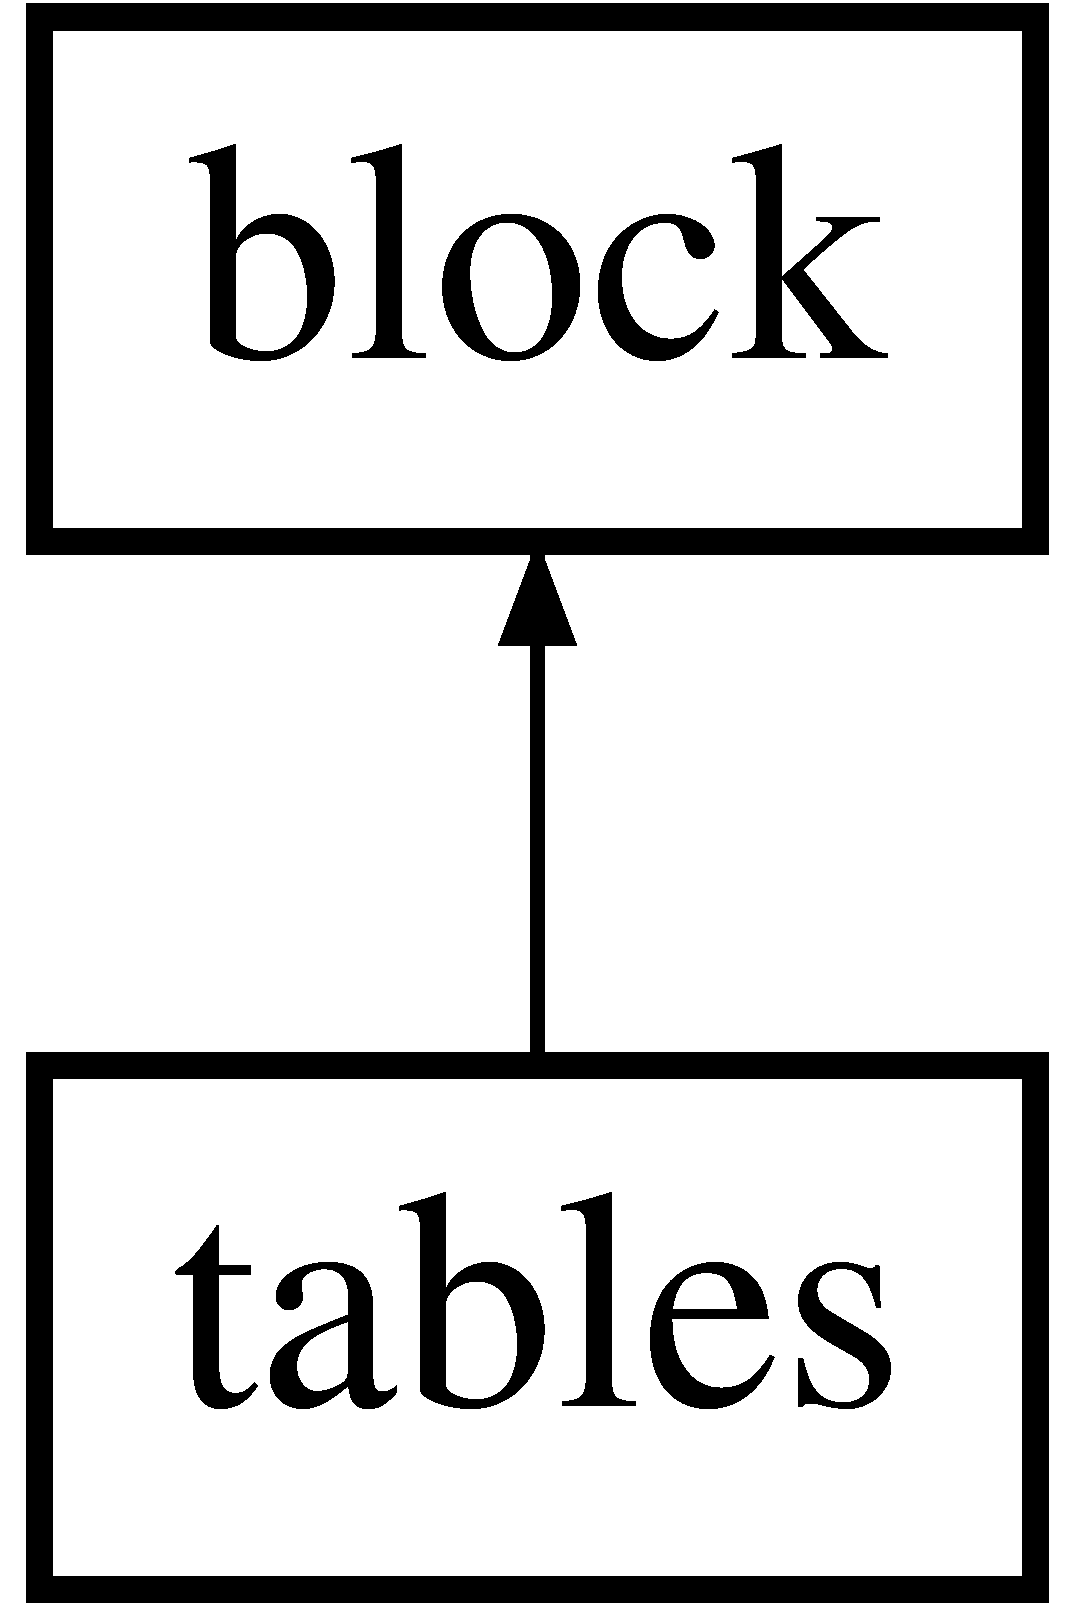
\includegraphics[height=2.000000cm]{classtables}
\end{center}
\end{figure}
\subsection*{\-Métodos públicos}
\begin{DoxyCompactItemize}
\item 
\hypertarget{classtables_abcd4e7cd574507fbd1fec1877a9cd72c}{{\bfseries show\-Table} (\$fn)}\label{classtables_abcd4e7cd574507fbd1fec1877a9cd72c}

\item 
\hypertarget{classtables_a7c9452dea1c737d4024d7560382f5f94}{{\bfseries units} (\$csv\-Line)}\label{classtables_a7c9452dea1c737d4024d7560382f5f94}

\item 
\hypertarget{classtables_a464fe5c5777973672ef774bdc1e95a43}{{\bfseries display} ()}\label{classtables_a464fe5c5777973672ef774bdc1e95a43}

\end{DoxyCompactItemize}


\subsection{\-Descripción detallada}


\-Definición en la línea 5 del archivo tables.\-php.



\-La documentación para esta clase fue generada a partir del siguiente fichero\-:\begin{DoxyCompactItemize}
\item 
tables.\-php\end{DoxyCompactItemize}

\hypertarget{classtitle}{}\section{Referencia de la Clase title}
\label{classtitle}\index{title@{title}}
Diagrama de herencias de title\begin{figure}[H]
\begin{center}
\leavevmode
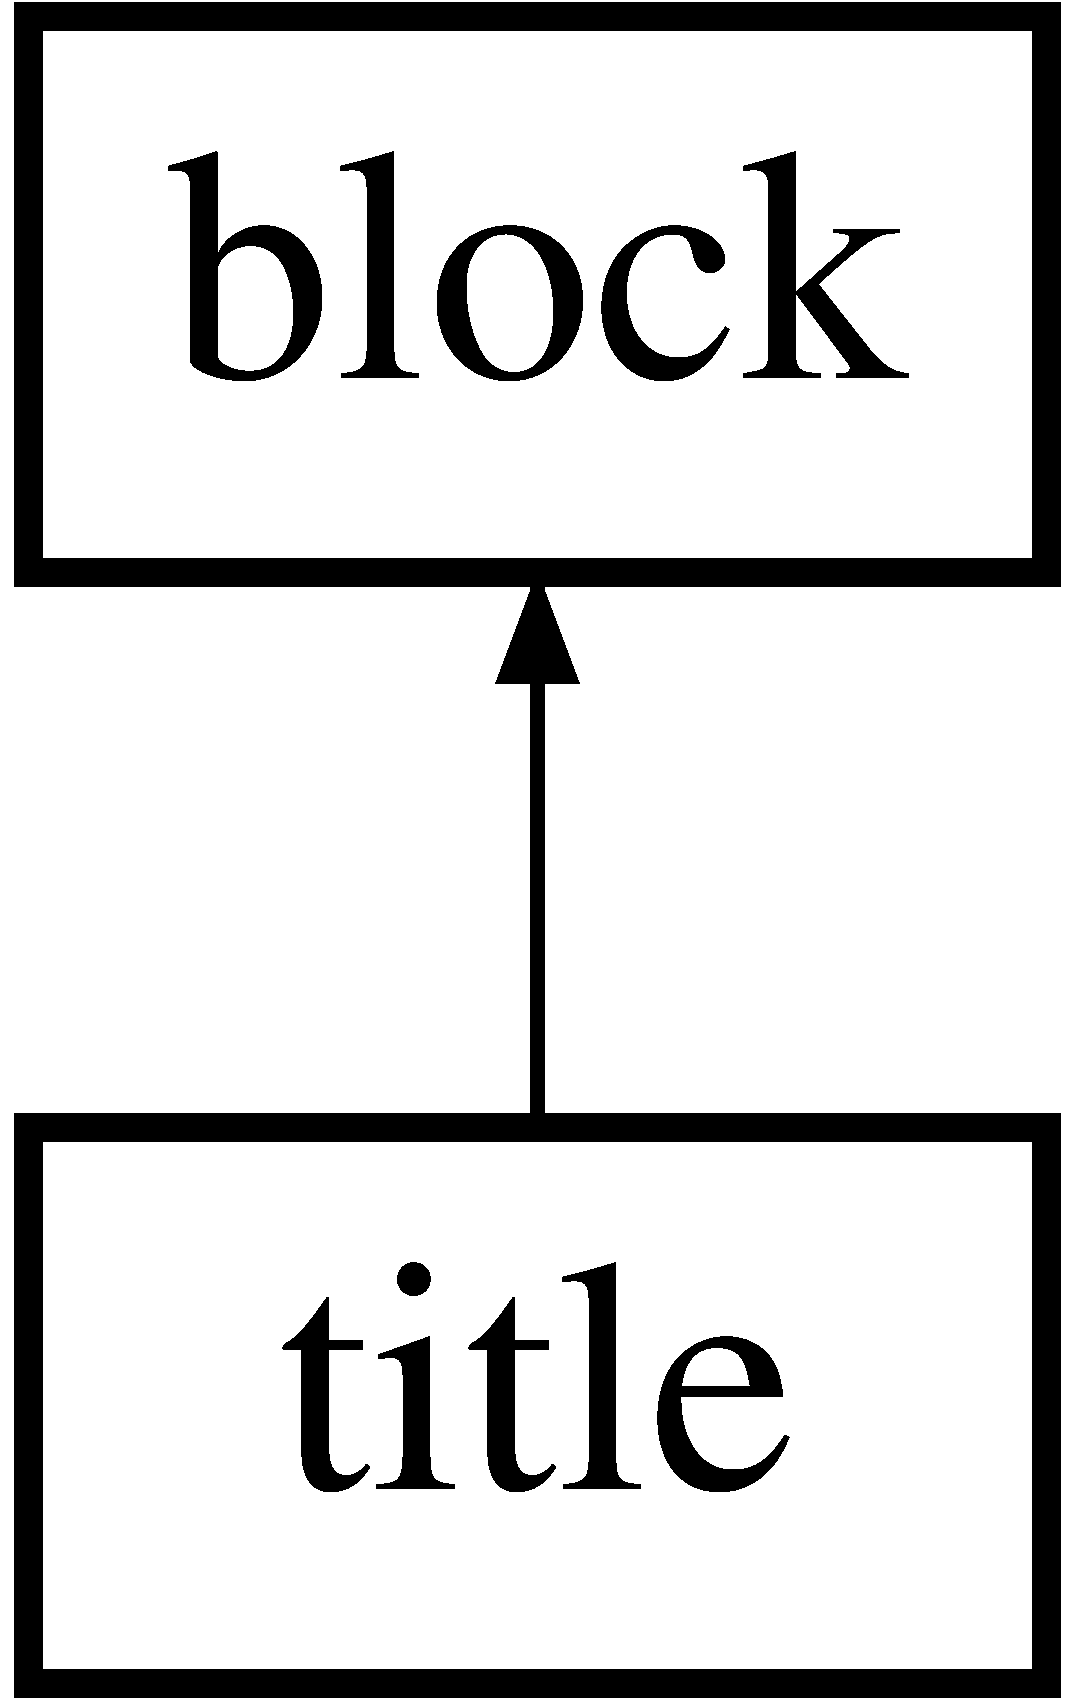
\includegraphics[height=2.000000cm]{classtitle}
\end{center}
\end{figure}
\subsection*{Métodos públicos}
\begin{DoxyCompactItemize}
\item 
\mbox{\Hypertarget{classtitle_a0b55e34d6485e20a3dfd4a6efd341ed8}\label{classtitle_a0b55e34d6485e20a3dfd4a6efd341ed8}} 
{\bfseries display} ()
\end{DoxyCompactItemize}
\subsection*{Otros miembros heredados}


\subsection{Descripción detallada}


Definición en la línea 4 del archivo title.\+php.



La documentación para esta clase fue generada a partir del siguiente fichero\+:\begin{DoxyCompactItemize}
\item 
/home/ogduartev/public\+\_\+html/unvl-\/\+Git\+Hub/\+U\+N\+Virtual\+Lab/title.\+php\end{DoxyCompactItemize}

\hypertarget{classtlistemysql}{\section{\-Referencia de la \-Clase tlistemysql}
\label{classtlistemysql}\index{tlistemysql@{tlistemysql}}
}
\subsection*{\-Métodos públicos}
\begin{DoxyCompactItemize}
\item 
\hypertarget{classtlistemysql_af1a889d94a44fc0762f01f1b493a5c32}{{\bfseries tlistemysql} (\$idd=\char`\"{}\char`\"{}, \$sf=\char`\"{}\char`\"{}, \$cc=\char`\"{}p1\char`\"{}, \$sqldata, \$condition=\char`\"{}\char`\"{})}\label{classtlistemysql_af1a889d94a44fc0762f01f1b493a5c32}

\item 
\hypertarget{classtlistemysql_a084df3acfe2c7828c1a3d999249022e0}{{\bfseries get\-Parameter} (\$sf)}\label{classtlistemysql_a084df3acfe2c7828c1a3d999249022e0}

\item 
\hypertarget{classtlistemysql_ab54c0101c71218747c16cefa3cff30e3}{{\bfseries read\-Mysql} (\$sqldata, \$id, \$level)}\label{classtlistemysql_ab54c0101c71218747c16cefa3cff30e3}

\item 
\hypertarget{classtlistemysql_a7007fb0857176648aeee18c73f059867}{{\bfseries display} ()}\label{classtlistemysql_a7007fb0857176648aeee18c73f059867}

\item 
\hypertarget{classtlistemysql_a1b00bffbd371386616d7ac066fb72d96}{{\bfseries add\-Elt} (\$xlt)}\label{classtlistemysql_a1b00bffbd371386616d7ac066fb72d96}

\item 
\hypertarget{classtlistemysql_accab70872d4dec1339c56cee4d9aebf4}{{\bfseries init\-Bar} ()}\label{classtlistemysql_accab70872d4dec1339c56cee4d9aebf4}

\item 
\hyperlink{classtlistemysql_a90b5cddbe5cda56f32fee824f6d345ba}{restore\-Node} ()
\item 
\hyperlink{classtlistemysql_a43c24fd4e27b46f3ac409d1a8a16623b}{save\-Node} ()
\end{DoxyCompactItemize}
\subsection*{\-Atributos públicos}
\begin{DoxyCompactItemize}
\item 
\hypertarget{classtlistemysql_a9ddf9ba93546488a287df97d2a8daadb}{{\bfseries \$\-\_\-id} = \char`\"{}\char`\"{}}\label{classtlistemysql_a9ddf9ba93546488a287df97d2a8daadb}

\item 
\hypertarget{classtlistemysql_ac5ee162a82a177093f9f141706ef63a2}{{\bfseries \$style}}\label{classtlistemysql_ac5ee162a82a177093f9f141706ef63a2}

\item 
\hypertarget{classtlistemysql_add32908fbfe4df9a2ffd1ede229220da}{{\bfseries \$image\-Path}}\label{classtlistemysql_add32908fbfe4df9a2ffd1ede229220da}

\item 
\hypertarget{classtlistemysql_a460438e1099c4aa1316fae91de2c7a26}{{\bfseries \$s\-File}}\label{classtlistemysql_a460438e1099c4aa1316fae91de2c7a26}

\item 
\hypertarget{classtlistemysql_ab0ec57d6c63919cacef728929e10d47c}{{\bfseries \$s\-Target}}\label{classtlistemysql_ab0ec57d6c63919cacef728929e10d47c}

\item 
\hypertarget{classtlistemysql_aeaf969d895757504965b1e9ec8349b47}{{\bfseries \$node}}\label{classtlistemysql_aeaf969d895757504965b1e9ec8349b47}

\item 
\hypertarget{classtlistemysql_a4a62b0b52e03ff4b956c064fc3a4f25d}{{\bfseries \$url}}\label{classtlistemysql_a4a62b0b52e03ff4b956c064fc3a4f25d}

\item 
\hypertarget{classtlistemysql_a8e145c2cd77d047f84108c3be5471c20}{{\bfseries \$param}}\label{classtlistemysql_a8e145c2cd77d047f84108c3be5471c20}

\item 
\hypertarget{classtlistemysql_a049bf18f5ffc940691d5e7d05daa8e7a}{{\bfseries \$ar\-Elt}}\label{classtlistemysql_a049bf18f5ffc940691d5e7d05daa8e7a}

\item 
\hypertarget{classtlistemysql_a6b42eb49fe2e32b077f09a93faf421dc}{{\bfseries \$nb\-Elt} = 0}\label{classtlistemysql_a6b42eb49fe2e32b077f09a93faf421dc}

\item 
\hypertarget{classtlistemysql_ae7d89c48e285747574bfe62f7476b20d}{{\bfseries \$lnode} = 0}\label{classtlistemysql_ae7d89c48e285747574bfe62f7476b20d}

\item 
\hypertarget{classtlistemysql_a9dbf35cbe30b6f9708e11ee904071792}{{\bfseries \$i\-Open} = 0}\label{classtlistemysql_a9dbf35cbe30b6f9708e11ee904071792}

\item 
\hypertarget{classtlistemysql_a5f13fa5afd2eec1af265cbfa1fc78382}{{\bfseries \$condition} = \char`\"{}\char`\"{}}\label{classtlistemysql_a5f13fa5afd2eec1af265cbfa1fc78382}

\end{DoxyCompactItemize}


\subsection{\-Descripción detallada}


\-Definición en la línea 18 del archivo tlistemysql.\-php.



\subsection{\-Documentación de las funciones miembro}
\hypertarget{classtlistemysql_a90b5cddbe5cda56f32fee824f6d345ba}{\index{tlistemysql@{tlistemysql}!restore\-Node@{restore\-Node}}
\index{restore\-Node@{restore\-Node}!tlistemysql@{tlistemysql}}
\subsubsection[{restore\-Node}]{\setlength{\rightskip}{0pt plus 5cm}{\bf tlistemysql\-::restore\-Node} (
\begin{DoxyParamCaption}
{}
\end{DoxyParamCaption}
)}}\label{classtlistemysql_a90b5cddbe5cda56f32fee824f6d345ba}
restore\-Node \-: restore nodes states 

\-Definición en la línea 273 del archivo tlistemysql.\-php.


\begin{DoxyCode}
  {
  //  global $lnode, $node, $arElt ;
  
    if (is_null($this->node) || trim($this->node) === "") return ;
          
    $this->lnode = doubleval($this->node) ;
    $iNo = 0 ;
  
    for ($i=0; $i<count($this->arElt); $i=$i+1)
    {
      $elt = $this->arElt[$i] ;
      if ( $elt->iS > -1) 
      {
        $l = $this->lnode & (1 << $iNo) ;                
        if ($l) 
          $elt->open() ;
        else
            $elt->close() ;
        $iNo++ ;
      }
    }
  }
\end{DoxyCode}
\hypertarget{classtlistemysql_a43c24fd4e27b46f3ac409d1a8a16623b}{\index{tlistemysql@{tlistemysql}!save\-Node@{save\-Node}}
\index{save\-Node@{save\-Node}!tlistemysql@{tlistemysql}}
\subsubsection[{save\-Node}]{\setlength{\rightskip}{0pt plus 5cm}{\bf tlistemysql\-::save\-Node} (
\begin{DoxyParamCaption}
{}
\end{DoxyParamCaption}
)}}\label{classtlistemysql_a43c24fd4e27b46f3ac409d1a8a16623b}
save\-Node \-: build lnode value 

\-Definición en la línea 300 del archivo tlistemysql.\-php.


\begin{DoxyCode}
  {
  //  global $lnode, $arElt ;
  
    /* for each elements */
    $iNo = 0 ;
  
    for ($i=0; $i<count($this->arElt); $i=$i+1)
    {
      $elt = $this->arElt[$i] ;
      if ( $elt->iS > -1) 
      {
        if ( $elt->iS > 0) 
        {
          $this->lnode = $this->lnode | (1 << $iNo) ;                
        }
        $iNo++ ;
      }
    }
  }
\end{DoxyCode}


\-La documentación para esta clase fue generada a partir del siguiente fichero\-:\begin{DoxyCompactItemize}
\item 
phptliste/tlistemysql.\-php\end{DoxyCompactItemize}

\hypertarget{classXMLThing}{\section{\-Referencia de la \-Clase \-X\-M\-L\-Thing}
\label{classXMLThing}\index{\-X\-M\-L\-Thing@{\-X\-M\-L\-Thing}}
}
\subsection*{\-Métodos públicos}
\begin{DoxyCompactItemize}
\item 
\hyperlink{classXMLThing_a1c153caf15cb3b1a2159d5e879a3f6ca}{\-X\-M\-L\-Thing} (\$xml=\-N\-U\-L\-L)
\item 
\hyperlink{classXMLThing_a8d408058141c8a030b433b2deb822baf}{parse} (\$xml=\-N\-U\-L\-L)
\item 
\hyperlink{classXMLThing_ae18a74c5d5979c699b42b1f9a8fedbba}{parse\-\_\-recurse} ()
\item 
\hyperlink{classXMLThing_aa5d425088bd74ca4f3f9c1a9bc9ac453}{parse\-\_\-init} ()
\end{DoxyCompactItemize}
\subsection*{\-Atributos públicos}
\begin{DoxyCompactItemize}
\item 
\hypertarget{classXMLThing_a07538f3f144881632ffd11d3699e5562}{{\bfseries \$raw\-X\-M\-L}}\label{classXMLThing_a07538f3f144881632ffd11d3699e5562}

\item 
\hypertarget{classXMLThing_a0c4f39e54503d71299dc274d787dd0f3}{{\bfseries \$value\-Array} = array()}\label{classXMLThing_a0c4f39e54503d71299dc274d787dd0f3}

\item 
\hypertarget{classXMLThing_a49615464bf3ef0a0ef606179ff55afc1}{{\bfseries \$key\-Array} = array()}\label{classXMLThing_a49615464bf3ef0a0ef606179ff55afc1}

\item 
\hypertarget{classXMLThing_a0f4ddacd5ff9a4dabcbddc39aa47f9c5}{{\bfseries \$parsed} = array()}\label{classXMLThing_a0f4ddacd5ff9a4dabcbddc39aa47f9c5}

\item 
\hypertarget{classXMLThing_a9165f7eec1b7840c6076b294ef497f68}{{\bfseries \$index} = 0}\label{classXMLThing_a9165f7eec1b7840c6076b294ef497f68}

\item 
\hypertarget{classXMLThing_a658a4bd3bff6ade05283ad48aec5379b}{{\bfseries \$attrib\-Key} = 'attributes'}\label{classXMLThing_a658a4bd3bff6ade05283ad48aec5379b}

\item 
\hypertarget{classXMLThing_a9948e8517f8b349298a20d9286a3b2b7}{{\bfseries \$value\-Key} = 'value'}\label{classXMLThing_a9948e8517f8b349298a20d9286a3b2b7}

\item 
\hypertarget{classXMLThing_a445699d05b90f941d5b09ad3331da61a}{{\bfseries \$cdata\-Key} = 'cdata'}\label{classXMLThing_a445699d05b90f941d5b09ad3331da61a}

\item 
\hypertarget{classXMLThing_a4d29070c404490ab9ef64c44485fb330}{{\bfseries \$is\-Error} = false}\label{classXMLThing_a4d29070c404490ab9ef64c44485fb330}

\item 
\hypertarget{classXMLThing_afd5fee61b2486f3c5f03b0da62f69b62}{{\bfseries \$error} = ''}\label{classXMLThing_afd5fee61b2486f3c5f03b0da62f69b62}

\end{DoxyCompactItemize}


\subsection{\-Descripción detallada}
\begin{DoxyAuthor}{\-Autor}
wickedfather at hotmail.\-com
\end{DoxyAuthor}
\-P\-H\-P4 and \-P\-H\-P5 compatible

14th \-Apr cdata\-Key index for open tags fixed \-Class to parse xml into an array the way \-I like it.

\begin{DoxyAuthor}{\-Autor}
wickedfather at hotmail.\-com 
\end{DoxyAuthor}
\begin{DoxyVersion}{\-Versión}
0.\-0.\-2 
\end{DoxyVersion}


\-Definición en la línea 17 del archivo xmlthing.\-class.\-php.



\subsection{\-Documentación de las funciones miembro}
\hypertarget{classXMLThing_a8d408058141c8a030b433b2deb822baf}{\index{\-X\-M\-L\-Thing@{\-X\-M\-L\-Thing}!parse@{parse}}
\index{parse@{parse}!XMLThing@{\-X\-M\-L\-Thing}}
\subsubsection[{parse}]{\setlength{\rightskip}{0pt plus 5cm}{\bf \-X\-M\-L\-Thing\-::parse} (
\begin{DoxyParamCaption}
\item[{\$}]{xml = {\ttfamily \-N\-U\-L\-L}}
\end{DoxyParamCaption}
)}}\label{classXMLThing_a8d408058141c8a030b433b2deb822baf}
\-Turns xml into a lovely array 
\begin{DoxyParams}{\-Parámetros}
{\em string} & option xml to parse. \-That supplied to constructor used otherwise. \\
\hline
\end{DoxyParams}
\begin{DoxyReturn}{\-Devuelve}
array parsed data 
\end{DoxyReturn}


\-Definición en la línea 61 del archivo xmlthing.\-class.\-php.


\begin{DoxyCode}
        {
                if (!is_null($xml))
                {
                        $this->rawXML = $xml;
                }

                $this->isError = false;
                        // setup
                if (!$this->parse_init())
                {
                        return false;
                }

                $this->index = 0;
                $this->parsed = $this->parse_recurse();
                $this->status = 'parsing complete';

                return $this->parsed;
        }
\end{DoxyCode}
\hypertarget{classXMLThing_aa5d425088bd74ca4f3f9c1a9bc9ac453}{\index{\-X\-M\-L\-Thing@{\-X\-M\-L\-Thing}!parse\-\_\-init@{parse\-\_\-init}}
\index{parse\-\_\-init@{parse\-\_\-init}!XMLThing@{\-X\-M\-L\-Thing}}
\subsubsection[{parse\-\_\-init}]{\setlength{\rightskip}{0pt plus 5cm}{\bf \-X\-M\-L\-Thing\-::parse\-\_\-init} (
\begin{DoxyParamCaption}
{}
\end{DoxyParamCaption}
)}}\label{classXMLThing_aa5d425088bd74ca4f3f9c1a9bc9ac453}
\-Turns the xml into the array pairs with xml\-\_\-parse\-\_\-into\-\_\-struct \begin{DoxyReturn}{\-Devuelve}
bool 
\end{DoxyReturn}


\-Definición en la línea 186 del archivo xmlthing.\-class.\-php.


\begin{DoxyCode}
        {
        $this->parser = xml_parser_create();

        $parser = $this->parser;
        xml_parser_set_option($parser, XML_OPTION_CASE_FOLDING, 0);     // Dont
       mess with my cAsE sEtTings
        xml_parser_set_option($parser, XML_OPTION_SKIP_WHITE, 1);               
      // Dont bother with empty info
        if (!$res = (bool)xml_parse_into_struct($parser, $this->rawXML, $this->
      valueArray, $this->keyArray))
                {
                        $this->isError = true;
            $this->error = 'error: '.xml_error_string(xml_get_error_code(
      $parser)).' at line '.xml_get_current_line_number($parser);
        }
        xml_parser_free($parser);

                return $res;
        }
\end{DoxyCode}
\hypertarget{classXMLThing_ae18a74c5d5979c699b42b1f9a8fedbba}{\index{\-X\-M\-L\-Thing@{\-X\-M\-L\-Thing}!parse\-\_\-recurse@{parse\-\_\-recurse}}
\index{parse\-\_\-recurse@{parse\-\_\-recurse}!XMLThing@{\-X\-M\-L\-Thing}}
\subsubsection[{parse\-\_\-recurse}]{\setlength{\rightskip}{0pt plus 5cm}{\bf \-X\-M\-L\-Thing\-::parse\-\_\-recurse} (
\begin{DoxyParamCaption}
{}
\end{DoxyParamCaption}
)}}\label{classXMLThing_ae18a74c5d5979c699b42b1f9a8fedbba}
\-Turns the struct array into a nested one \begin{DoxyReturn}{\-Devuelve}
array 
\end{DoxyReturn}


\-Definición en la línea 88 del archivo xmlthing.\-class.\-php.


\begin{DoxyCode}
        {               // data found at this level
                $found = array();
                        // count of the number of times a tag has been found at
       this level
                $tagCount = array();

                        // loop through the tags - I use a lazy referencing
       thing for where data should go

                while (isset($this->valueArray[$this->index]))
                {
                        $tag = $this->valueArray[$this->index];
                        $this->index++;

                                // if it's a close then return straight away

                        if ($tag['type'] == 'close')
                        {
                                return $found;
                        }
                                // if it's cdata translate it as a complete tag
       named $this->cdataKey
                        if ($tag['type'] == 'cdata')
                        {
                                $tag['tag'] = $this->cdataKey;
                                $tag['type'] = 'complete';
                        }

                        $tagName = $tag['tag'];

                                // this bit below creates a reference to where
       the data should be going, 
                                // it saves on some conditions in the switch,
       but it probably annoyingly obfuscating
                                // has this tag already appeared at this level
       ?  If so we need mods

                        if (isset($tagCount[$tagName]))
                        {               // transform to an array IF only one of
       the tags been before
                                if ($tagCount[$tagName] == 1)
                                {
                                        $found[$tagName] = array($found[
      $tagName]);
                                }
                                        //$found[$tagName][$tagCount[$tagName]]
       = '';   // doesn't need to happen, the reference below is enough
                                $tagRef =& $found[$tagName][$tagCount[$tagName]
      ];
                                $tagCount[$tagName]++;
                        }
                        else    // just use the variable
                        {
                                $tagCount[$tagName] = 1;
                                $tagRef =& $found[$tagName];
                        }

                                // now do the work

                        switch ($tag['type'])
                        {
                                case 'open':
                                        $tagRef = $this->parse_recurse();

                                        if (isset($tag['attributes']))
                                        {
                                                $tagRef[$this->attribKey] = 
      $tag['attributes'];
                                        }
                                                // open CAN have a value - it
       makes sense to include it as cdata
                                        if (isset($tag['value']))
                                        {
                                                if (isset($tagRef[$this->
      cdataKey]))    // push it to the start of the cdata array if it's present
                                                {
                                                        $tagRef[$this->cdataKey
      ] = (array)$tagRef[$this->cdataKey];     // <-- needed for php5 compatibility];
                                                        array_unshift($tagRef[
      $this->cdataKey], $tag['value']);
                                                }
                                                else
                                                {
                                                        $tagRef[$this->cdataKey
      ] = $tag['value'];
                                                }
                                        }
                                        break;

                                case 'complete':
                                        if (isset($tag['attributes']))
                                        {
                                                $tagRef[$this->attribKey] = 
      $tag['attributes'];
                                                $tagRef =& $tagRef[$this->
      valueKey];
                                        }

                                        if (isset($tag['value']))
                                        {
                                                $tagRef = $tag['value'];
                                        }
                                        break;
                        }                       
                }

                return $found;
        }
\end{DoxyCode}
\hypertarget{classXMLThing_a1c153caf15cb3b1a2159d5e879a3f6ca}{\index{\-X\-M\-L\-Thing@{\-X\-M\-L\-Thing}!\-X\-M\-L\-Thing@{\-X\-M\-L\-Thing}}
\index{\-X\-M\-L\-Thing@{\-X\-M\-L\-Thing}!XMLThing@{\-X\-M\-L\-Thing}}
\subsubsection[{\-X\-M\-L\-Thing}]{\setlength{\rightskip}{0pt plus 5cm}{\bf \-X\-M\-L\-Thing\-::\-X\-M\-L\-Thing} (
\begin{DoxyParamCaption}
\item[{\$}]{xml = {\ttfamily \-N\-U\-L\-L}}
\end{DoxyParamCaption}
)}}\label{classXMLThing_a1c153caf15cb3b1a2159d5e879a3f6ca}
\-Constructor 
\begin{DoxyParams}{\-Parámetros}
{\em string} & xml data to parse -\/ optional \\
\hline
\end{DoxyParams}


\-Definición en la línea 49 del archivo xmlthing.\-class.\-php.


\begin{DoxyCode}
        {
        $this->rawXML = $xml;
    }
\end{DoxyCode}


\-La documentación para esta clase fue generada a partir del siguiente fichero\-:\begin{DoxyCompactItemize}
\item 
xmlthing.\-class.\-php\end{DoxyCompactItemize}

%--- End generated contents ---

% Index
\backmatter
\newpage
\phantomsection
\clearemptydoublepage
\addcontentsline{toc}{chapter}{Índice}
\printindex

\end{document}
